\documentclass[11pt,oneside,a4paper]{article}
\usepackage{graphicx}
\usepackage{booktabs}
\usepackage{caption}
\usepackage{subcaption}
\usepackage{amsmath}
\usepackage{amsfonts}
\usepackage{amssymb}
\usepackage{lscape}
\usepackage{psfrag}
\usepackage[usenames]{color}
\usepackage{bbm}
\usepackage[update]{epstopdf}
\usepackage[bookmarks,pdfstartview=FitH,a4paper,pdfborder={0 0 0}]{hyperref}
\usepackage{verbatim}
\usepackage{listings}
\usepackage{textcomp}
\usepackage{fancyhdr}
\usepackage{multirow}
\usepackage{multicol}
\usepackage{tikz}
\usepackage{lipsum}
\usepackage{xcolor}
\usepackage{wrapfig}
\usepackage[margin=0.5in]{geometry}
\usepackage{pdfpages}
\usepackage[utf8]{inputenc}
\usepackage[compact]{titlesec}
\usepackage{paralist}
\usepackage{makecell}
\newcommand{\hint}[1]{{\color{blue} \em #1}}
\usepackage{listings}
\usepackage{ccicons}

\usepackage{color}
\definecolor{gray}{rgb}{0.4,0.4,0.4}
\definecolor{darkblue}{rgb}{0.0,0.0,0.6}
\definecolor{cyan}{rgb}{0.0,0.6,0.6}

\lstset{
	basicstyle=\ttfamily,
	columns=fullflexible,
	showstringspaces=false,
	commentstyle=\color{gray}\upshape
}

\lstdefinelanguage{XML}
{
	morestring=[b]",
	morestring=[s]{>}{<},
	morecomment=[s]{<?}{?>},
	stringstyle=\color{black},
	identifierstyle=\color{darkblue},
	keywordstyle=\color{cyan},
	morekeywords={xmlns,version,type}% list your attributes here
}

\makeatletter %% <- make @ usable in command names
\newcommand*\Neg[2][0mu]{\Neginternal{#1}{\negslash}{#2}}
\newcommand*\sNeg[2][0mu]{\Neginternal{#1}{\snegslash}{#2}}
\newcommand*\ssNeg[2][0mu]{\Neginternal{#1}{\ssnegslash}{#2}}
\newcommand*\sssNeg[2][0mu]{\Neginternal{#1}{\sssnegslash}{#2}}
\newcommand*\Neginternal[3]{\mathpalette\Neg@{{#1}{#2}{#3}}}
\newcommand*\Neg@[2]{\Neg@@{#1}#2}
\newcommand*\Neg@@[4]{%
	\mathrel{\ooalign{%
			$\m@th#1#4$\cr
			\hidewidth$\m@th#3{#1}\mkern\muexpr#2*2$\hidewidth\cr
	}}%
}

\newcommand*\negslash[1]{\m@th#1\not\mathrel{\phantom{=}}}
\newcommand*\snegslash[1]{\rotatebox[origin=c]{60}{$\m@th#1-$}}
\newcommand*\ssnegslash[1]{\rotatebox[origin=c]{60}{$\m@th#1{\dabar@}\mkern-7mu{\dabar@}$}}
\newcommand*\sssnegslash[1]{\rotatebox[origin=c]{60}{$\m@th#1\dabar@$}}
\makeatother  %% <- revert @

\def\cleardoublepage{\clearpage\if@twoside \ifodd\c@page\else%
\hbox{}%
\thispagestyle{empty}%
\clearpage%
\if@twocolumn\hbox{}\clearpage\fi\fi\fi}
\makeatother

\sloppy
% \widowpenalty=10000
% \clubpenalty=10000

\title{Big Data for Engineers}
\author{Yannick Merkli, \texttt{ymerkli@ethz.ch}}
\date{ETH Zurich, FS 2020}

\begin{document}

\begin{titlepage}
\maketitle
\vspace{3cm}
\thispagestyle{empty}


\begin{abstract}
	\noindent This document is a "lecture summary" style script that closely follows the slides of the \textit{Big Data for Engineers} lecture  at ETH Zurich. The contribution to this is editing and refactoring as well as providing additional material for better understanding. This summary was created during the spring semester 2020. Due to updates to the syllabus content, some material may no longer be relevant for future versions of the lecture.\\
	Most graphics are copy \& pasted from the slides. If you don't want yours here, please contact me and I will remove them. Otherwise, this work is published as CC BY-NC-SA.
	
	\begin{center}
		\ccbyncsa
	\end{center}
	
	\noindent I do not guarantee correctness or completeness, nor is this document endorsed by the lecturers. Feel free to point out any erratas. For the full \LaTeX \ source code, consider \texttt{\href{https://github.com/ymerkli/eth-summaries}{github.com/ymerkli/eth-summaries}}.
\end{abstract}

\end{titlepage}

\maketitle
\thispagestyle{empty}
\raggedbottom
\clearpage

\pagenumbering{roman}

\clearpage
\setcounter{tocdepth}{2}
\tableofcontents
\clearpage
\pagenumbering{arabic}
\setlength\parindent{0pt}

\section{Introduction}

\subsection{History}

Databases have always existed in some way as a way to preserve information. It started with speaking and singing, went on with stone engraving and printing. Even before computers, tables were the primary format to represent data. Things changed drastically with the introduction of computers. Database management systems (DBMS) started with file systems (1960s), then we entered the relational era (1970s) and finally progressed into the NoSQL era (2000s) with the upcoming of big data.

\subsection{Big Data}

Big Data is a buzzword that goes across many disciplines (distributed systems, high-performance computing, data management, algorithms, statistics, machine learning, etc.) and that involves a lot of proprietary technology (AWS, Google Cloud, Microsoft Azure, etc.) which is simply a result of the need of companies to have efficient data systems.

The big in big data: \textbf{three Vs}

\vspace{-\topsep}
\begin{itemize}
	\setlength{\itemsep}{0pt}
	\setlength{\parskip}{0pt}
	\item Volume: Nowadays we have lots of sources of data (web, sensors, proprietary, scientific). Storage has become so cheap that we often just store data because we can. Further, data carries value; data is worth more than the sum of its parts (data totality: one must have complete data).
	\item Variety: We have different \textbf{data shapes}: tables, trees, graphs, cubes, text.
	\item Velocity: Data is generated automatically, Data is a realtime byproduct of human activity
\end{itemize}

\textbf{Prefixes (International System of Units)}

\begin{tabular}{|c|r|c|r|}
	\hline 
	kilo (k) & 1,000 (3 zeros) & kibi (ki) & 1,024 ($2^{10}$) \\ 
	\hline 
	Mega (M) & 1,000,000 (6 zeros) & Mebi (Mi) & 1,048,576 ($2^{20}$) \\ 
	\hline 
	Giga (G) & 1,000,000,000 (9 zeros) & Gibi (Gi) & 1,073,741,824 ($2^{30}$) \\ 
	\hline 
	Tera (T) & 1,000,000,000,000 (12 zeros) & Tebi (Ti) & 1,099,511,627,776 ($2^{40}$) \\ 
	\hline 
	Peta (P) & 1,000,000,000,000,000 (15 zeros) & Pebi (Pi) & 1,125,899,906,842,624 ($2^{50}$) \\ 
	\hline 
	Exa (E) & 1,000,000,000,000,000,000 (18 zeros) & Exbi (Ei) & 1,152,921,504,606,846,976 ($2^{60}$) \\ 
	\hline 
	Zetta (Z) & 1,000,000,000,000,000,000,000 (21 zeros) & Zebi (Zi) & 1,180,591,620,717,411,303,424 ($2^{70}$) \\ 
	\hline 
	Yotta (Y) & 1,000,000,000,000,000,000,000,000 (24 zeros) & Yobi (Yi) & 1,208,925,819,614,629,174,706,176 ($2^{80}$) \\ 
	\hline
\end{tabular}\newline

There are three paramount factors to big data:

\vspace{-\topsep}
\begin{itemize}
	\setlength{\itemsep}{0pt}
	\setlength{\parskip}{0pt}
	\item Capacity: "How much data can we store?"
	\item Throughput: "How fast can we transmit data?"
	\item Latency: "When do I start receiving data?"
\end{itemize}
\vspace{-\topsep}

Capacity has improved incredibly much over the past 60 years (1956: huge HDD had 5MB storage, 2020: there are palm sized 20TB HDDs). Capacity has increased by a factor $200 * 10^9$ (per unit of volume). However, throughput and latency have only improved by a factor $10'000$ and $8$ respectively. This discrepancy creates problems: the throughput no longer scales to the amount of data and the latency no longer scales to the throughput. Solution:

\vspace{-\topsep}
\begin{itemize}
	\setlength{\itemsep}{0pt}
	\setlength{\parskip}{0pt}
	\item Capacity-throughput discrepancy: parallelization
	\item Throughput-latency discrepancy: batch processing
\end{itemize}
\vspace{-\topsep}

\textbf{What is big data?}

Big Data is a portfolio of technologies that were designed to store, manage and analyze data that is too large to fit on a single machine while accommodating for the issue of growing discrepancy between
capacity, throughput and latency.

\section{Lessons learnt from the past}

\textbf{Data Independence:}\\
An underlying principle that has been valid for a long time is the principle of \textbf{data independence} (developed by Edgar Codd): Data Independence is defined as a property of DBMS that helps you to change the Database schema at one level of a database system without requiring to change the schema at the next higher level. Data independence helps you to keep data separated from all programs that make use of it.\\
This means we could e.g. change the physical storage (e.g. iPad instead of HDD) \textit{without} changing the logical data model.\\

\textbf{Data shapes:} Text, trees, tables, graphs, cubes.

\textbf{Overall architecture}\\
The overall architecture of a DBMS consists of:

\vspace{-\topsep}
\begin{itemize}
	\setlength{\itemsep}{0pt}
	\setlength{\parskip}{0pt}
	\item Language (e.g. SQL)
	\item Model (e.g. Tables (old), graphs, trees, cubes (new)
	\item Compute (e.g. single CPU (old), hadoop cluster (new))
	\item Storage (e.g. HDD (old), distributed storage (new))
\end{itemize}
\vspace{-\topsep}

A data model essentially describes \textit{what data looks like} and \textit{what you can do with the data}.

\subsection{Basic concepts}

\begin{itemize}
	\setlength{\itemsep}{0pt}
	\setlength{\parskip}{0pt}
	\item Table (Collection): A set of rows (= business object, item, entity, document, record) and each row has attributes (= columns)
	\item Attribute (column, field, property): A certain attribute of a row
	\item Primary key (row ID, name): a unique identifier of a row
\end{itemize}
\vspace{-\topsep}

\subsection{Relational Algebra}

We can look at tables as relations or as partial functions, mapping property to value\\
($f \in \mathbb{S} \ssNeg \rightarrow \mathbb{V}$), e.g. $city \mapsto Zurich$.

\subsubsection{Relations (the math, for database scientists)}

A relation R is made of:
\vspace{-\topsep}
\begin{itemize}
	\setlength{\itemsep}{0pt}
	\setlength{\parskip}{0pt}
	\item A set of attributes: $Attributes_R \subseteq \mathbb{S}$
	\item An extension (set of tuples): $$Extension_R \subseteq \mathbb{S} \ssNeg \rightarrow \mathbb{V} \quad s.t. \quad \forall t \in Extension_R, support(t) = Attributes_R$$
\end{itemize}
\vspace{-\topsep}

\textbf{Tabular integrity:} Holds if all rows have the same attributes and have a value for the attributes.\\
\textbf{Atomic integrity (1st normal form):} No tables in tables.\\
\textbf{Domain integrity:} All attribute values are of the specified type (e.g. an attribute \textit{Name} of type string can't be an integer).\\

In SQL, tabular integrity, atomic integrity and domain integrity all hold. In NoSQL however, none of these three properties hold.

\subsection{The relational model of data}

\begin{compactitem}
	\item Data Models: A data model is a notation for describing the structure of the data in a database, along with the constraints on that data. The data	model also normally provides a notation for describing operations on that data: queries and data modifications.
	\item Relational Model: Relations are tables representing information. Columns are headed by attributes; each attribute has an associated domain, or	data type. Rows are called tuples, and a tuple has one component for each attribute of the relation.
	\item Schemas: A relation name, together with the attributes of that relation and their types, form the relation schema. A collection of relation schemas forms a database schema. Particular data for a relation or collection of relations is called an instance of that relation schema or database schema.
	\item Keys: An important type of constraint on relations is the assertion that an attribute or set of attributes forms a key for the relation. No two tuples of a relation can agree on all attributes of the key, although they can agree on some of the key attributes.
	\item Semistructured Data Model: In this model, data is organized in a tree or graph structure. XML is an important example of a semistructured data model.
	\item SQL: The language SQL is the principal query language for relational database systems. The current standard is called SQL-99. Commercial systems generally vary from this standard but adhere to much of it.
	\item Data Definition: SQL has statements to declare elements of a database schema. The CREATE TABLE statement allows us to declare the schema for stored relations (called tables), specifying the attributes, their types, default values, and keys.
	\item Altering Schemas: We can change parts of the database schema with an ALTER statement. These changes include adding and removing attributes from relation schemas and changing the default value associated with an attribute. We may also use a DROP statement to completely eliminate relations or other schema elements.
	\item Relational Algebra: This algebra underlies most query languages for the relational model. Its principal operators are union, intersection, difference, selection, projection, Cartesian product, natural join, theta-join, and renaming.
	\item Selection and Projection: The selection operator produces a result consisting of all tuples of the argument relation that satisfy the selection condition. Projection removes undesired columns from the argument relation to produce the result.
	\item Joins: We join two relations by comparing tuples, one from each relation.	In a natural join, we splice together those pairs of tuples that agree on all attributes common to the two relations. In a theta-join, pairs of tuples are concatenated if they meet a selection condition associated with the theta-join.
	\item Grouping: Aggregate multiple rows by some attribute.
	\item Sorting: Sort rows by some attribute.
	\item Constraints in Relational Algebra: Many common kinds of constraints can be expressed as the containment of one relational algebra expression in another, or as the equality of a relational algebra expression to the empty set.
\end{compactitem}

\subsection{Relational queries}

The following table shows the operators used in Relational Algebra.

\vspace{-\topsep}
\begin{figure}[hb]
	\centering
	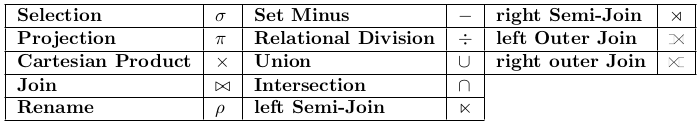
\includegraphics[width=0.7\linewidth]{figures/relational_algebra_operators}
	\label{fig:relationalalgebraoperators}
\end{figure}
\vspace{-\topsep}

\textbf{Projection:} The projection operator is used to produce from a relation R a new relation that has only some of R’s columns. The value of expression $\prod_{A_1,...,A_n}(R)$ is a relation that only
consists of columns for the attributes $A_1,...,A_n$.

\textbf{Selection:} The selection operator applied to R produces a new relation with a subset of R’s tuples, namely those who meet some condition C. This operation is denoted by $\sigma_C(R)$.

\textbf{Cartesian product:} The Cartesian product of relations R, S, denoted $R \times S$, simply concatenates every possible combination of tuples $r \in R, s \in S$. If R, S have attributes in common: rename them. In practice rarely used without join operators.

\textbf{Natural Join:} The natural join of relations L, R, denoted $L \bowtie R$, pairs only those tuples from L and R that agree in whatever attributes they share commonly. Natural Join is associative!
Other variants:

\vspace{-\topsep}
\begin{itemize}
	\setlength{\itemsep}{0pt}
	\setlength{\parskip}{0pt}
	\item Left outer join: natural join \& unmatched tuples from L
	\item Right outer join: natural join \& unmatched tuples from R
	\item Full outer join: natural join \& unmatched tuples from both L and R
	\item Left semi join: tuples from L that match with some tuple in R
	\item Right semi join: tuples from R that match with some tuple in L
\end{itemize}
\vspace{-\topsep}

\textbf{Theta-Join:} A theta join $\bowtie_\theta$ allows to join tuples from two relations R, S based on an arbitrary condition $\theta$ rather than solely based on attribute agreement. We get this new relation by:

\vspace{-\topsep}
\begin{enumerate}
	\setlength{\itemsep}{0pt}
	\setlength{\parskip}{0pt}
	\item Take the Cartesian product $R \times S$
	\item select those tuples satisfying condition $\theta$
\end{enumerate}
\vspace{-\topsep}

\textbf{Union, Intersection, Set Minus:} requires: both relations have the same schema $\rightarrow$ then consider set of tuples, do corresponding set operations. Note that $R \cap S = R - (R - S)$

\textbf{Rename:} 

\vspace{-\topsep}
\begin{itemize}
	\setlength{\itemsep}{0pt}
	\setlength{\parskip}{0pt}
	\item to change the name of the relation R to S, we write $\rho_S(R)$. 
	\item to rename attributes of R, we use the operator $\rho_{(A_1,..,A_n)}(R)$ where the attributes in the result relation S are called $A_1,...,A_n$, respectively.
\end{itemize}
\vspace{-\topsep}

\newpage

\subsection{Terminology}

Data: Data Manipulation Language (DML) (Query, insert, remove rows)
Schema: Data Definition Language (DDL) (Create or table/schema, drop it)
\vspace{-\topsep}
\begin{figure}[hb!]
	\centering
	\begin{subfigure}[t]{.5\textwidth}
		\centering
		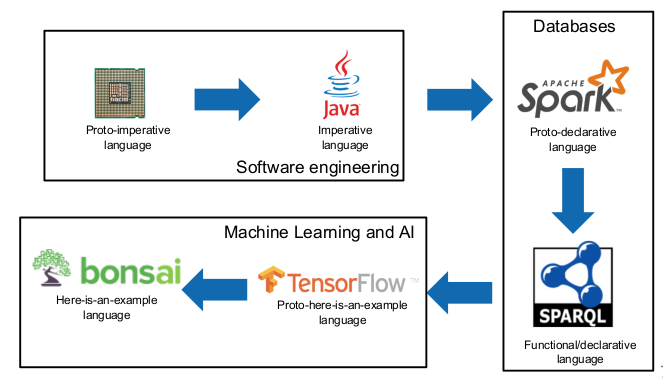
\includegraphics[width=0.8\linewidth]{figures/language_landscape}
		\caption{Language landscape}
		\label{fig:languagelandscape}
	\end{subfigure}%
	\begin{subfigure}[t]{.5\textwidth}
		\centering
		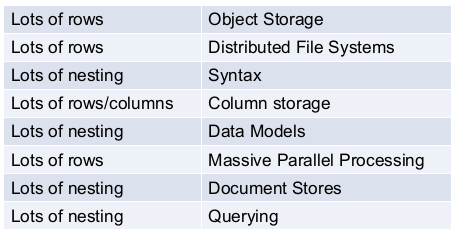
\includegraphics[width=0.8\linewidth]{figures/scaling_up_overview}
		\caption{Data Scale-Up}
		\label{fig:scalingupoverview}
	\end{subfigure}
\end{figure}

\subsection{Transactions}

The good old times of databases: ACID (Atomicity, Consistency, Isolation, Durability). This is a feature of traditional database since it is only achievable on small DBMS. ACID ensures that transactions are correct (e.g. bank transaction: either I receive money and bank updates balance or nothing at all). 

\vspace{-\topsep}
\begin{itemize}
	\setlength{\itemsep}{0pt}
	\setlength{\parskip}{0pt}
	\item Atomicity: Either the entire transaction is applied, or none of it (rollback).
	\item Consistency: After a transaction, the database is in a consistent state again.
	\item Isolation: A transaction feels like nobody else is writing to the database.
	\item Durability: Updates made do not disappear again (changes are persistent).
\end{itemize}
\vspace{-\topsep}

With big data, we drop the ACID principle.

\subsection{Performance}

Optimize for read vs. write intensive:
\vspace{-\topsep}
\begin{itemize}
	\setlength{\itemsep}{0pt}
	\setlength{\parskip}{0pt}
	\item OnLine Transaction Processing	(OLTP):	Write-intensive
	\item OnLine Analytical Processing (OLAP): Read-intensive
\end{itemize}

There is no such thing as "one size fits all" - data shape matters.

\subsection{Data scale-up}

Data can have lots of rows, lots of columns and lots of nesting. For the rest of this lecture, we are concerned with exactly this: scaling up!

\subsection{SQL}

SQL stems from Sequel (Structured Englisch QUEry Language) and is a declarative language.

\newpage

\titlespacing{\subsection}{0pt}{0ex}{0ex}

\section{SQL}

SQL is a family of standards, namely it includes a data definition language for schemas, a data manipulation language for updates and a query language for reads. Note that SQL is case-insensitive.

\subsection{DDL: Data Definition Language}
\vspace{-\topsep}
\begin{figure}[hb!]
	\centering
	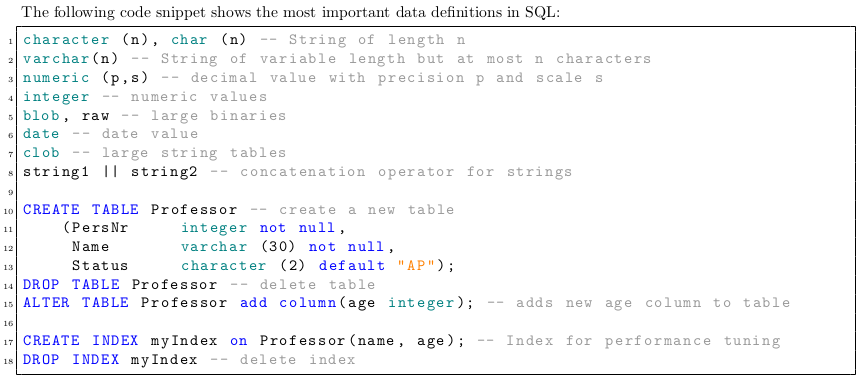
\includegraphics[width=1\linewidth]{figures/sql_1}
	\label{fig:sql1}
\end{figure}
\vspace{-\topsep}

\subsection{DML: Data Manipulation Language}
\vspace{-\topsep}
\begin{figure}[hb!]
	\centering
	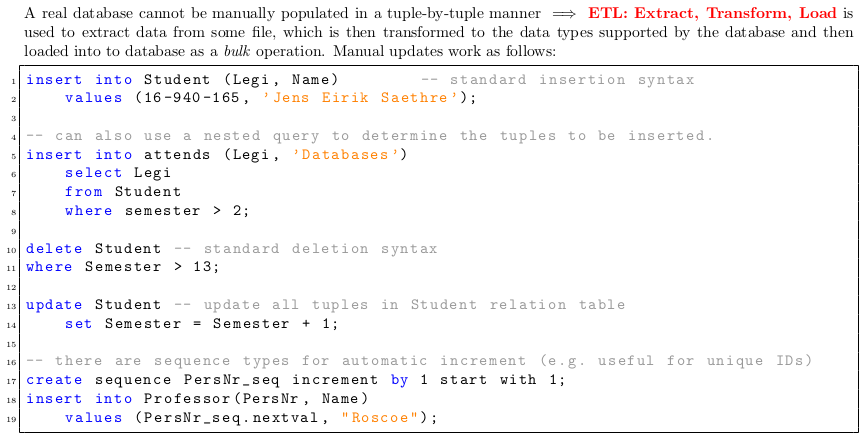
\includegraphics[width=1\linewidth]{figures/sql_2}
	\label{fig:sql2}
\end{figure}
\vspace{-\topsep}

\subsection{Simple Queries in SQL}
\vspace{-\topsep}
\begin{figure}[hb!]
	\centering
	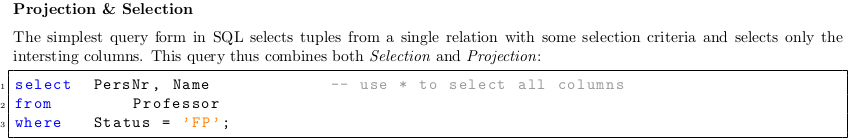
\includegraphics[width=1\linewidth]{figures/sql_3}
	\label{fig:sql3}
\end{figure}
\vspace{-\topsep}

\newpage
\vspace{-\topsep}
\begin{figure}[t!]
	\centering
	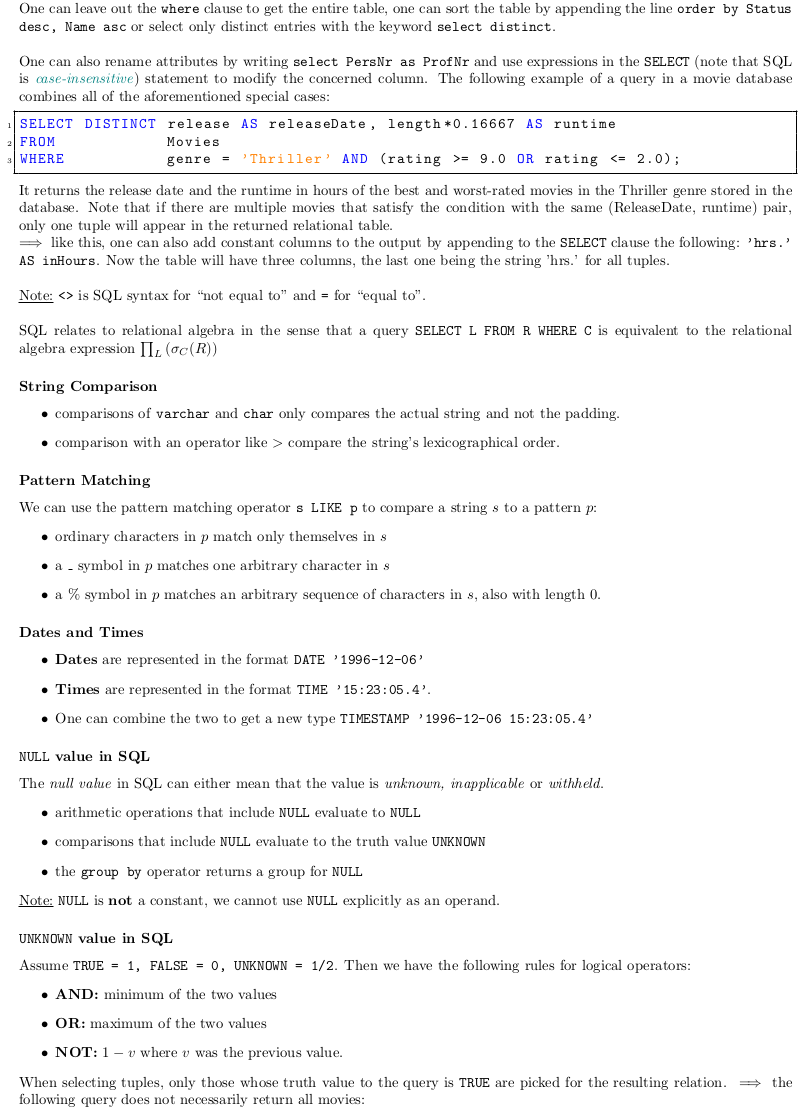
\includegraphics[width=1\linewidth]{figures/sql_4}
	\label{fig:sql4}
\end{figure}
\vspace{-\topsep}

\newpage

\vspace{-\topsep}
\begin{figure}[t!]
	\centering
	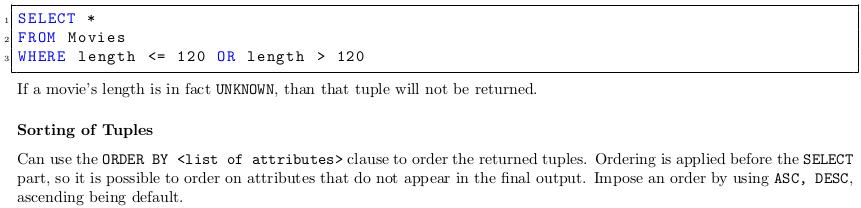
\includegraphics[width=0.95\linewidth]{figures/sql_5}
	\label{fig:sql5}
\end{figure}
\vspace{-\topsep}

\subsection{Queries on multiple Relations}

\vspace{-\topsep}
\begin{figure}[hb!]
	\centering
	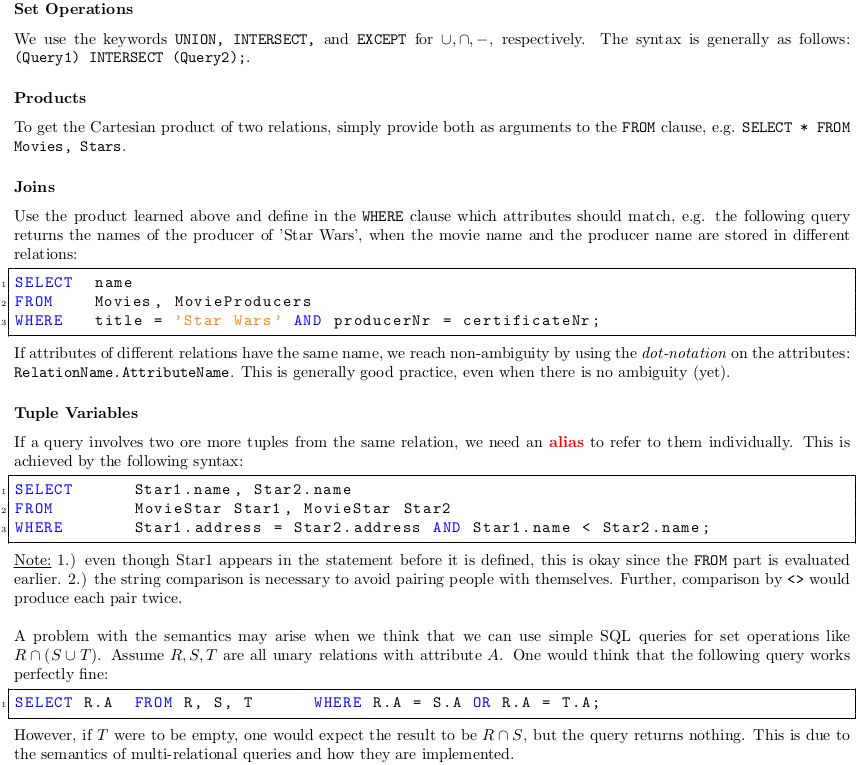
\includegraphics[width=1\linewidth]{figures/sql_6}
	\label{fig:sql6}
\end{figure}
\vspace{-\topsep}

\subsection{Full-Relation Operations}
\vspace{-\topsep}
\begin{figure}[hb!]
	\centering
	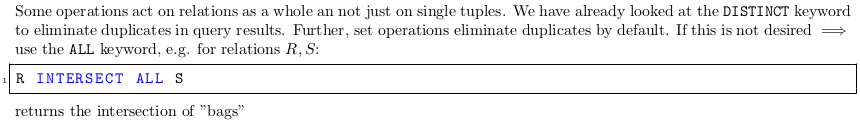
\includegraphics[width=1\linewidth]{figures/sql_7}
	\label{fig:sql7}
\end{figure}
\vspace{-\topsep}

\newpage

\vspace{-\topsep}
\begin{figure}[hb!]
	\centering
	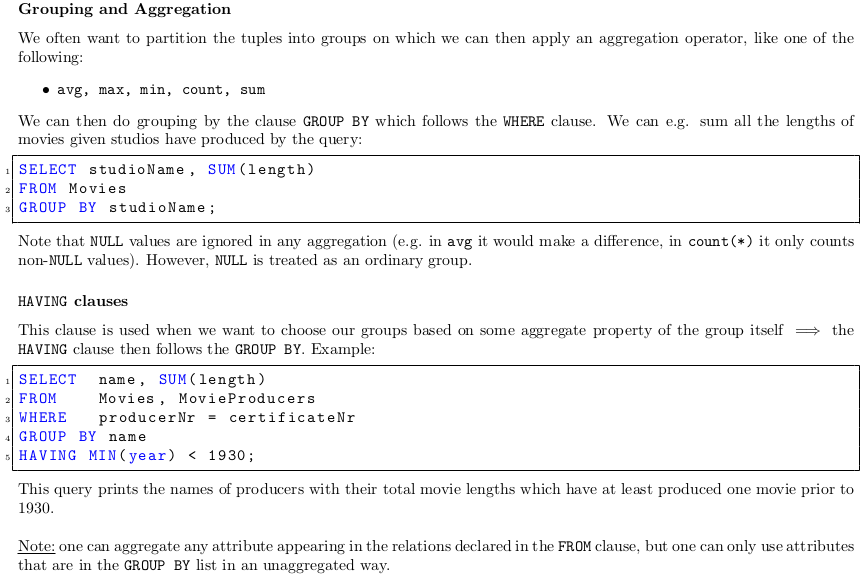
\includegraphics[width=1\linewidth]{figures/sql_8}
	\label{fig:sql8}
\end{figure}
\vspace{-\topsep}

\subsection{Subqueries}

\vspace{-\topsep}
\begin{figure}[hb!]
	\centering
	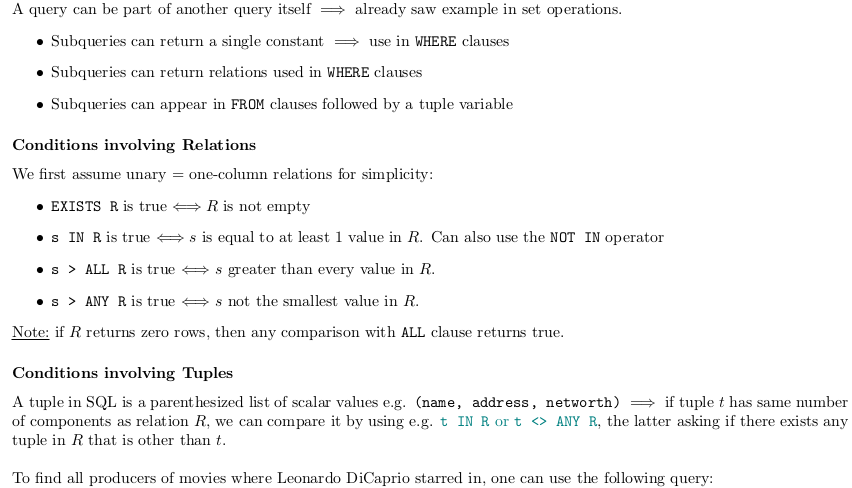
\includegraphics[width=1\linewidth]{figures/sql_9}
	\label{fig:sql9}
\end{figure}
\vspace{-\topsep}

\newpage

\vspace{-\topsep}
\begin{figure}[hb!]
	\centering
	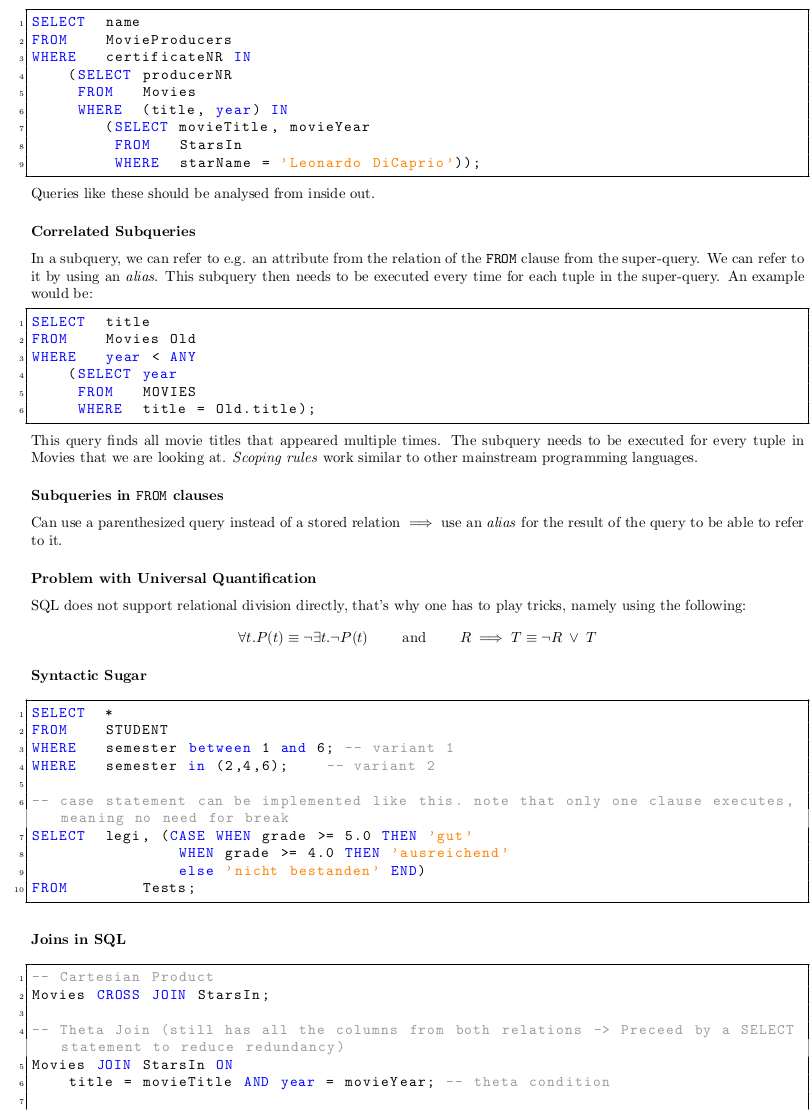
\includegraphics[width=1\linewidth]{figures/sql_10}
	\label{fig:sql10}
\end{figure}
\vspace{-\topsep}

\newpage

\vspace{-\topsep}
\begin{figure}[hb!]
	\centering
	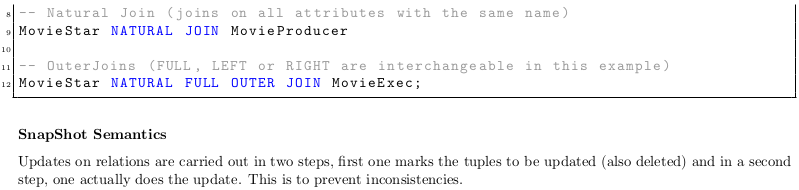
\includegraphics[width=1\linewidth]{figures/sql_11}
	\label{fig:sql11}
\end{figure}
\vspace{-\topsep}

\subsection{Views}

\vspace{-\topsep}
\begin{figure}[hb!]
	\centering
	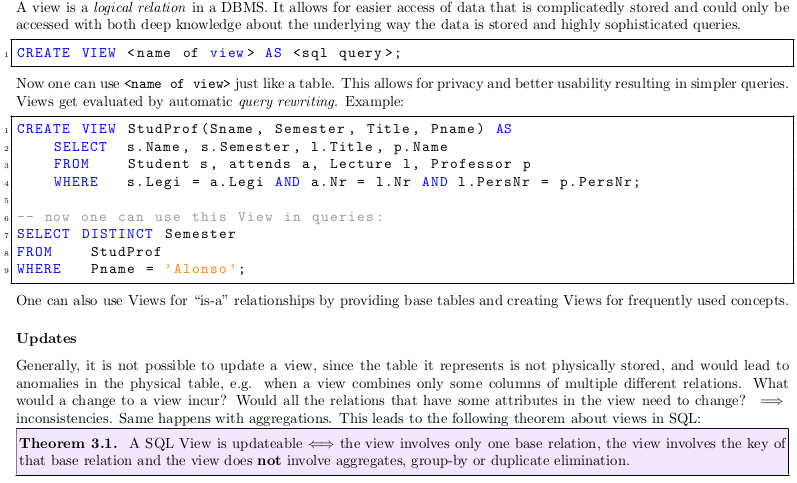
\includegraphics[width=1\linewidth]{figures/sql_12}
	\label{fig:sql12}
\end{figure}
\vspace{-\topsep}

\newpage

\section{Object Storage}

Data needs to be stored somewhere. The common notion nowadays is to just put the data in the cloud - this section describes how to do this.

As we've seen, classic relational databases that fit on a single machine are still very important today - if the data fits in a relational database, you should choose a relational database. However, petabytes of data do not fit on a single machine. We need to somehow break the monolithic relational database down and rebuild while reusing the good parts of relational databases (e.g. SQL language).\\

What can we adapt from relational databases:

\begin{compactitem}
	\item Relational algebra: selection, projection, grouping, sorting, joining
	\item Language: SQL, declarative language, functional language, optimizations, query plans, indices
	\item What is a table made of: table, rows, columns, primary key\\
\end{compactitem}

What we throw out of the window:

\begin{compactitem}
	\item Consistency constraints: Tabular integrity, Domain integrity, Atomic integrity ($1^{st}$ normal form), Boyce-Codd normal form.
	\begin{compactitem}
		\item With NoSQL, we now newly have: Heterogeneous data, Nested data, Denormalized data
	\end{compactitem}
	\item Transactions - ACID: Atomicity, Consistency, Isolation, Durability
	\begin{compactitem}
	\item With NoSQL, we now newly have: Atomic Consistency, Availability, Partition tolerance, Eventual Consistency
	\end{compactitem}
\end{compactitem}

\subsection{The stack}

\begin{figure}
	\centering
	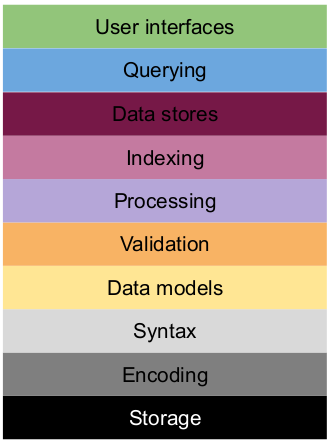
\includegraphics[width=0.2\linewidth]{figures/data_stack}
	\caption{The data stack}
	\label{fig:datastack}
\end{figure}

\begin{compactitem}
	\item \textbf{Storage} - the actual data needs to be physically stored somehow: Local filesystem, NFS, GFS, HDFS, S3, Azure Blob Storage
	\item \textbf{Encoding} - we need to somehow represent and encode data: ASCII, ISO-8859-1, UTF-8, BSON
	\item \textbf{Syntax} - represent data as text: Text, CSV, XML, JSON, RDF/XML, Turtle, XBRL
	\item \textbf{Data models} - provide a level of abstraction over the syntax (only ever dealing directly with syntax would be very tedious):	Tables (Relational model), Trees (XML Infoset, XDM), Graphs (RDF), Cubes (OLAP). All data upwards from the 'data model' level in the stack has the form of tables, trees, graphs, cubes,... \textbf{not} encoded data $\rightarrow$ level of abstraction over data.
	\item \textbf{Validation} - Check that the data is correct (e.g. check that date format is DD-MM-YYYY), data cleaning can be very expensive: XML Schema, JSON Schema, Relational schemas, XBRL taxonomies
	\item \textbf{Processing}: Two-phase processing (MapReduce), DAG-driven processing (Tez, Spark, Flink, Ray),\\ Elastic computing (EC2)
	\item \textbf{Indexing} - make processing faster by building structures: Key-value stores, Hash indices, B-Trees, Geographical indices, Spatial indices
	\item \textbf{Data stores} - the final product: RDBMS (Oracle/IBM/Microsoft), MongoDB, CouchBase, ElasticSearch, Hive, HBase, MarkLogic, Cassandra. \textbf{But} this is not yet a database, just a data store; the data store is still low level, we need a high level language for it to be a database.
	\item \textbf{Querying}: SQL, XQuery, JSONiq, N1QL, MDX, SPARQL, REST APIs
	\item \textbf{User interfaces (UI)} - user doesn't even need to use a query language: Excel,	Access,	Tableau, Qlikview, BI tools, voice assistants (Siri, Alexa,...)
\end{compactitem}

This section talks about the storage.


\subsection{Storage: from a single machine to a cluster}

Data needs to be stored somewhere. Back in the 70s, data was rather limited and we could just store databases locally on a single HDD on a single machine. In a classic file storage, files are organized in a hierarchy (the file system).\\
Typically, a file is made of:

\begin{compactitem}
	\item File metadata: information about the file such as access rights, creation date, etc. File metadata has the data shape \textit{table}.
	\item File content: The actual content is stored in blocks on disk (not just as one large junk). E.g. FFS: files are represented by inodes which point to various data blocks that make up the file.
\end{compactitem}

Issues with local storage:
\begin{compactitem}
	\item Local storage is possible on a local machine and on the LAN (e.g. a NAS). However, local storage is not usable for the WAN - we can't share a local drive with 100s of millions of people. We'd like to find a way to make this possible.
	\item Scaling issues: $10^3$ or even $10^6$ files fit on a local storage. However, we can't fit $10^9$ files on a single machine.\\
\end{compactitem}

\textbf{So how do we make this scale?}

\begin{compactitem}
	\item Throw away the hierarchy and use a \textbf{flat} file system.
	\item Make metadata flexible - don't force metadata to be a table - it can be any data shape.
	\item Make the data model trivial - just assign a name to every object, i.e. an ID for each file, no more structure - essentially a \textbf{key-value store}.
	\item Use commodity hardware - scalability principle: take lots of simple, known instances (i.e. local machine).\\
\end{compactitem}

... and we get Object Storage.\\

\begin{figure}
	\centering
	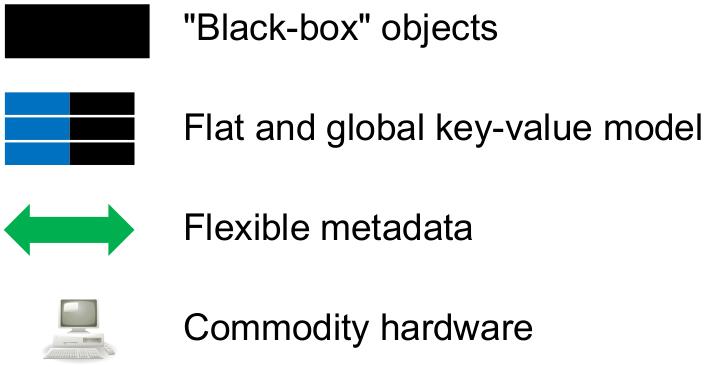
\includegraphics[width=0.25\linewidth]{figures/object_storage}
	\caption{Object storage}
	\label{fig:objectstorage}
\end{figure}

\subsection{Scale}

One single machine is not good enough - how do we scale?

\begin{compactitem}
	\item Approach 1: Scaling \textbf{UP} - more cores, more memory, etc. Scaling up gets extremely expensive very fast (exponentially) - e.g. RAM: 32GB RAM is ok, 64GB RAM is ok, 128GB is still ok, ..., 6TB RAM exists but is exponentially more expensive. 50TB RAM doesn't even exists, would need to be developed.
	\item Approach 2: Scaling \textbf{out} - instead of buying faster, bigger machines, just buy more of the same machine! Scaling up is much more scalable in terms of hardware cost - the cost essentially just increases linearly with the number of machines we buy.
	\item Approach 3: Be smart (this is the first thing you should always do)\\
\end{compactitem}

\subsection{Scaling out}

\textbf{Data centers:} All these single machines need to live somewhere - in a data center. A data center is essentially a collection of \textit{1'000 - 100'000 servers}, each of which has \textit{1-100 cores}. Having more than 100'000 servers in a single DC is hard because of coordination but mainly due to energy consumption for power and cooling. Each server has \textit{1-20TB of storage} and \textit{16GB - 6TB of RAM}. Servers are connected and the network achieves \textit{1-100 GB/s throughput} - high network throughput is very important since servers send data among each other. Servers have the form of \textit{rack servers} which allows to efficiently stack them in racks. A \textit{rack unit} (RU) refers to the height of a rack server. A DC has multiple racks. Racks are modular - they can contain servers, storage, routers etc.\\

\textbf{Take away message: how to scale out?} Simplify the model, buy (lots of) cheap hardware, remove schemas.

\newpage

\subsection{Amazon S3}

\begin{figure}
	\centering
	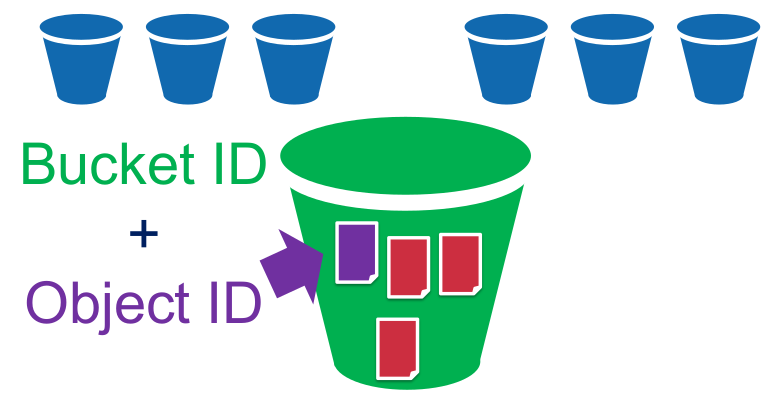
\includegraphics[width=0.2\linewidth]{figures/s3_buckets}
	\caption{S3 model}
	\label{fig:s3buckets}
\end{figure}

Amazon's S3 model is very simple, it's essentially: \textit{objects in buckets}. S3 has no tables, cubes,... and no nesting (no buckets in buckets). We have many buckets and each bucket has a \textit{bucket ID}. Each object inside a bucket has an \textit{object ID}. Having buckets makes things cleaner and makes it easy to assign them to machines. An object can be anything (picture, video, etc.) and every object can be accessed by the tuple $(bucket\_id, object\_id)$. The \textit{maximum object size is 5TB} and we can have up to 100 buckets per account (more upon request).

\textbf{Service level agreement (SLA):} SLA assures the quality of the service, e.g. 99.999999999\% durability (loss of 1 in $10^{11}$ objects in a year) and 99.9\% availability (1h/year downtime). Very high SLAs are \textit{very} hard to achieve (e.g. 99.99999\% SLA) corresponds to 4seconds/year outage - almost impossible. Amazon has a different approach to SLAs: response time $<$ 10ms in 99.9\% of the cases.

\subsection{APIs}

API (application programming interface) is a set of rules and mechanisms by which one application or component interacts with the others. API can return data that you need for your application in a convenient format (e.g. JSON or XML). We need to somehow interact with the objects:

\begin{compactitem}
	\item Driver (Java Database Connectivity (JDBC)...) for various programming languages
	\item SOAP
	\item REST (lightweight version of SOAP)\\
\end{compactitem}

\subsection{Properties}

We want certain properties for databases. But:\\
\textbf{CAP theorem:} One cannot achieve consistency, availability and partition tolerance all at the same time.\\
\textit{Proof:} Imagine a system (e.g. bank) that is in a partitioned state. At right that time, someone requests the service (e.g. ATM). The system can now either serve the user - giving up partition tolerance (service will change state which won't be propagated globally due to the partition) \textit{OR} the system cannot serve the user - giving up availability.

\begin{compactitem}
	\item (Atomic) Consistency:	All nodes see the same data.
	\item Availability:	It is possible to query the database at all times.
	\item Partition tolerance: The database continues to function even if the network gets partitioned.\\
\end{compactitem}

\subsection{REST APIs}

REST (representational state transfer) provides data presentation for a client in the format that is convenient for it and is typically based on the HTTP protocol. REST is not a standard or protocol, it is an approach to or architectural style for writing API! REST is based on the client-server model.

HTTP is used to request resources over a network. Resources are addressed through a URI (uniform resource identifier) e.g. \textit{http://www.ethz.ch/, http://www.mywebsite.ch/api/collection/foo/object/bar, mailto:sheldon.lee.cooper@ethz.ch}.

Let's dissect a URI: http://www.mywebsite.ch/api/collection/foo/object/bar?id=foobar\#head

\begin{compactitem}
	\item http: gives the protocol
	\item www.mywebsite.ch: the authority (domain)
	\item api/collection/foo/object/bar: the path (often this is the exact path on the server, e.g. for static websites)
	\item ?id=foobar: The query
	\item \#head: The fragment (directly jumps to specific part of the page)
\end{compactitem}

\textbf{HTTP methods}

\begin{compactitem}
	\item GET: get the resource (side-effect free)
	\item PUT: create a new resource and store it (idempotent)
	\item DELETE: delete a resource (if you send DELETE then GET on same object $\rightarrow$ 404 page not found)
	\item POST: update the corresponding resource with information provided by the client, or create this resource if it does not exist (not idempotent)\\
\end{compactitem}

All requests you make have their HTTP status codes. There are a lot of them and they are divided into 5 classes. The first number indicates which of them a code belongs to:

\begin{compactitem}
	\item 1xx - informational
	\item 2xx - success
	\item 3xx - redirection
	\item 4xx - client error
	\item 5xx - server error
\end{compactitem}


\subsubsection{S3}

REST with S3: buckets and objects: http://\textit{bucket}.s3.amazonaws.com/\textit{object-name}

\textbf{S3 REST API:}

\begin{compactitem}
	\item Bucket: \{PUT, DELETE, GET\} bucket
	\item Object: \{PUT, DELETE, GET\} object\\
\end{compactitem}

\textbf{Folders: is S3 a file system?}
The physical file system in S3 is flat - there are no folders/hierarchies. But we can simulate a hierarchy by naming objects as if they were in a hierarchy. This will be displayed as a hierarchy. Thus, on the logical level (browsing), S3 looks like a hierarchical file system but on the physical level (object keys) it's really a flat file system. (Again, it is important to distinguish between the physical and logical part).\\
The objects would then have names such as \textit{/food/fruits/orange, /food/vegetables/tomato} which simulates the hierarchy.

S3 can host various things such as static websites or datasets. Datasets are just lots different files put into objects. This is different from relational DBs where we split data by having different tables for different instances (e.g. order, customer table). Here we don't have a file for order and a file for customer.\\

\subsection{More on storage}

\textbf{Replication}: We want fault tolerance (faults happen). This can be achieved by replication (if you replicate the file, loosing it totally is less likely). Faults can happen locally (node failure) and regionally (natural catastrophe).
\begin{compactitem}
	\item Local fault: replicate over multiple local machines
	\item Regional fault: replicate over multiple DCs in various regions. This gives us better resiliency to natural catastrophes and better latency.
\end{compactitem}

Cloud providers offer different storage classes, trading availability for cost:

\begin{compactitem}
	\item Standard: High availability
	\item Standard - Infrequent Access: Less availability, Cheaper storage, Cost for retrieving
	\item Amazon Glacier: Low-cost, Hours to GET\\
\end{compactitem}

\subsection{Azure Blob Storage}

Azure blob storage is different from S3:

\begin{tabular}{|c|c|c|}
	\hline 
	& S3 & Azure \\ 
	\hline 
	Object ID & Bucket + Object & Account + Container + Blob \\ 
	\hline 
	Object API & Blackbox & Block (like bucket)/Append (for logs)/Page (for VMs)\\ 
	\hline 
	Limit & 5TB & 4.78 TB (block), 195 GB (append),	8TB (page) \\ 
	\hline
\end{tabular}\\

Azure thus has one more layer of indirection: account, container, blob. Further, Azure doesn't view an object as a blackbox, it let's you see inside and differentiate between 3 types of blobs: block, append, page. The account name maps to a virtual machine which is responsible for my data. The partition name is a chunk of data and the stream layer streams data over to me. In the Azure datacenter (i.e. one storage stamp) we have 10-20 racks, each with 18 storage nodes. This totals to 30PB ($= 30*10^{15} bytes$) per datacenter - over the whole world, Azure reaches an exabyte range of storage. Azure keeps the usage of the datacenter below 70-80\% storage capacity since dealing with full storage is annoying.\\

\textbf{Storage replication:}

\begin{compactitem}
	\item Intra-stamp replication (synchronous): Replication within the streaming layer (i.e. within the same location (data center)).
	\item Inter-stamp replication (asynchronous): Replication between different partition layers (i.e. between different locations (data centers))\\
\end{compactitem}

\textbf{Location services:} Azure has globally distributed data centers for load balancing and latency optimization. The location service works as follows:

\begin{compactenum}
	\item Location service sends request with account name to DNS server.
	\item DNS server returns a virtual IP that is mapped to the account name. The virtual IP points to a primary storage stamp and also to a backup storage stamp.
\end{compactenum}

\vspace{-\topsep}
\begin{figure}[hb!]
	\centering
	\begin{subfigure}[t]{.5\textwidth}
		\centering
		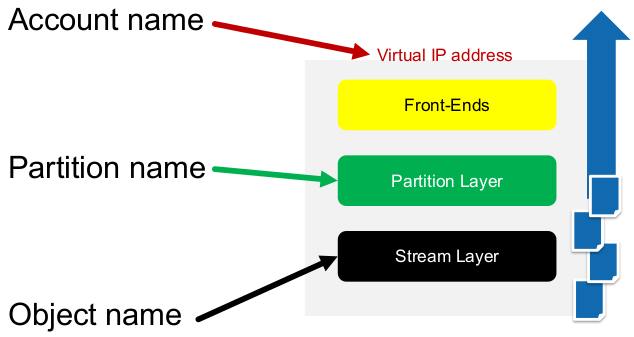
\includegraphics[width=0.5\linewidth]{figures/azure_storage_stamp}
		\caption{Azure storage stamp}
		\label{fig:azure_storage_stamp}
	\end{subfigure}%
	\begin{subfigure}[t]{.5\textwidth}
		\centering
		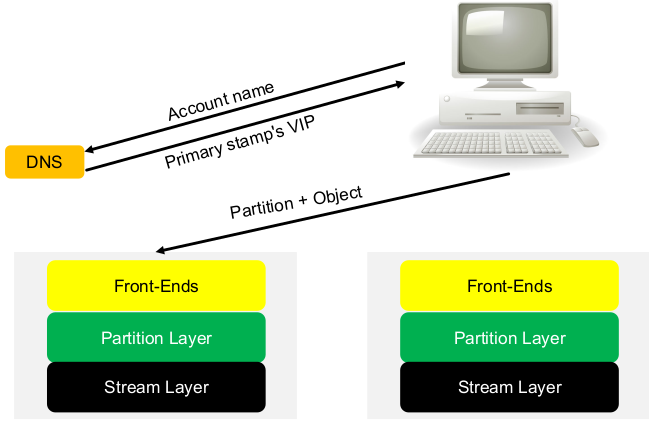
\includegraphics[width=0.6\linewidth]{figures/azure_location_services}
		\caption{Azure location services}
		\label{fig:azure_location_services}
	\end{subfigure}
\end{figure}

\textbf{Stream Layer:} Stores the bits on disk and is in charge of distributing and replicating the data across many servers to keep data durable within a storage stamp. Can be thought of as a distributed file system layer within a stamp. The default replication policy is to keep 3 replicas within a storage stamp.\\
\textbf{Partition Layer:} Built for (a) managing and understanding higher level data abstractions (Blob, Table, Queue), (b) providing a scalable object namespace, (c) providing transaction ordering and strong consistency for objects, (d) storing object data on top of the stream layer, and (e) caching object data to reduce disk I/O.\\
\textbf{Front-End Layer:} Set of stateless servers that take incoming requests.\\


\subsection{Mindsets}

Amazon and Azure have different mindsets in their cloud services:

\begin{compactitem}
	\item Amazon mindset: Amazon thinks a lot in terms of modules. They have ~200 different services they offer (S3, domain management, AWS,...) $\rightarrow$ a lot of small services that each do one particular thing.
	\item Azure mindset: Azure has bigger services that do more $\rightarrow$ fewer services that do several things.\\
\end{compactitem}

\section{Distributed file systems}

Where does data come from?

\begin{compactitem}
	\item Raw data: sensors, measurements, events, logs (e.g. CERN sensor measurements)
	\item Derived data: aggregated data, intermediate data (e.g. computational results on sensor measurements)
\end{compactitem}

Big Data isn't big data - there are different cases:

\begin{compactitem}
	\item \textbf{A	huge amount of large files} (billions of TB files): This is what S3 is $\rightarrow$ lots of files, but single files are not extremely big, just large (e.g. 5TB for S3).\\
	$\rightarrow$ Object storage + Key-value model
	\item \textbf{A large amount of huge files} (millions of PB files): We need something new for this...\\
	$\rightarrow$ Block storage + file system
\end{compactitem}

Google had just this idea: have a FS that looks and feels like a normal file system \textit{but} lives on a distributed cluster. Google went on and developed GoogleFS.

\subsection{Fault tolerance and robustness}

We have different paradigms for fault tolerance:

\begin{compactitem}
	\item Local disk: the disk \textit{might} fail, we can just keep a backup \textit{in case.}
	\item Cluster with 100s to 10'000s machines: nodes \textit{will} fail ($P[\text{at least one node fails
	}] = 1-(1-p)^n$, with $n$: \#nodes, $p$: failure probability of a single node). We thus need a stronger property for clusters, we can't restore from backups every single day.
\end{compactitem}

How to achieve fault tolerance and robustness on clusters:

\begin{compactitem}
	\item Fault tolerance (system keeps working under faults)
	\item Automatic Recovery (can't recover manually with lots of disks)
	\item Error detection (know about failed disks)
	\item Monitoring (keep an overview over what's working)
\end{compactitem}

\subsection{File system specifications}

\textbf{File read/update model:}

\begin{compactitem}
	\item Random access (can read at any position in a file): this is hard to do in clusters
	\item Sequential access (scan the file from the beginning (reading)/ append to file (update): this is easier for distributed clusters, that's why (most) do it like this
\end{compactitem}

Appends: You can only append, can't go back and change something. This is suitable for sensor data, logs and also intermediate data. \textbf{Note:} Since we have a distributed FS, we have 100s of clients in parallel reading/writing $\rightarrow$ we want atomicity. HDFS implements a single-writer, multiple-reader model.

\textbf{Performance requirements:}

Our top priority is throughput (how fast do you read/write). Secondary, we want latency (time until we start reading/writing).

Remember: we have a huge discrepancy between storage capacity, throughput and latency. Over the last 60 years, storage capacity improved by 200'000'000'000, throughput improved by 10'000 and latency improved by 8. The solution for the capacity-throughput discrepancy is to parallelize. The solution for the throughput-latency discrepancy is to do batch-processing.\\
Latency is usually not a problem in big data since the data is so large, the read/write time dominates the latency.\\
A similar discrepancy between throughput and latency can be observed in websites. In the 90s, a website started loading slowly, elements appeared one after another $\rightarrow$ throughput was the issue. Today, website is blank for ~1s and then the whole website appears $\rightarrow$ latency is the issue.

\subsection{Hadoop}

Hadoop is primarily:

\begin{compactitem}
	\item Distributed File System (HDFS) (inspired by Google's GFS)
	\item MapReduce (inspired by Google's MapReduce)
	\item Wide column store (HBase) (inspired by Google's BigTable)
\end{compactitem}

\subsection{Distributed file systems: the model}

Again, rememeber data independence: separate the logical model from the physical model.

\textbf{File system (logical model):} In distributed file systems, we have a \textbf{file hierarchy} (unlike the key-value model in object storage which is flat).

\textbf{Block storage (physical storage):} In distributed file systems, we have block storage (unlike object storage (S3) where we have a blackbox model).\\
\textbf{Terminology}: HDFS: Block, GFS: Chunk.
We thus have a hierarchy of files where each file is associated with a chain of blocks.\\

\textbf{Why blocks?} 1) The files are bigger than a disk (PBs), there is no way the files fit on a single machine $\rightarrow$ need blocks. 2) Simple level of abstraction and blocks are easy to distribute over multiple nodes.

\textbf{Block size:} Every file is a multiple of blocks. In a simple file system, we have a block size of 4kB $\rightarrow$ good size for local machines, good compromise. However, in distributed file systems, things are different: blocks travel over the network and we have very large (PB) files. Due to the throughput-latency discrepancy, we want larger blocks (for small blocks, the latency would outweigh the transfer time). Further, large blocks lead to less blocks being read per file. The block size in distributed file systems is \textbf{64MB - 128MB}. This is a good compromise - not too many blocks for big files, but also small enough to have several blocks on one machine.\\

\subsection{HDFS Architecture}

\begin{figure}[hb!]
	\centering
	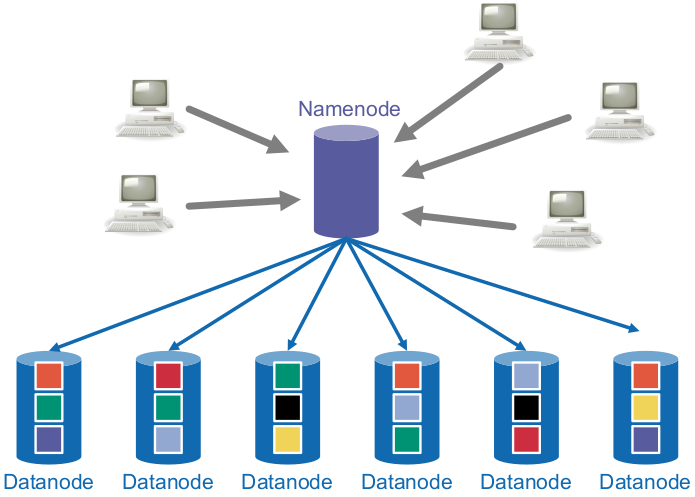
\includegraphics[width=0.3\linewidth]{figures/hdfs_architecture}
	\label{fig:hdfsarchitecture}
\end{figure}


We need to connect the many machines somehow. One possible way would be peer-to-peer, but this is not ideal. HDFS uses a master-slave architecture: the namenode (has the names of the files) is the master and the datanodes (have the actual data) are the slaves.\\
How it works from the file perspective: The file is divided into 128MB chunks. The chunks are then stored in datanodes. Each chunk is replicated 3 times (the \# of replicas can be specified).

\subsubsection{Namenode}

The namenode will be concurrently accessed by multiple clients. The namenode is responsible for all system-wide activity:

\begin{compactitem}
	\item File namespace (+Access Control): keep track of hierarchy of files. This is actually rather small (hierarchy doesn't contain the actual file data, just the hierarchy).
	\item File to block mapping: every file is associated with a list of blocks. The namenode keeps track of the mapping $file \rightarrow \{blocks\}$.
	\item Block location: for every block, the namenode needs to know on which 3 (default) datanodes the block is stored.
\end{compactitem}

\subsubsection{Datanode}

A datanode is a machine with multiple local disks. Blocks are stored on these local disks. Datanodes are responsible for failure detection. Each datanode has its own local view over its disks - proximity to hardware facilitates disk failure detection. Each block has a \textit{block ID (64bit)}. It is also possible to access blocks at a subblock granularity to request parts of a block.

\subsubsection{Communication}

\textbf{Client protocol:} The client protocol handles \textit{client-namenode} communication. Clients sends metadata operations (e.g. create directory, delete directory, write file, append to file, read file,
delete file) and the namenode responds with the datanode location and the block IDs.\\

\textbf{DataNode protocol:} The datanode protocol handles \textit{datanode-namenode} communication. The datanode always initiates the connection. The following types of datanode-namenode communication exist:

\begin{compactitem}
	\item registration
	\item heartbeat: datanode tells namenode every 3s that it's still alive
	\item blockreport: every 6h, datanode sends full list of blocks (not the contents of the blocks) to the namenode
	\item blockReceived\\
\end{compactitem}

\textbf{Data transfer protocol:} The data transfer protocol handles \textit{client-datanode} communication and is used by clients to read actual block content. The client knows which datanode to contact for a given block - it got that information from the namenode.\\
Client reads a file:

\begin{compactenum}
	\item Client asks namenode for file
	\item Namenode sends block location (multiple datanodes for each block, sorted by distance) to client
	\item Client reads data from datanode via input stream\\
\end{compactenum}

Client writes a file:

\begin{compactenum}
	\item Client sends create to namenode
	\item Namenode sends datanodes (all replicas) for first block
	\item Client organizes pipeline by contacting one datanode and tells the datanode which other datanodes to forward the data to
	\item Client then sends the data over to the datanode
	\item Datanode sends Ack to client
	\item Namenode sends datanodes for second block (writing happens block by block, for every block the client contacts a datanode which will also forward to other datanodes (note: if the blocks were very small, this would have large overhead))
	\item ...
	\item Client sends close/release lock
	\item Datanodes check with namenode for minimal replication (datanode protocol)
	\item Namenode sends Ack to client
	\item Namenode can tell datanodes to replicate further asynchronously
\end{compactenum}

This block-by-block writing is all done simultaneously under DFSOutputStream (streaming through), checksums are used to provide data integrity. Clients write by obtaining leases on files. If a client does not release a lease after writing, after the expire of a hard limit, the NameNode assumes the client quit.

\begin{figure}[t!]
	\centering
	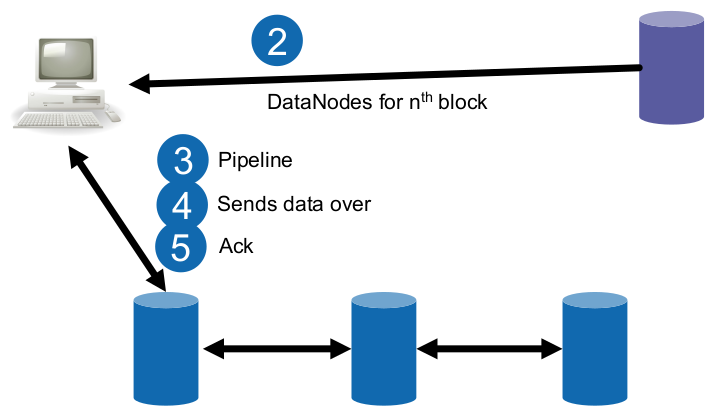
\includegraphics[width=0.4\linewidth]{figures/hdfs_client_write}
	\caption{Client writes a file to HDFS}
	\label{fig:hdfsclientwrite}
\end{figure}

\newpage

\subsection{Replicas}

The number of replicas per file can be specified (default: 3). The replicas need to be placed in a smart way. Have the topology of a data center in mind: we have a cluster consisting of multiple racks, each rack consisting of multiple nodes. We add a notion of distance between nodes $D(A,B)$.\\
The replicas are placed as follows:

\begin{compactitem}
	\item Replica 1: same node as client (or random), rack A\\
	(Note: in practice, the actual client is not on my laptop but on a node in the data center and my laptop connects to it. The 1st replica goes on that node because it's very efficient).
	\item Replica 2: a node in a different rack B (put in a different rack from 1st replica - racks can fail)
	\item Replica 3: in same rack B but on a different node
	\item Replica 4 and beyond: random, but if possible:
	\begin{compactitem}
		\item at most one replica per node
		\item at most two replicas per rack\\
	\end{compactitem}
\end{compactitem}

What if we placed replicas 1\&2 on the same rack? If you always put the first two replicas on the same rack as my client node $\rightarrow$ 2/3 of replicas of all blocks written by the client will be on the same rack (the client stays on the same node) $\rightarrow$ worse replication factor.\\

We could also put all first 3 replicas on 3 different racks, but this would need more data being sent between racks (takes longer).

\textbf{Distance:} HDFS estimates the network bandwidth between two nodes by their distance. The distance from a node to its parent node is assumed to be one. A distance between two nodes can be calculated by summing up their distances to their closest common ancestor. A shorter distance between two nodes means that the greater bandwidth they can utilize to transfer data. The distance between two nodes a, b in racks A, B is:\\
$d(A,B) = \text{\#hops to TOR switch A + \#hops to cluster switch + \#hops to TOR switch B + \#hops to node b}$\\

\subsection{Performance and availability}

The NameNode is responsible for file namespace, file-block mapping, block locations and is a single point of failure. We want the file namespace and file-block mapping to persist; the block locations don't need to persist since datanodes will tell us the blocks they have. HDFS thus puts the namespace file and an edit log onto persistent storage (edit log allows to not rebackup the whole hierarchy and mapping, only the things that change). We further also backup the persistent storage with the namespace file and the edit log to shared drives/ backup drives/ etc.

What if the namenode fails? We need to start it up again:

\begin{compactitem}
	\item Restore the initial hierarchy/ block mapping and then 'play' the edit log and apply changes to the file systems (restore last logged version)
	\item Receive the block locations from the block reports, which are periodically sent by the datanode (can also be manually requested)
\end{compactitem}

This startup takes ~30min. Can we do better?

\begin{compactitem}
	\item Checkpoints: periodically play the edit log and reconstruct a more recent namespace file. This way, we don't have to replay the \textit{whole} edit log upon failure.
	\item High Availability (HA): Standby NameNodes. Have standby machines that keep the exact same state and immediately take over in case the active namenode crashes.
	\item Federated DFS: dedicated namenodes for different top directories.
\end{compactitem}

\subsection{Using HDFS}

We can interact with HDFS as with a normal POSIX file system:

\vspace{-\topsep}
\begin{verbatim}
$ hadoop fs -ls
$ hadoop fs -cat /dir/file
$ hadoop fs -rm /dir/file
$ hadoop fs -mkdir /dir2
\end{verbatim}

HDFS Shell: upload and download

\vspace{-\topsep}
\begin{verbatim}
$ hadoop fs -copyFromLocal localfile1 localfile2 /user/hadoop/hadoopdir
$ hadoop fs -copyToLocal /user/hadoop/file localfile
\end{verbatim}\\
\vspace{-\topsep}

\textbf{Populating HDFS:}
\begin{compactitem}
	\item Apache Flume: Collects, aggregates, moves log data (into HDFS)
	\item Apache Sqoop: Imports from a relational database\\
\end{compactitem}

\subsection{Reading: The Hadoop Distributed File System \cite{shvachko2010hadoop}}

\begin{compactitem}
	\item All servers are fully connected and communicate with each other using TCP-based protocols.
	\item DataNodes in HDFS do not use data protection mechanisms such as RAID - they use replication.
	\item Files and directories are represented on the NameNode by inodes, which record attributes like permissions, modification and access times, namespace and disk space quotas. The file content is split into large blocks (typically 128 megabytes, but user selectable file-by-file) and each block of the file is independently replicated at multiple DataNodes (typically three, but user selectable file-by-file).
	\item Each block replica on a DataNode is represented by two files in the local host’s native file system. The first file contains the data itself and the second file is block’s metadata including checksums for the block data and the block’s generation stamp.
	\item Unlike conventional file systems, HDFS provides an API that exposes the locations of a file blocks. This allows applications like the MapReduce framework to schedule a task to where the data are located, thus improving the read performance.
	\item An application adds data to HDFS by creating a new file and writing the data to it. After the file is closed, the bytes written cannot be altered or removed except that new data can be added to the file by reopening the file for append. HDFS implements a single-writer, multiple-reader model. The HDFS client that opens a file for writing is granted a lease for the file; no other client can write to the file. 
	\item The BackupNode can be viewed as a read-only NameNode. It contains all file system metadata information except for block locations. It can perform all operations of the regular NameNode that do not involve modification of the namespace or knowledge of block locations. Use of a BackupNode provides the option of running the NameNode without persistent storage, delegating responsibility for the namespace state persisting to the BackupNode.
	\item HDFS generates and stores	checksums for each data block of an HDFS file. Checksums are
	verified by the HDFS client while reading to help detect any corruption caused either by client, DataNodes, or network. When a client creates an HDFS file, it computes the checksum sequence for each block and sends it to a DataNode along with	the data.
\end{compactitem}


\section{Syntax}

Now, we can store data - both structured and unstructured. But: how do the files of data actually look like?

\subsection{Introduction}

Remember: we have data shapes text, trees, tables, cubes and graphs. In this section, we are concerned with the layers \textit{Encoding, Syntax} of the data stack as given in figure \ref{fig:datastack}. The Syntax stack is:

\begin{compactitem}
	\item Text: just text (i.e. the characters)
	\item Table: CSV
	\item Tree: XML, JSON
	\item Graph: RDF/XML, Turtle
	\item Cube: XBRL
\end{compactitem}

\textbf{Semi-Structured Documents}

\begin{compactitem}
	\item Structured: tables
	\item Semi-structured: trees (JSON, XML)
	\item Unstructured: text
\end{compactitem}

Why do we need syntax? Well-formedness: One syntax = one language, decide whether $D \in L$\\


\textbf{The denormalizing road from SQL to NoSQL:}

\begin{compactitem}
	\item Relational database: Homogeneous collection of flat items. Homogeneous meaning that on every row has the same columns and every row has some value for every column (even if null)
	\item Document store: Heterogeneous collection of arborescent items. Heterogeneous meaning that we have missing fields for some data points, you can even have type mismatch for same header in different data points.	
\end{compactitem}

\subsection{CSV (tables)}

In CSV (Comma separated values), we essentially have rows of text, where the top row is a headers row and all following rows are data rows where values are separated by commas. This is very easy - but it works, can have billions of rows. Note: there is an RFC for CSV, but in practice there are multiple 'flavors' of CSV (e.g. how do you escape commas).

\begin{figure}[hb!]
	\centering
	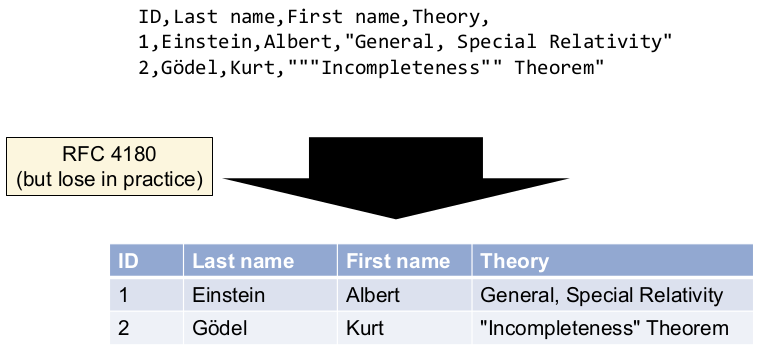
\includegraphics[width=0.4\linewidth]{figures/csv}
	\label{fig:csv}
\end{figure}

\textbf{Remember:} In big data, we break several paradigms from relational databases:

\begin{compactitem}
	\item $1^{st}$ normal form (atomic integrity): no tables in tables
	\item Boyce-Codd Normal Form: have plenty of small tables that do one thing instead of one big table
\end{compactitem}

Relational databases are highly normalized whereas in big data we have data denormalization (NoSQL). A highly normalized DB should be write-intensive and should avoid update anomalies. A highly denormalized DB should be read-intensive and should avoid joins.\\
Nesting (i.e. tables in tables) is \textit{not} possible with CSV.

\subsection{JSON}

JSON is a syntax like CSV but it's based on tuples and we repeat the headers in each new object. Syntax:

\vspace{-\topsep}
\begin{verbatim}
{
"product" : "Phone",
"price" : 800,
"quantity" : 1
}
\end{verbatim}
\vspace{-\topsep}

JSON can represent a normal table (collection of tuples) \textit{but} also nestedness (collection of tuples in tuples). CSV can't do this, in CSV we can only separate single values by comma.\\
\textbf{JSON data types:}

\begin{compactitem}
	\item Strings: \verb|"foo"| (\textit{has} to be double quotes), escaping is possible: \verb|"foo\nbar\u005f"|
	\item Number: \verb|3.1414, -1.2345E+5|
	\item Boolean: \verb|true, false|
	\item Null: \verb|null|
	\item Array: list of anything you want
	\begin{verbatim}
	  [ 3.1414, true, "This is a string", {"foo": false}, null ]
	\end{verbatim}
	\item Object: key-value store (key must be a string, value can be any data type)
	\begin{verbatim}
	  {
	    "foo": 3.14159265368979,
	    "bar": true,
	    "str": "This is a string",
	    "obj": { "school" : "ETH"},
	    "Q": null
	  }
	\end{verbatim}	
\end{compactitem}

\textbf{JSON well-formedness:}

\begin{compactitem}
	\item Keys need to be strings (i.e. require double-quotes "")
	\item Keys (should syntactically but really:) need to be distinct
	\item No backslashes in strings! (need to escape \textbackslash\textbackslash)\\
\end{compactitem}

\subsection{XML}

XML, the Extensible Markup Language, is a W3C-endorsed standard for document markup. XML is really similar to JSON but much more complex. Syntax:

\begin{compactitem}
	\item XML Element: \verb|<foo>[more XML]</foo>|, \verb|<bar/> = <bar></bar>|\\
	\verb|<foo>| is the opening tag, \verb|</foo>| is the closing tag, \verb|[more XML]| is the element's content.\\
	 \verb|<bar/>| is an empty tag. Tag names are \textit{case-sensitive}.
	\item XML Attribute: \verb|<a attr="value"/>|\\
	Key-value pair. Keys can't be repeated in an element. Key: not quoted, value: \textit{must} be quoted (single or double quotes).
	\item XML Text: \verb|<a>This is text</a>|
	\item Text declaration: \verb|<?xml version="1.0" encoding="UTF-8"?>|
	\item Comments: \verb|<!-- I need to verify and update these links when I get a chance. -->|\\
	The double hyphen \verb|--| must not appear anywhere inside the comment until the closing \verb|-->|. In particular, a three-hyphen close like \verb|--->| is specifically forbidden.
	\item Processing Instructions: XML provides processing instructions as an alternative means of passing information to applications that may read the document. A processing instruction begins with \verb|<?| and ends with \verb|?>|. Immediately following the \verb|<?| is an XML name called the target (the name of the application for which this processing instruction is intended or possibly just an identifier for the processing instruction).\\
	example: \verb|<?php [PHP code] ?>|
	\item XML Declaration: XML documents should (but do not have to) begin with an XML declaration.\\
	\verb|<?xml version="1.0" encoding="ASCII" standalone="yes"?>|
\end{compactitem}

\textbf{XML well-formedness:}

\begin{compactitem}
	\item There can only be \textit{one} top element (root element), i.e. can't have:
	\begin{verbatim}
	  <?xml version="1.0" encoding="UTF-8"?>
	  <foo/>
	  <bar/>
	\end{verbatim}
	\item Can't have text outside of top element
	\item Can't have an element inside an element tag. Only between tags is possible.
	\item Can't have same key twice in the same element
	\item Need to respect nesting order of opening and closing tags (like parenthesis order)
	\item No \verb|<| in text (need to escape) - confuses the parser
\end{compactitem}

\begin{figure}[hb!]
	\centering
	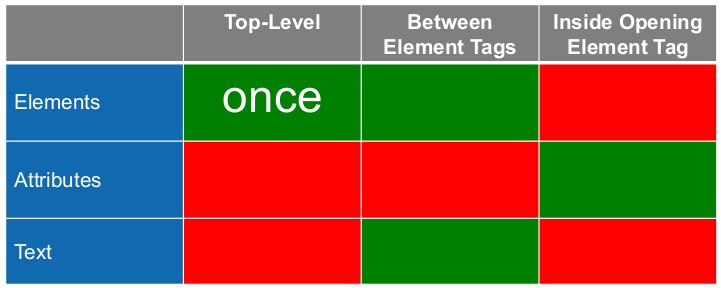
\includegraphics[width=0.4\linewidth]{figures/xml_syntax}
	\caption{What Appears Where?}
	\label{fig:xmlsyntax}
\end{figure}

\textbf{Escape characters (XML: Entity References)}

\begin{compactitem}
	\item \verb|<|: \verb|&lt;|
	\item \verb|>|: \verb|&gt;|
	\item \verb|'|: \verb|&apos;| (Note: single quote inside double-quotes string is ok)
	\item \verb|"|: \verb|&quot;|
	\item \verb|&|: \verb|&amp;|
\end{compactitem}

All these characters need to be escaped. Special characters can also be inserted (see XML character references).\\

\textbf{XML names:} XML names may contain any alphanumeric character. This includes A-Z, a-z, 0-9, non-English letters, numbers, and ideograms, such as ö, ç, $\Omega$, the  three punctuation characters '\_', '-', '.'. XML names may not contain other punctuation characters such as quotation marks, apostrophes, dollar signs, carets, percent symbols, and semicolons. The colon is allowed, but its use is reserved for namespaces.\\
XML names can't start with numbers and we can't have \verb|<| in a name. All names beginning with the string “XML” (in any combination of case) are reserved for standardization in W3C XML-related specifications.\\

\begin{figure}
	\centering
	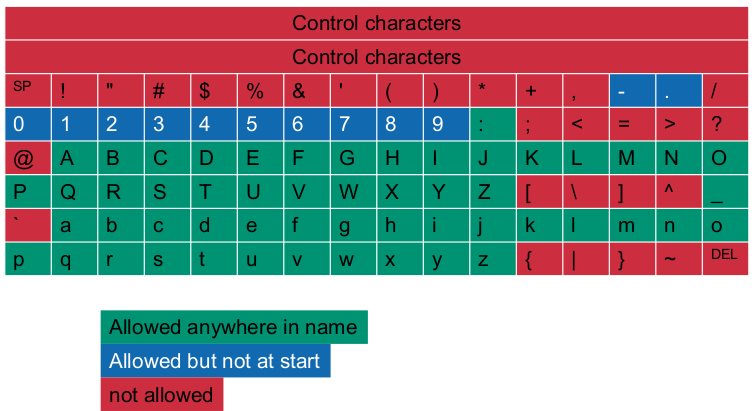
\includegraphics[width=0.5\linewidth]{figures/xml_names}
	\caption{ASCII characters allowed in XML names}
	\label{fig:xmlnames}
\end{figure}

How do you tell well-formedness? An editor (oXygen, ...) will tell you. Note: Indentation does \textit{not} matter in XML - it's only useful to make it more readable.\\

\textbf{CDATA sections:} If you don't want to escape every single $<$ and \& (e.g source code) you can enclose sample of literal code in a CDATA section. A CDATA section is set off by \verb|<![CDATA[ and ]]>|. Everything between the \verb|<![CDATA[ and the ]]>| is treated as raw character data. Less-than signs don’t begin tags. Ampersands don’t start entity references. Everything is simply character data, not markup.

\subsubsection{XML as a data format}

Why Use XML for Data? Before XML, individual programmers had to invent a new data format every time they needed to save a file or send a message. Programmers thus often just used the most convenient format to store data - this made understanding the data format and loading it into any other program extremely difficult. The unique strengths of using XML as a software data format include: simple syntax, support for nesting, easy to debug, language- and platform-independent.

XML can be used in various case:

\begin{compactitem}
	\item Communication protocols: REST APIs, RPC (XML-RPC), SOAP
	\item Object serialization: store the state of persistent objects
	\item File formats: XML as a format to store application data (e.g. game store, spreadsheet, transaction,...)
	\item Databases: XML can play a role in the communications between databases and other software, providing information in an easily reusable form. 
\end{compactitem}

\subsection{YAML - the "Python of JSON"}

\begin{verbatim}
%YAML 1.2
---
Country:
code: 'CH'
name: 'Switzerland'
population: 8014000
currency:
name: 'Swiss Franc'
code: 'CHF'
confederation: true
president : 'Ueli Maurer'
capital: null
cities:
- 'Zurich'
- 'Geneva'
- 'Bern'
description: 'We produce very good chocolate.'
\end{verbatim}

\newpage

\section{Wide column stores}

In the relational model we have a schema that specifies attributes \& types and once this is specified, the table can be filled. Issues with relational databases (RDBMS) are smale scale and the fact that they run on a single machine - PBs of data don't fit!\\
\textbf{Column-Oriented Databases:} Column-oriented databases save their data grouped by columns. The reason to store values on a per-column basis instead is based on the assumption that, for specific queries, not all of the values are needed. HBase is \textbf{not} a column-oriented database in the typical RDBMS sense, but utilizes an on-disk column storage format.


\textbf{Can we fix RDBMs?}
The performance of RDBMSes is well suited for transactional processing, it is less so for very large-scale analytical processing

\begin{compactitem}
	\item Scaling up (more storage etc.) helps a little but doesn't solve the underlying problem $\rightarrow$ we still can't handle PBs of data.
	\item Scaling out (cluster, replicate): People tried this 20 years ago $\rightarrow$ very tedious and it didn't really work. It was further very hard to setup and had high maintenance cost.
\end{compactitem}

Database (De-)Normalization: Design schemas differently - Denormalization, Duplication, and Intelligent Keys (DDI). It is about rethinking how data is stored in Bigtable-like storage systems, and how to make use of it in an appropriate way.

Solution: \textbf{HBase}:

\begin{compactitem}
	\item an open-source tech that allows you to store a relational table on a cluster
	\item By design running on a scalable cluster of commodity hardware
	\item HBase uses HDFS to store data (use a distributed FS to run a DB in a distributed way)
\end{compactitem}

\subsection{Wide column stores: data model}

We first look at the underlying logical model of wide column stores. The founding paper was Google's BigTable. The problem with the tabular model is \textit{expensive joins}. In the tabular model we have lots of tables (BCD normal form) which requires lots of joins $\rightarrow$ very expensive, especially in the distributed setting.\\
As such, the design paradigm of BigTable is: \textit{store together	what is	accessed together} and avoid the whole join complexity (e.g. if customer \& order info is accessed together, put it together). This breaks Boyce-Codd normal form $\rightarrow$ this is bad practice in relational databases. In big data, this is good practice. Keep together what belongs together. This is a shift of paradigm: \textit{denormalize}.

\subsubsection{Logical model of Wide column stores ("key-value model with columns on top")}

The logical model of HBase is \textit{big tables with lots of rows (billions)}. 

\begin{compactitem}
	\item Rows: Each row has a unique identifier (similar to key-value model). The user has full control over the row IDs $\rightarrow$ can specify e.g. country-code at beginning of row ID to group countries together, or use the AHV number. All rows are always sorted lexicographically by their row key.
	\item Columns: HBase has columns (key-value doesn't) and columns are grouped into families. Lots of columns can be in a family (wide-column store... we can have millions of columns per family). Column families must be known in advance and thus can't be pushed too much.
	\item Column families must be known in advance but columns can be added on the fly.
\end{compactitem}

Access to row data is atomic and includes any number of columns being read or written to. There is no further guarantee or transactional feature that spans multiple rows or across tables. The atomic access is also a contributing factor to this architecture being strictly consistent, as each concurrent reader and writer can make safe assumptions about the state of a row.

\subsubsection{Primary queries}

Unlike in the RDBMS landscape, there is no domain-specific language, such as SQL, to query data. Access is not done declaratively, but purely imperatively through the client-side API.

\begin{compactitem}
	\item GET: get row by ID (similar to key-value model)
	\item PUT: put new row with id \& columns into table
	\item SCAN: ask HBase to completely scan the table (typically do something on every row, e.g. comparison) (doesn't exist in KV-model)
	\item DELETE: delete row. When a user deletes a value in an HBase table, this does \textit{not} remove a KeyValue in the MemStore and/or in the HFile where it was stored. HDFS does not support random access. Deleting a value on the logical level creates, on the physical level, a new version of the value flagged as deleted. That way, the next time a query potentially includes this value, it will be omitted from the output by HBase.\\
\end{compactitem}

\textbf{Some terminology:}

\begin{compactitem}
	\item Key-value model: entries are accessed by a key and have some value
	\item Column-oriented storage: instead of storing table row by row, you store the columns (e.g. store all city names in one location)
	\item Wide column stores: millions of columns \& billions of rows $\rightarrow$ quadrillions of cells. This doesn't fit in a single DC?! $\rightarrow$ Wide column stores are typically sparse, thus they fit in a DC.
\end{compactitem}

Examples of wide column stores: Google's BigTable, Apache HBase (open-source), Cassandra.\\

\subsection{HBase: physical level}

Physical layer: How should we split \& distribute over machines? Split table horizontally across machines and split regions vertically across files.
\begin{compactitem}
	\item regions (= continuous set of rows in a range): partition by rows. Rows are sorted by row Id. This allows to specify regions by a range [min-incl.,max-excl.) (open max.). Regions are dynamically split by the system when they become too large.
	\item column families (= column family of one region) are stored together (i.e one file on HDFS)\\
\end{compactitem}

HBase uses the same model as HDFS: master-slave model. Each region is served by exactly one region server, and each of these servers can serve many regions at any time. Splitting and serving regions can be thought of as autosharding, as offered by other systems.

\begin{figure}[hb!]
	\centering
	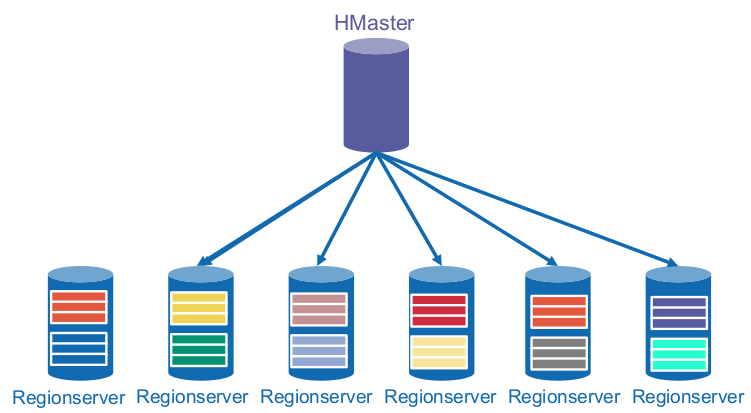
\includegraphics[width=0.4\linewidth]{figures/hbase_master_slave}
	\caption{HBase master-slave model}
	\label{fig:hbasemasterslave}
\end{figure}

\subsubsection{HMaster \& RegionServers}

There are three major components to HBase: the client library, one master server, and many region servers. The region servers can be added or removed while the system is up and running to accommodate changing workloads. The master is responsible for assigning regions to region servers and uses Apache ZooKeeper, a reliable, highly available, persistent and distributed coordination service, to facilitate that task.

\begin{compactitem}
	\item DDL (data definition language) operations: create table, delete table, etc.
	\item \textbf{HMaster} splits table into regions and assigns regions to RegionServers. Someone could keep inserting more \& more rows into a region. Regions must thus be split when they grow too large. HMaster will split large regions into two new regions. The master is not part of the actual data storage or retrieval path.
	\item \textbf{Region servers} are responsible for all read and write requests for all regions they serve, and also split regions that have exceeded the configured region size thresholds. Clients communicate directly with them to handle all data-related operations.
	\item If one RegionServer starts having too many regions, HMaster will rebalance them, i.e. assign region to new RegionServer.
	\item HMaster handles Regionserver failovers. If HMaster sees that a RegionServer failed, he tells another RegionServer that he'll now has to takeover the regions of the failed RegionServer.
	\item Upon a RegionServer failure, we won't loose data! The RegionServers don't actually store data, they are responsible for the regions. The actual data is stored in HDFS. HDFS has replication and is thus failure-resistent. The RegionServer from HDFS perspective is just a client. A single machine runs both a DataNode process and a RegionServer process. The HMaster and NameNode may also run on the same machine.\\
\end{compactitem}

Why do we need HBase when we have HDFS? HBase is there s.t. users don't need to worry about low-level details of HDFS $\rightarrow$ data-independence. Shield users from details of storage.

\subsubsection{Physical storage}

A region is handled by one RegionServer. 

\textbf{Store:} Each region is split into column families. A column family in one region is called a \textbf{Store = (Region, Column family)}. A store is essentially the cartesian product between regions and column families. A store is made of cells. A store is mapped to \textbf{HFiles} on drives. At the beginning (small store) we only have 1 HFile. When the store grows, we'll have multiple HFiles.\\
\textbf{HFile:} We have a mapping of table to files. From the perspective of HDFS, this is just any file. If the HFile gets too large ($>$ 128MB) HDFS splits the HFile into multiple blocks. This doesn't concern HBase. From HBase's view. it's just another file in HDFS $\rightarrow$ modularity.\\
Inside, the HFile works as follows: we essentially break the store into cells and store cells one after another by their key in the HFile. That's actually a sorted list of key-value pairs - keys: row-column(-version) Ids, value: cell-content (e.g cell in row B column 2: key B2).\\
\textbf{Versioning:} We can store multiple old versions of a cell. In GET, we'd just get the latest version. This is used for historical purposes (e.g. price history).\\
\textbf{KeyValue in HBase:} A KeyValue in HBase is the smallest unit of physical storage, indexed by row, column and version, and sharded by regions and column families.

\begin{figure}[hb!]
	\centering
	\begin{subfigure}[t]{.3\textwidth}
		\centering
		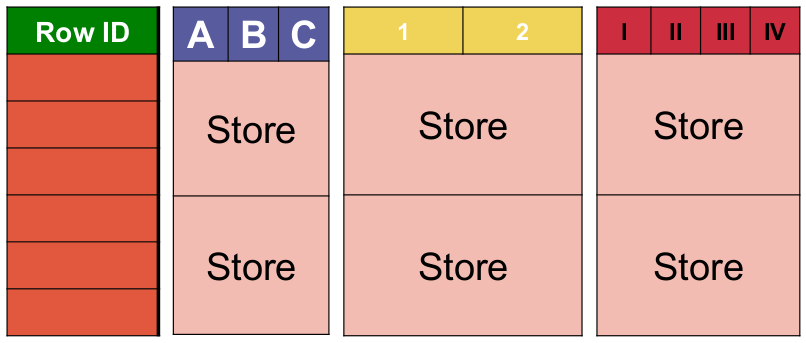
\includegraphics[width=0.9\linewidth]{figures/hbase_physical_storage}
		\caption{Physical storage}
		\label{fig:hbasephysicalstorage}
	\end{subfigure}%
	\begin{subfigure}[t]{.3\textwidth}
		\centering
		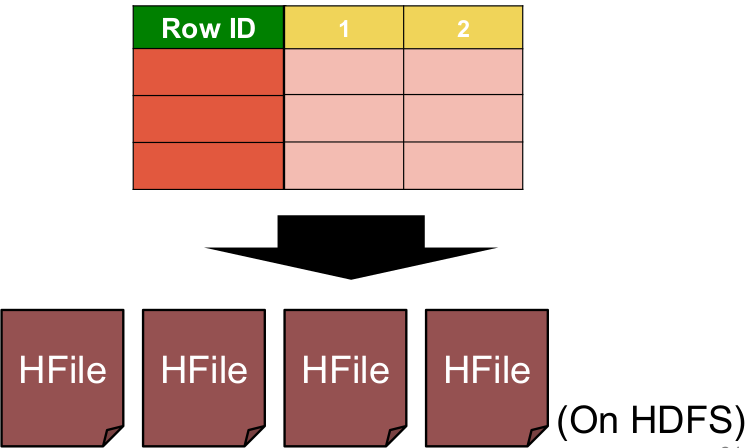
\includegraphics[width=0.9\linewidth]{figures/hbase_store}
		\caption{Store = column family}
		\label{fig:hbasestore}
	\end{subfigure}
	\begin{subfigure}[t]{.3\textwidth}
		\centering
		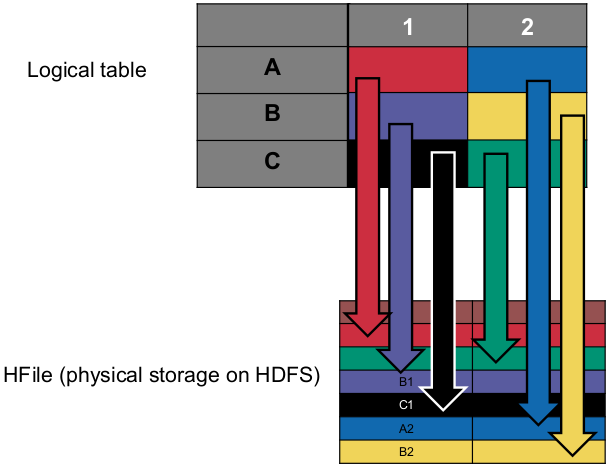
\includegraphics[width=0.9\linewidth]{figures/hbase_hfile}
		\caption{HFile}
		\label{fig:hbasehfile}
	\end{subfigure}
\end{figure}

\begin{figure}[hb!]
	\centering
	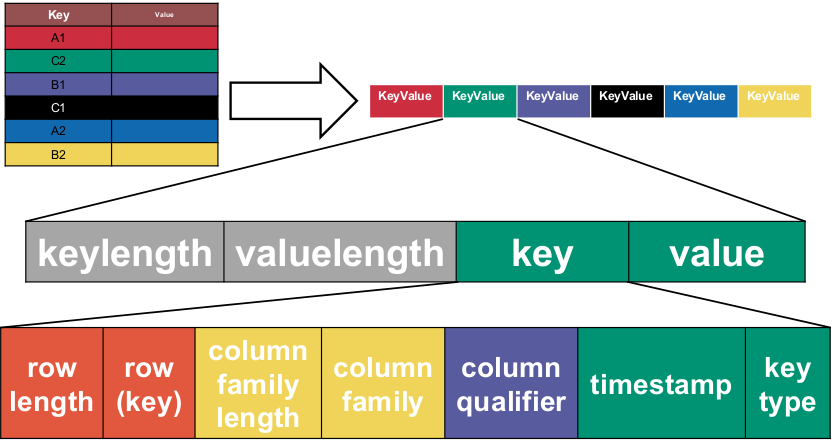
\includegraphics[width=0.35\linewidth]{figures/hfile_key_value}
	\caption{HFile: KeyValue}
	\label{fig:hfilekeyvalue}
\end{figure}

\textbf{HBlocks:} Key-values can be very small (bytes). We don't want to read byte-by-byte in HDFS. But we also don't want to read the whole 128MB block at a time $\rightarrow$ lower grouping of key-values. \textit{HBlocks} are a "Quantity" of KeyValues that get read at a time (default size \textbf{64kb}). Inside the HFile, the key of the first row of the HBlock is used as key to the HBlock. Since keys are sorted, this way we easily find the HBlock in which the wanted key-value pair is located in.

\begin{figure}[hb!]
	\centering
	\begin{subfigure}[t]{.5\textwidth}
		\centering
		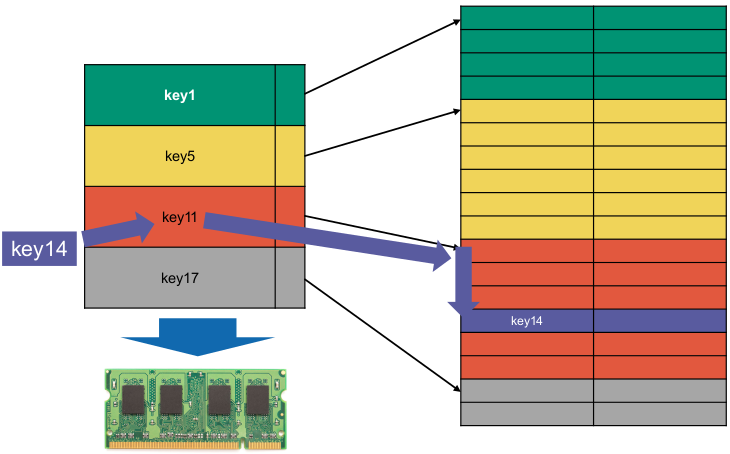
\includegraphics[width=0.9\linewidth]{figures/hbase_hblock_key_lookup}
		\caption{HFile: key lookup in HBlocks}
		\label{fig:hbasehblockkeylookup}
	\end{subfigure}%
	\begin{subfigure}[t]{.5\textwidth}
		\centering
		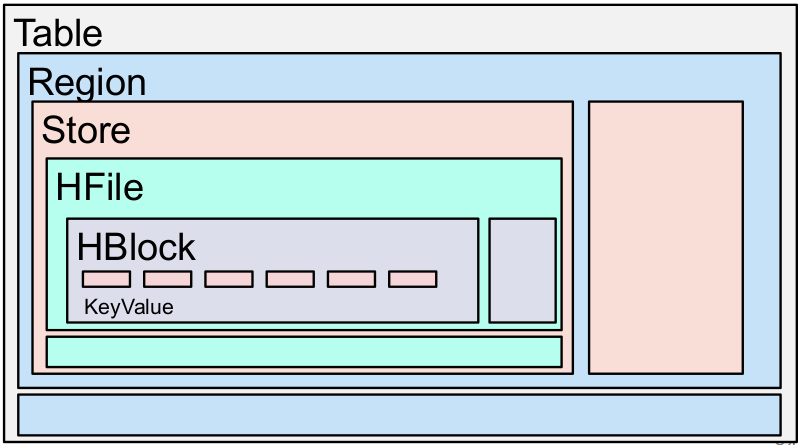
\includegraphics[width=1\linewidth]{figures/hbase_levels_of_phys_storage}
		\caption{Levels of physical storage}
		\label{fig:hbaselevelsofphysstorage}
	\end{subfigure}
\end{figure}

\textbf{Problem:} What about inserting new keys? We can only write key-values in sorted order. We need to maintain the order of keys. \textit{But} in HDFS we can only append, we can't insert in between past lines! Solution: sort the new set of keys, completely flush the old file and create a new file.

\textbf{Writing new cells}\\
We have multiple HFiles, each with multiple HBlocks (filled with key-values) on disk. When a user writes (inserts) a new key-value pair to a HFile, the pair is first stored in memory - not yet in the HFile. At some point the memory is full (when I insert a whole row, a lot of key-value pairs are created - each key-value pair is a cell in the table). Once the memory is full, all the key-values pairs in memory are flushed to HDFS. I.e. all keys from HDFS and memory are sorted and then put into new HFiles.\\
So essentially, instead of writing to HDFS every time we insert a new key-value pair, we aggregate new key-value pairs in memory and then flush simultaneously.

\begin{figure}[hb!]
	\centering
	\begin{subfigure}[t]{.5\textwidth}
		\centering
		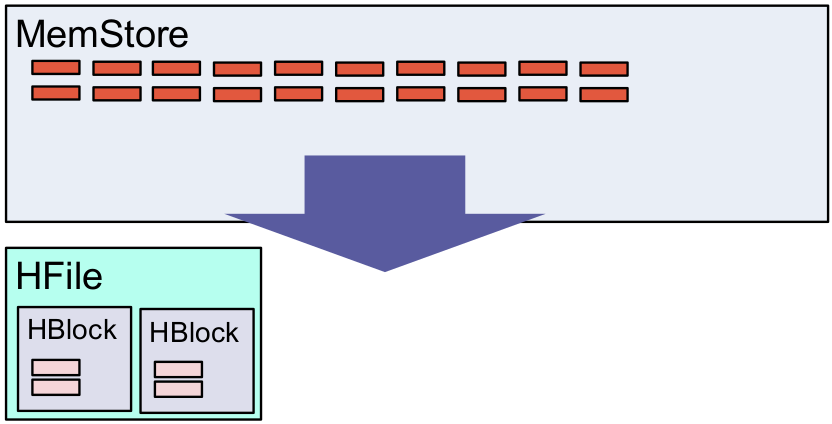
\includegraphics[width=0.7\linewidth]{figures/hbase_write_cells}
		\caption{Writing new cells}
		\label{fig:hbasewritecells}
	\end{subfigure}%
	\begin{subfigure}[t]{.5\textwidth}
		\centering
		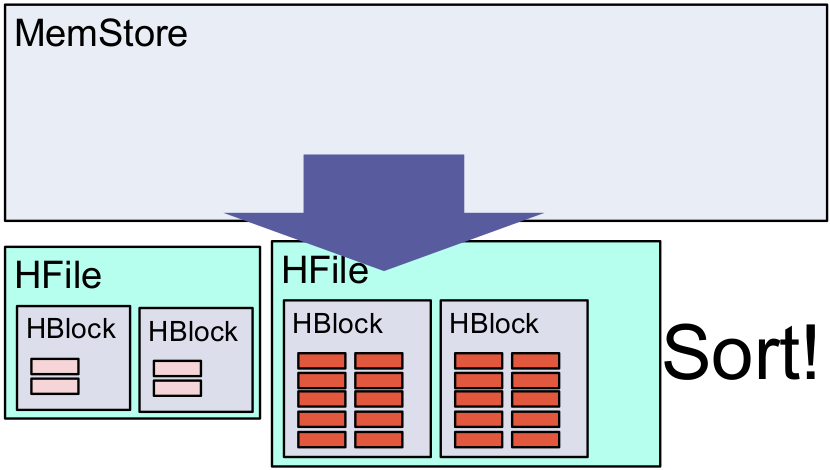
\includegraphics[width=0.7\linewidth]{figures/hbase_flush_cells}
		\caption{Flush cells in memory and sort}
		\label{fig:hbaseflushcells}
	\end{subfigure}
\end{figure}

\textbf{Reading from a Store:}\\
If someone wants to read, we have to look in HFiles \textit{and} in MemStore (since recently added key-value pairs could not have been flushed yet).

\begin{figure}[hb!]
	\centering
	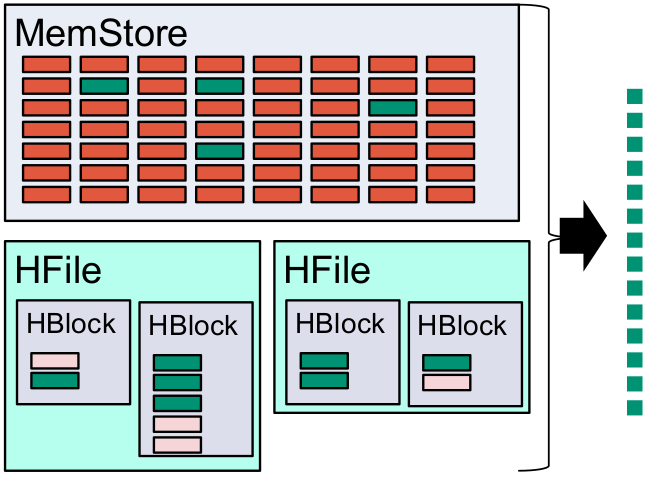
\includegraphics[width=0.3\linewidth]{figures/hbase_read_store}
	\caption{Reading from a Store}
	\label{fig:hbasereadstore}
\end{figure}

\textbf{Compaction:}\\
If we do a lot of flushing, we might end up with lots of HFiles. This is practically bad since in a query we need to look in every single HFile. We can compact them into a single HFile. Compaction uses MergeSort to compact the various HFiles into one HFile. MergeSort is used since it doesn't need to load all data into memory.\\
Seeks vs. transfer: What data structure should we use:

\begin{compactitem}
	\item B+-trees: solve latency issues (store indices on disk). Used by classical RDBMS. Latency-bound.
	\item LSM-Trees: solve throughput issues. Used by wide column stores. Throughput-bound.
\end{compactitem}

\textbf{Log-structured Merge-Trees procedure:} We have lots of cells in memory which causes the memory to be full $\rightarrow$ flush the memory. This creates a new HFile. If we flush over and over, we get many HFiles. Compaction then merges two HFiles into one larger HFile. This is done over and over.

\textbf{HBase Bootstrap: How to start up}\\
If someone wants to start querying, how does he (or the HMaster) know which RegionServer to contact $\rightarrow$ meta table. Meta table stores where regions are stored/ on which RegionServer.\\
Resolution:

\begin{compactenum}
	\item Client contacts HMaster to Create/delete/update table
	\item Client contacts RegionServer that stores the meta table and asks it for a region.
	\item The RegionServer responds with the RegionServer location(s)
	\item Client queries the RegionServer
\end{compactenum}

\subsection{HBase: Underlying APIs}

HBase is implemented in Java and offers a Java and REST API.

\subsection{HBase: caching}

HBase uses HDFS and HDFS can be slow. Thus, HBase will be slow. In order to improve this, HBase uses caching to speed up. The cache contains copies of some cells (according to some caching policy).

When NOT to use the cache:

\begin{compactitem}
	\item Batch processing: If you keep scanning the entire table the cache is useless. Cache is only useful if you access a few hot items.
	\item Random access: If you access random places, the cache will just keep replacing.\\
\end{compactitem}

As a general notion, HBase is fast (even though it runs on top of HDFS, which is slow) because:

\begin{compactitem}
	\item HBase has KeyValues in the MemStore as well as in caches
	\item HBase shortcircuits DataNodes: A RegionServer process is on the same machine as a DataNode process. Thus, the files of a RegionServer are essentially stored 'locally' on disk in HDFS blocks. If the RegionServer knows that the blocks of the HFile it wants to read are directly on the same machine, the RegionServer will \textit{NOT} go through the whole HDFS process of contacting the NameNode, contacting the DataNodes, etc. and instead short circuit that process and directly read the blocks from its local hard drive. This is much faster because you don't have the network overhead.
\end{compactitem}

\subsection{Data Locality}

HBase vs HDFS: How do HDFS and HBase interact with eachother?\\
When you create an HFile, HDFS will create and store it. It will split the HFile into HDFS blocks (128MB). If a RegionServer creates a new HFile, it will communicate with the HDFS NameNode $\rightarrow$ NameNode answers where blocks should be stored in DataNodes. The first replica is placed on the machine where the client is on - the machine that runs the RegionServer (HDFS client) process also runs a DataNode process! Thus at least one replica of each HDFS block that corresponds to an HFile of a RegionServer is stored on the same physical machine as the RegionServer.\\

HDFS may redistribute blocks which could cause some blocks to be on different DataNodes... RegionServer could tell NameNode to put its blocks back on the DataNode that runs on the machine it is running on - but this isn't necessary! \textit{HFile compaction brings back locality} - the new compactified HFile will be located on the DataNode that is on the same machine as the RegionServer.

\subsection{Best practices}

\begin{compactitem}
	\item Number of rows: Millions: RDBMS, Billions: HBase
	\item Number of nodes: HBase needs many nodes to be useful (\textbf{$> 5$}). With just 1 node: use a RDBMS.
	\item Row IDs and column names: Keep them short. Why? Keys are made of row IDs and column names. The keys are stored in every key-value pair $\rightarrow$ long keys use just too much memory.
\end{compactitem}

\subsection{Summary}

HBase is a distributed, persistent, strictly consistent storage system with near-optimal write—in terms of I/O channel saturation—and excellent read performance, and it makes efficient use of disk space by supporting pluggable compression algorithms that can be selected based on the nature of the data in specific column families.\\
There is no declarative query language as part of the core implementation, and it has limited support for transactions. Row atomicity and read-modify-write operations make up for this in practice, as they cover most use cases and remove the wait or deadlock-related pauses experienced with other systems.\\
HBase handles shifting load and failures gracefully and transparently to the clients. Scalability is built in, and clusters can be grown or shrunk while the system is in production. Changing the cluster does not involve any complicated rebalancing or resharding procedure, but is completely automated.

\subsection{HBase shell commands}

\begin{compactitem}
	\item Start shell: hbase shell, Create table: create $<$table$>$, $<$columFamily$>$, $<$columFamily$>$, ...
	\item Check schema: describe $<$table$>$, Count rows: count $<$table$>$
	\item Insert row: put $<$table$>$, $<$rowId$>$, $<$columnFamily:columnQualifier$>$, $<$value$>$
	\item Query row: get $<$table$>$, $<$rowId$>$
	\item Filter by value: scan 'sentences', {FILTER =$>$ "ValueFilter(=, 'binary:English')"}
	\item Column value substring: scan 'sentences', \{COLUMNS =$>$ 'words:subject', FILTER =$>$ "ValueFilter(=, 'substring:I')"\}
	\item Row key prefix: scan 'sentences', \{COLUMNS =$>$ 'words:object', ROWPREFIXFILTER =$>$ 'row'\}
\end{compactitem}

\subsection{Pure row stores vs. pure column stores vs. wide column stores}

\begin{table}[hb!]
\begin{tabular}{|p{15mm}|p{80mm}|p{80mm}|}
	\hline 
	& \textbf{Advantages} & \textbf{Disadvantages} \\ 
	\hline 
	Pure row stores & Good for workloads with point lookups and updates. Retrieving (updating) a single row is efficient as the row is colocated. & Scans are more expensive (whole row is always retrieved). \\ 
	\hline 
	Pure column stores & Scans are very efficient (only specific columns can be retrieved). & To retrieve (or update) a whole row, many random accesses need to be performed. \\ 
	\hline 
	Wide column stores & 
	\begin{compactitem}
		\item Column families offer a 'middle ground' between pure row- and column-oriented storages. Columns frequently accessed together can be colocated, very wide columns (affecting scan speed) can be isolated into separate column families.
		\item Flexible schema (column names stored for each row) offer flexibility for cases where schema is not known upfront (or in cases of sparse columns).
	\end{compactitem}  & 
	\begin{compactitem}
		\item Performance penalties, point lookups not as fast as pure row store, scans not as fast as pure column store.
		\item The key holds the row key, the column family name, the column qualifier, etc. This can result in a considerable storage
		overhead if the values that we want to store are small in comparison the key.
	\end{compactitem}\\
	\hline 
\end{tabular} 
\end{table}

\subsection{Advantages and disadvantages of Denormalization}

\textbf{Advantages:} All operations are either scans or point lookups. No need for expensive joining of multiple relations (all data is colocated or easily mapped).\\

\textbf{Disadvantages:}
\begin{compactitem}
\item It is difficult to enforce (maintain) consistency in cases of updates
\item Storage (memory) overhead, due to duplicated data
\item Scan processing can be more expensive 
\end{compactitem}


\newpage

\section{Data models}

Syntax vs. data model:

\begin{compactitem}
	\item Data model (Logical view): table, tree, etc.
	\item Syntax (Physical view): CSV, JSON, etc.
\end{compactitem}

A syntax (e.g. CSV) is associated with a data model (e.g. table). In RDBMS, we first defined the data model (table) and \textit{then} the syntax (CSV). With XML and JSON, we did the opposite. We first defined the syntax (XML, JSON) and after the tree data model.

\subsection{JSON Data Model}

Two types of values:

\begin{compactitem}
	\item Atomic values: strings, numbers, booleans, null
	\item Structured values: objects (String-to-Value map), arrays (List of values)\\
	$\rightarrow$ both of these offer recursion (i.e. array in array or object in object)
\end{compactitem}

As we know, JSON is a \textbf{tree-based} model:

\begin{figure}[hb!]
	\centering
	\begin{subfigure}[t]{.5\textwidth}
		\centering
		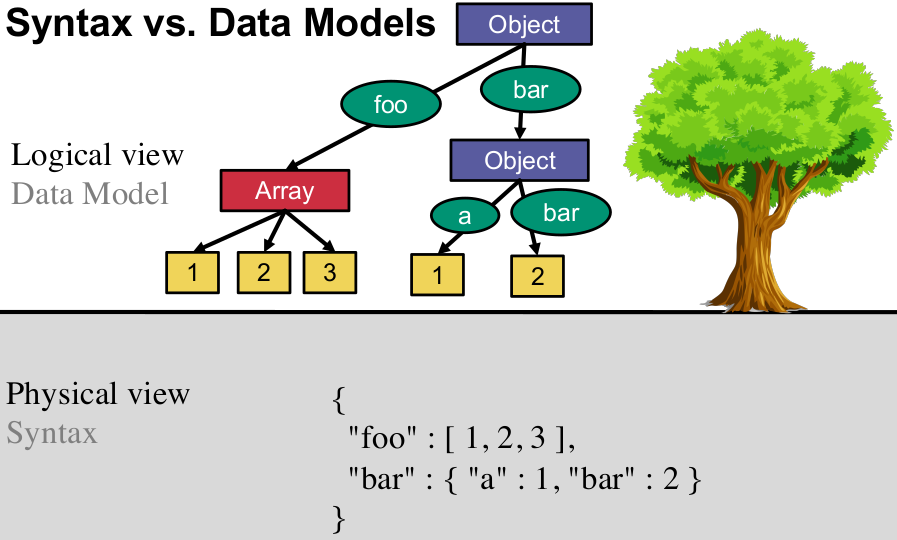
\includegraphics[width=0.9\linewidth]{figures/json_syntax_datamodel}
		\caption{JSON: Syntax vs. Data Models}
		\label{fig:json_syntax_datamodel}
	\end{subfigure}%
	\begin{subfigure}[t]{.5\textwidth}
		\centering
		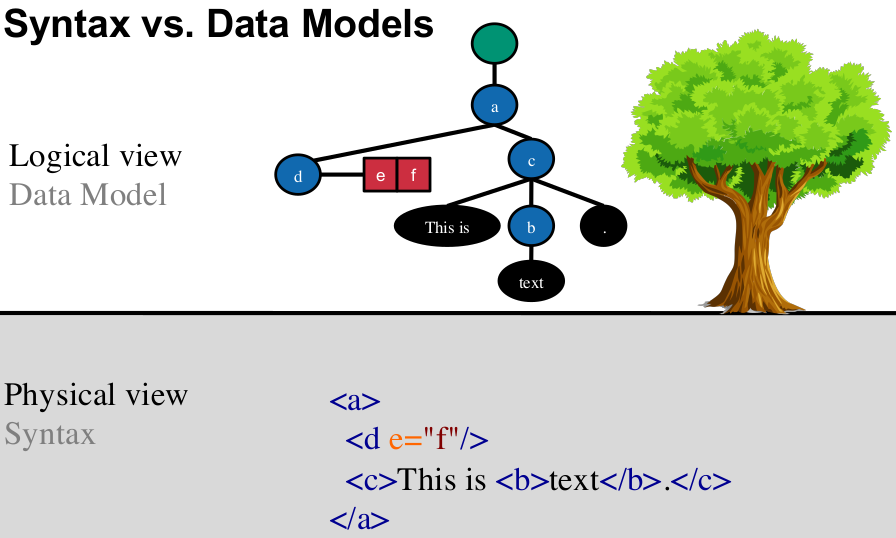
\includegraphics[width=0.9\linewidth]{figures/xml_syntax_datamodel}
		\caption{XML: Syntax vs. Data Models}
		\label{fig:xml_syntax_datamodel}
	\end{subfigure}
\end{figure}

The same holds for XML.\\

The difference between JSON and XML regarding the visual model is that for JSON, the labels are on the edges and for XML, the labels are on the nodes.

\subsection{XML Information Set}

The 11 XML Information Items:

\vspace{-\topsep}
\begin{multicols}{2}
	\begin{compactitem}
		\item \textbf{Document}
		\item \textbf{Element}
		\item \textbf{Attribute}
		\item (Processing Instruction)
		\item \textbf{Character}
		\item (Comment)
		\item (Namespace)
		\item (Unexpanded Entity Reference)
		\item (DTD)
		\item (Unparsed Entity)
		\item (Notation)
	\end{compactitem}
\end{multicols}

\textbf{Example:}
\vspace{-\topsep}
\begin{verbatim}
1: <?xml version="1.0" encoding="UTF-8"?>
2: <!DOCTYPE metadata>
3: <metadata>
4:     <title
5:         language="en"
6:         year="2019"
7:     >Systems Group</title>
8:     <publisher>ETH Zurich</publisher>
9: </metadata>
\end{verbatim}
\vspace{-\topsep}

\textbf{Document Information Items:}

\begin{compactitem}
	\item Document Information Item: doc
	\item \verb|[children]| Element Information Item: metadata
	\item \verb|[version]|: 1.0
\end{compactitem}

\newpage

\textbf{Element Information Items:}
\vspace{-\topsep}
\begin{multicols}{2}
	\begin{compactitem}
		\item Element Information Item: metadata
		\item \verb|[local name]| metadata
		\item \verb|[children]| Element Information Items: title, publisher
		\item \verb|[attributes]| \verb|<empty>|
		\item \verb|[parent]| Document Information Item: doc\\\\
	\end{compactitem}
	
	\begin{compactitem}
		\item Element Information Item: title
		\item \verb|[local name]| title
		\item \verb|[children]| Text Information Items: Systems Group
		\item \verb|[attributes]| Attribute Information Items: language=en, year=2019
		\item \verb|[parent]| Element Information Item: metadata\\
	\end{compactitem}
\end{multicols}

	\begin{compactitem}
	\item Element Information Item: publisher
	\item \verb|[local name]| publisher
	\item \verb|[children]| Text Information Items: ETH Zurich
	\item \verb|[attributes]| Attribute Information Items \verb|<empty>|
	\item \verb|[parent]| Element Information Item: metadata
\end{compactitem}

\textbf{Attribute Information Items:}
\vspace{-\topsep}
\begin{multicols}{2}
	\begin{compactitem}
		\item Attribute Information Item: year=2019
		\item \verb|[local name]| year
		\item \verb|[normalized value]| 2019
		\item \verb|[owner element]| Element Information Item: title
		
		\item Attribute Information Item: language=en
		\item \verb|[local name]| language
		\item \verb|[normalized value]| en
		\item \verb|[owner element]| Element Information Item: title
	\end{compactitem}
\end{multicols}
\vspace{-\topsep}

\textbf{Text Information Items:}
\vspace{-\topsep}
\begin{multicols}{2}
	\begin{compactitem}
		\item Text Information Item: Systems Group
		\item \verb|[characters]| S y s t e m s \verb|<space>| G r o u p
		\item \verb|[owner element]| Element Information Item: title
		
		\item Text Information Item: ETH Zurich
		\item \verb|[characters]| E T H \verb|<space>| Z u r i c h
		\item \verb|[owner element]| Element Information Item: publisher
	\end{compactitem}
\end{multicols}
\vspace{-\topsep}

\begin{figure}[hb!]
	\centering
	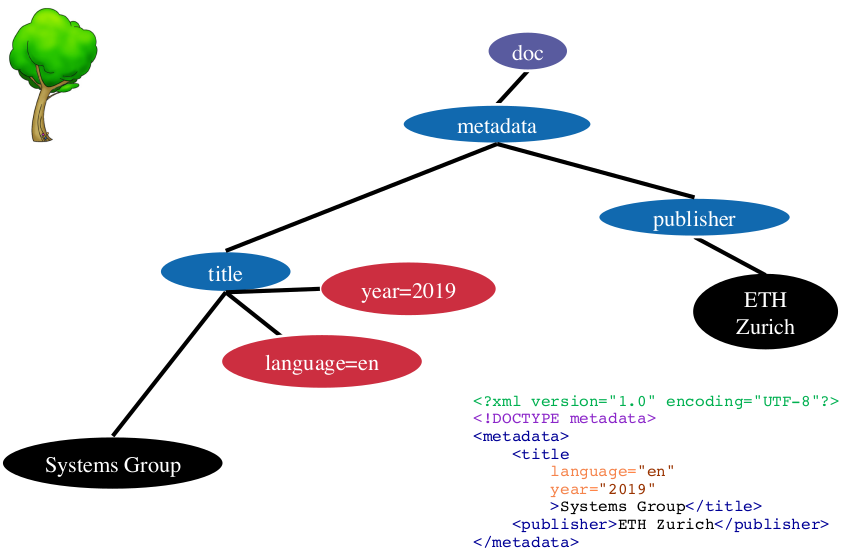
\includegraphics[width=0.39\linewidth]{figures/xml_infoset_tree}
	\caption{XML Infoset - the tree}
	\label{fig:xmlinfosettree}
\end{figure}

\subsection{Types}

\textbf{Type systems:} Almost all type systems (Java, SQL, PSVI, JDM, Protocol buffers, Avro, Parquet, and so on) share the following properties:

\begin{compactitem}
	\item Distinction between \textbf{atomic} types and \textbf{structured} types
	\item \textbf{Same categories} of atomic types
	\item \textbf{Lists} and \textbf{maps} as structured types
	\item Sequence type \textbf{cardinalities}
\end{compactitem}

Types (general): \textit{Atomic types vs. structured types}

\subsubsection{Atomic types}

\textbf{Strings:} Character sequences with monoid structure

\textbf{Numbers:}
\begin{compactitem}
	\item Interval-based integer types: exist as signed and unsigned, different lengths (16-bit, 32-bit, etc.)
	\item Arbitrary precision decimals (and integers): this needs some library (e.g. in Java big int, big float). These offer any precision and any scale (can have 1000s of digits after comma)\\
	$\rightarrow$ in XML \& JSON, this works! There is no size limit on numbers, just put all digits
	\item Float and Double	(IEEE 754 standard)
	\begin{compactitem}
		\item single precision: 32bit, ca. 7 digits, $10^{-37}$ to $10^{37}$
		\item double precision: 64bit, ca. 15 digits, $10^{-307}$ to $10^{308}$
	\end{compactitem}	
\end{compactitem}

\textbf{Booleans:} true, false (different names exist: t/f, y/n, on/off, etc.)\\
\textbf{Dates and Times:} (quite important but overlooked):
\begin{compactitem}
	\item date (a certain day, Gregorian calendar): Year + Month + Day, e.g. 2020-March-30
	\item time: Hours + Minutes + Seconds, e.g. 10:31:15.109378
	\item timestamp (date+time): Year + Month + Day + Hours + Minutes + Seconds,\\
	e.g. 2020-March-30 10:31:15.109378
\end{compactitem}
$\rightarrow$ date and time are \textit{still} not completely standardized\\

\textbf{Time Intervals:} Two duration kinds
\begin{compactitem}
	\item years + months, e.g. 2 years and 4 months
	\item hours + minutes + ..., e.g. 3 hours and 14 minutes
\end{compactitem}
$\rightarrow$ \textit{never} mix months and days in duration, because a month can be 28,29,30,31 days!\\
\textbf{Binaries:} just a bunch of 0s and 1s\\
\textbf{Null:} exists in many schemas, languages, etc.\\

\textbf{Lexical space vs. value space:}

\begin{compactitem}
	\item Value space: the mathematical value (concept of value), e.g. the number 10
	\item Lexical space: the representation in syntax of the value, e.g. $10_{dec}, 1010_{bin}, A_{hex},+10E00_{sci}...$\\
\end{compactitem}

\textbf{Subtypes:}

This is a similar concept to classes and subclasses in OO languages. Example of subtypes: integer is a subtype of decimal. Abstract perspective: value spaces. A type's value space is all values a type can have. A subtype means that the value space of the subtype is a subset of the supertype's value space.

\subsubsection{Structured Types}

Structured types are almost always the same: \textit{Maps (Key-value model!) \& Lists}

\begin{tabular}{|c|c|}
	\hline 
	\textbf{Data Structure} & \textbf{Examples} \\ 
	\hline 
	Maps (Key-value model!)& JSON Object, Set of XML Attributes, Protobuf Message \\ 
	\hline 
	Lists & JSON Array,	XML Element, Protobuf repeated field \\ 
	\hline 
\end{tabular} 

\hfill

\textbf{Cardinality:} not available in all languages

\begin{tabular}{|c|c|c|}
	\hline 
	\textbf{How many?} & \textbf{Common sign} & \textbf{Common adjective} \\ 
	\hline 
	One &  & required \\ 
	\hline 
	Zero or more & * & repeated \\ 
	\hline 
	Zero or one & ? & optional \\ 
	\hline 
	One or more & + &  \\ 
	\hline 
\end{tabular}

\hfill

\subsection{Protocol Buffers}

In the 70s, the 'typical' way to define something was to first define a class that defines an object. Then, you instantiate the class as an object. This is the way it's done in RDBMS and in most programming languages - and this is also how it's done in Protobuf.

Protobuf is language neutral and will convert messages to different languages. This allows to share data between different languages. A Protobuf message defines a \textbf{schema}:
\vspace{-\topsep}
\begin{verbatim}
message Person {
  required string last_name = 1;
  repeated string first_name = 2;
  optional Title title = 3;
  optional Person boss = 4;
}
\end{verbatim}
\vspace{-\topsep}

\textbf{Scalar types:}
\vspace{-\topsep}
\begin{multicols}{2}
	\begin{compactitem}
		\item double, float
		\item int32, int64 and variants
		\item bool
		\item string
		\item bytes
	\end{compactitem}
\end{multicols}

\newpage

\textbf{Enums:} enumeration
\vspace{-\topsep}
\begin{verbatim}
enum Title {
  MR = 1;
  MS = 2;
  MRS = 3;
}
\end{verbatim}
\vspace{-\topsep}

\hfill

e.g. in C++: \verb|person.boss().first_name()|

This is essentially a 'query' for the firstname of the boss person. Protobuf builds methods, functions etc. in a specified language (e.g. C++) $\rightarrow$ one can then access this.

\textbf{JSON/XML vs. Protobufs:}

\begin{compactitem}
	\item With schema (homogeneous, e.g. Protobuf): always the same schema - RDBMS has this - always the same fields and types must match.
	\item No schema	(heterogeneous, e.g. JSON, XML): This is the new thing - get rid of schema! We just have a syntax (JSON, XML) but don't specify a schema. The objects in the syntax can vary \textit{widely}. \textbf{But}: schemas are still useful. We just worry about the schema later. First, create the data, then compare it to a schema.
\end{compactitem}

Not having a schema can be very powerful, e.g. when we just want to dump data. But without a schema, things can get messy. One can also enforce schemas on a heterogeneous syntax! You can introduce a schema to make objects look a certain way. A syntax should then be well-formed \textit{AND} should fulfill some additional properties (schema). E.g. in JSON doc, all values for key "b" are boolean.\\


\subsection{Validation}

Many applications need a more powerful and expressive validation method.

\begin{figure}[hb!]
	\centering
	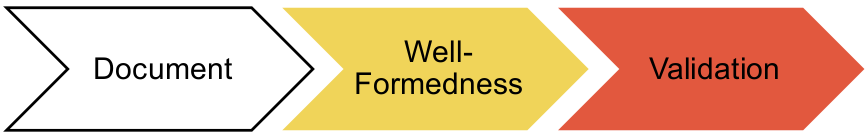
\includegraphics[width=0.4\linewidth]{figures/validation_pipeline}
	\label{fig:validationpipeline}
\end{figure}

\begin{compactitem}
	\item Document: just text
	\item Well-formedness: is text well-formed, i.e. valid syntax (well-formed JSON, XML,...)
	\item Validation: is text valid against a particular \textit{schema} $\rightarrow$ \textit{validation always needs a schema}. There is no absolute notion of validity.
\end{compactitem}

\begin{center}
	valid XML $\neq$ well-formed XML
\end{center}
\vspace{-\topsep}

Validation can only be checked on a well-formed document! We thus have to first check well-formedness and then validity. A well-formed document can be valid against schema A and invalid against schema B.

\textbf{Validation vs. Annotation:}

\begin{compactitem}
	\item Validation: check text against schema. Validity can only be checked on a well-formed document.
	\item Annotation: in XML, we only have text, no int, bool, etc. We can 'stamp' text in XML as int, bool, etc.	
\end{compactitem}


\subsection{XML Schema}

An XML Schema is an XML document containing a formal description of what comprises a valid XML document. An XML document described by a schema is called an instance document.

The following is well-formed XML. We can define a schema on this XML document such that element \verb|foo| has type string (or int,...).

\begin{multicols}{2}
\lstset{language=XML}
\begin{lstlisting}
<?xml version="1.0" encoding="UTF-8"?>
<xs:schema
xmlns:xs="http://www.w3.org/2001/XMLSchema">
  <xs:element name="foo" type="xs:string"/>
</xs:schema>
\end{lstlisting}
	
\lstset{language=XML}
\begin{lstlisting}
<?xml version="1.0" encoding="UTF-8"?>
<foo>
  This is text.
</foo>
\end{lstlisting}
\end{multicols}

\begin{multicols}{2}
\lstset{language=XML}
\begin{lstlisting}
<?xml version="1.0" encoding="UTF-8"?>
<xs:schema
xmlns:xs="http://www.w3.org/2001/XMLSchema">
  <xs:element name="foo" type="xs:integer"/>
</xs:schema>
\end{lstlisting}
	
\lstset{language=XML}
\begin{lstlisting}
<?xml version="1.0" encoding="UTF-8"?>
<foo>
  142857
</foo>
\end{lstlisting}
\end{multicols}

\subsubsection{Simple Types}

A simple element is an XML element that contains only text. It cannot contain any other elements or attributes.

Built-in:

\begin{tabular}{|l|p{150mm}|}
	\hline 
	Strings & string, anyURI, QName \\ 
	\hline 
	Numbers & decimal, integer, float, double, long int, short byte, positiveInteger, \newline nonNegativeInteger..., unsignedLong unsignedInt... \\ 
	\hline 
	Booleans & boolean \\ 
	\hline 
	Dates and Times & dateTime, time, date, gYearMonth, gMonthDay, gYear, gMonth, gDay, dateTimeStamp \\ 
	\hline 
	Time Intervals & duration, yearMonthDuration, dayTimeDuration \\ 
	\hline 
	Binaries & hexBinary base64Binary \\ 
	\hline 
	Null & - \\ 
	\hline 
\end{tabular} 

\subsubsection{User-defined types}

\begin{compactitem}
	\item Restriction, e.g. string of char length 3
	\item Union (not atomic), e.g. integers or booleans
	\item List (not atomic), e.g. list of strings
\end{compactitem}

\subsubsection{Complex types}

A complex element contains other elements and/or attributes. There are four kinds of complex elements: empty elements, elements that contain only other elements, elements that contain only text, elements that contain both other elements and text. Each of these elements may contain attributes as well!


\begin{compactitem}
	\item Empty, e.g. \verb|<product pid="1345"/> |
	\item Simple content, e.g. \verb|<foo>text</foo>|
	\item Complex Content, e.g.
	\begin{verbatim}
		<foo><a/><b/></foo>
	\end{verbatim}
	\item Mixed Content: character data can appear along elements in body of associated element, e.g.
	\begin{verbatim}
		<foo>
		  Text<a/>Text<b/>
		</foo>
	\end{verbatim}
\end{compactitem}

\subsection{XML schemas: some examples}

\lstset{language=XML}
\begin{lstlisting}
<?xml version="1.0"?>
<xs:schema xmlns:xs="http://www.w3.org/2001/XMLSchema"
targetNamespace="https://www.w3schools.com"
xmlns="https://www.w3schools.com"
elementFormDefault="qualified">

<xs:element name="note">
 <xs:complexType>
  <xs:sequence>
   <xs:element name="to" type="xs:string"/>
   <xs:element name="from" type="xs:string"/>
   <xs:element name="heading" type="xs:string"/>
   <xs:element name="body" type="xs:string"/>
  </xs:sequence>
 </xs:complexType>
</xs:element>

</xs:schema> 
\end{lstlisting}

A corresponding XML document that references the schema:

\lstset{language=XML}
\begin{lstlisting}
<?xml version="1.0"?>
<note xmlns="https://www.w3schools.com"
xmlns:xsi="http://www.w3.org/2001/XMLSchema-instance"
xsi:schemaLocation="https://www.w3schools.com note.xsd">

<note>
 <to>Tove</to>
 <from>Jani</from>
 <heading>Reminder</heading>
 <body>Don't forget me this weekend!</body>
</note> 
\end{lstlisting}

\textbf{Simple element}:

\lstset{language=XML}
\begin{lstlisting}
<xs:element name="lastname" type="xs:string"/>
<xs:element name="age" type="xs:integer"/>
<xs:element name="dateborn" type="xs:date"/>
<xs:element name="color" type="xs:string" default="red"/> 
<xs:element name="color" type="xs:string" fixed="red"/> 
\end{lstlisting}

Simple elements can have a default OR a fixed value specified.\\

\textbf{Attributes}: Simple elements cannot have attributes. If an element has attributes, it is considered to be of a complex type. But the attribute itself is always declared as a simple type.

\lstset{language=XML}
\begin{lstlisting}
<xs:attribute name="xxx" type="yyy"/> 
<xs:attribute name="lang" type="xs:string" default="EN"/> 
<xs:attribute name="lang" type="xs:string" fixed="EN"/> 
<xs:attribute name="lang" type="xs:string" use="required"/> 
\end{lstlisting}
Attributes may have a default value OR a fixed value specified. A default value is automatically assigned to the attribute when no other value is specified. Attributes are optional by default. To specify that the attribute is required, use the "use" attribute.\\

\textbf{Restrictions:} Restrictions are used to define acceptable values for XML elements or attributes. Restrictions on XML elements are called facets.

The example below defines an element called "car" with a restriction. The only acceptable values are: Audi, BMW:
\lstset{language=XML}
\begin{lstlisting}
<xs:element name="car">
 <xs:simpleType>
  <xs:restriction base="xs:string">
   <xs:enumeration value="Audi"/>
   <xs:enumeration value="BMW"/>
  </xs:restriction>
 </xs:simpleType>
</xs:element>
\end{lstlisting}

The example below defines an element called "letter" with a restriction. The only acceptable value is ONE of the LOWERCASE letters from a to z:
\lstset{language=XML}
\begin{lstlisting}
<xs:element name="letter">
 <xs:simpleType>
  <xs:restriction base="xs:string">
   <xs:pattern value="[a-z]"/>
  </xs:restriction>
 </xs:simpleType>
</xs:element>
\end{lstlisting}

The next example defines an element called "choice" with a restriction. The only acceptable value is ONE of the following letters: x, y, OR z:
\lstset{language=XML}
\begin{lstlisting}
<xs:element name="choice">
 <xs:simpleType>
  <xs:restriction base="xs:string">
   <xs:pattern value="[xyz]"/>
  </xs:restriction>
 </xs:simpleType>
</xs:element> 
\end{lstlisting}

\newpage

The next example defines an element called "gender" with a restriction. The only acceptable value is male OR female:
\lstset{language=XML}
\begin{lstlisting}
<xs:element name="gender">
 <xs:simpleType>
  <xs:restriction base="xs:string">
   <xs:pattern value="male|female"/>
  </xs:restriction>
 </xs:simpleType>
</xs:element> 
\end{lstlisting}

This example defines another element called "password" with a restriction. The value must be minimum five characters and maximum eight characters:
\lstset{language=XML}
\begin{lstlisting}
<xs:element name="password">
 <xs:simpleType>
  <xs:restriction base="xs:string">
   <xs:minLength value="5"/>
   <xs:maxLength value="8"/>
  </xs:restriction>
 </xs:simpleType>
</xs:element> 
\end{lstlisting}

\textbf{Complex elements:}

Complex element \textit{employee} with simple elements \textit{firstname, lastname} as children.
\lstset{language=XML}
\begin{lstlisting}
<xs:element name="employee">
 <xs:complexType>
  <xs:sequence>
   <xs:element name="firstname" type="xs:string"/>
   <xs:element name="lastname" type="xs:string"/>
  </xs:sequence>
 </xs:complexType>
</xs:element> 
\end{lstlisting}

Complex Empty Element \verb|<product prodid="1345" />|:
\lstset{language=XML}
\begin{lstlisting}
<xs:element name="product">
 <xs:complexType>
  <xs:complexContent>
   <xs:restriction base="xs:integer">
    <xs:attribute name="prodid" type="xs:positiveInteger"/>
   </xs:restriction>
  </xs:complexContent>
 </xs:complexType>
</xs:element> 
\end{lstlisting}

Complex simple content: The following example declares a complexType, "shoesize". The content is defined as an integer value, and the "shoesize" element also contains an attribute named "country":
\lstset{language=XML}
\begin{lstlisting}
<xs:element name="shoesize">
 <xs:complexType>
  <xs:simpleContent>
   <xs:extension base="xs:integer">
    <xs:attribute name="country" type="xs:string" />
   </xs:extension>
  </xs:simpleContent>
 </xs:complexType>
</xs:element> 
\end{lstlisting}

\newpage

\textbf{Order Indicators:} Order indicators are used to define the order of the elements.
\begin{compactitem}
\item The $<$all$>$ indicator specifies that the child elements can appear in any order, and that each child element must occur only once.
\item The $<$choice$>$ indicator specifies that either one child element or another can occur.
\item The $<$sequence$>$ indicator specifies that the child elements must appear in a specific order.
\end{compactitem}

\textbf{Occurrence Indicators:} Occurrence indicators are used to define how often an element can occur.
\begin{compactitem}
\item The $<$maxOccurs$>$ indicator specifies the maximum number of times an element can occur.
\item The $<$minOccurs$>$ indicator specifies the minimum number of times an element can occur.
\item The $<$sequence$>$ indicator specifies that the child elements must appear in a specific order.
\end{compactitem}

\subsection{JSON schema example}

\begin{lstlisting}[basicstyle=\footnotesize]
schema={
 'type': 'object',
 'properties': {
  'target': {'type': 'string'},
  'choices': {'type': 'array', 'items': {'type': 'string'}},
  'guess': {'type': 'string'},
  'date': {'type': 'string'},
  'country': {'type': 'string'},
  'sample': {'type': 'string'}
 },
'required': ['target', 'choices', 'date', 'country', 'sample']}
\end{lstlisting}



\newpage

\section{Distributed Computations I: MapReduce}

\textbf{Basic idea of MapReduce at an example:} count pokemons. Map phase: Distribute sets of Pokemons to many people. Each person counts how many of each Pokemon type he has (i.e. map some part of the input to some intermediate representation). Phase 2: Each person is responsible for counting a set of specific Pokemon types. Each person asks all other for their counts of the Pokemons they are responsible for and then adds all these counts up (i.e. reduce the intermediate representation).\\

MapReduce is the processing stage - needs data. Our data can be in HDFS, HBase, S3, etc. and can have various shapes (text, tables (CSV), trees (XML, JSON), binary files, etc.). The common scenario is HDFS with data split over many HDFS files. The data is only useful for MapReduce if we can query it in parallel - data is spread over many machines and many CPUs $\rightarrow$ since storage is already distributed, we also want queries to be in parallel.

\subsection{MapReduce}

In data processing, the input data is typically sharded (comes in chunks), therefore the output is typically sharded as well. In the ideal case each output shard depends on one single input shard, this allows every machine to just work on its own data; however, this rarely happens in real life. The worst case is when every output chunk depends on every input chunk; this needs lots of communication, which is slow. The typical case is a mix of the two.

\begin{figure}[hb!]
	\centering
	\begin{subfigure}[t]{.3\textwidth}
		\centering
		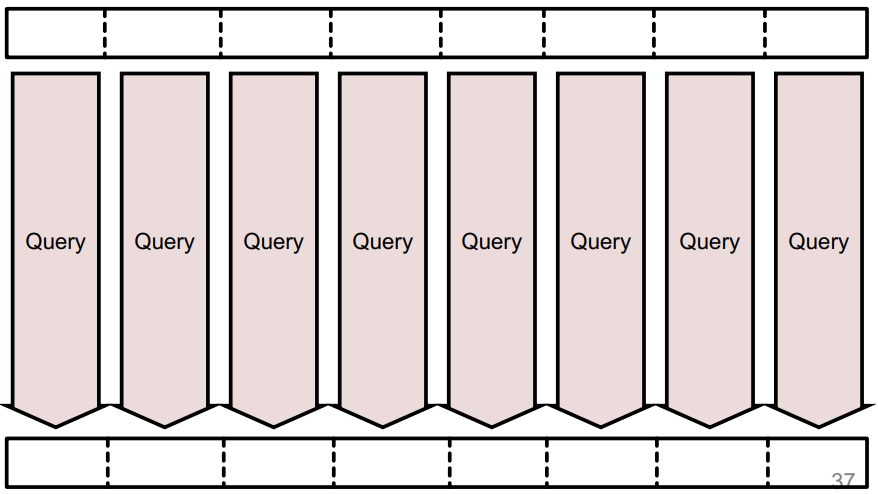
\includegraphics[width=0.9\linewidth]{figures/mr_ideal}
		\caption{Ideal case}
		\label{fig:mrideal}
	\end{subfigure}%
	\begin{subfigure}[t]{.3\textwidth}
		\centering
		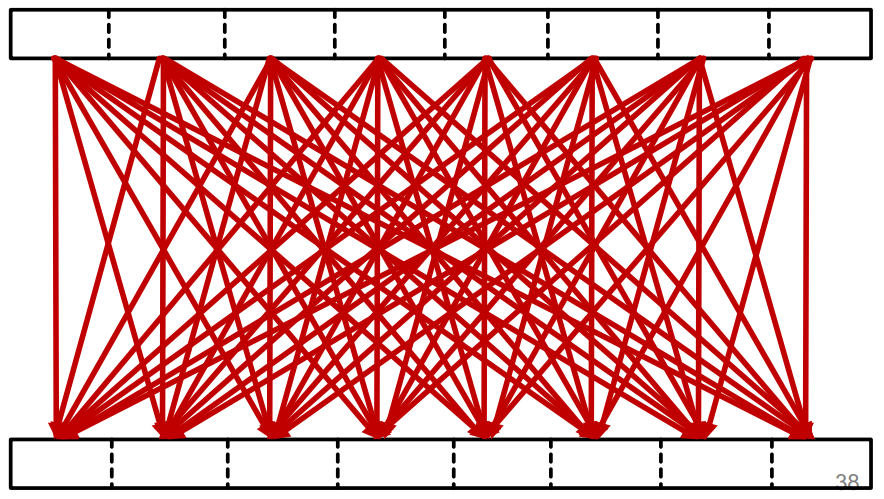
\includegraphics[width=0.9\linewidth]{figures/mr_worst}
		\caption{Worst case}
		\label{fig:mrworst}
	\end{subfigure}
	\begin{subfigure}[t]{.3\textwidth}
		\centering
		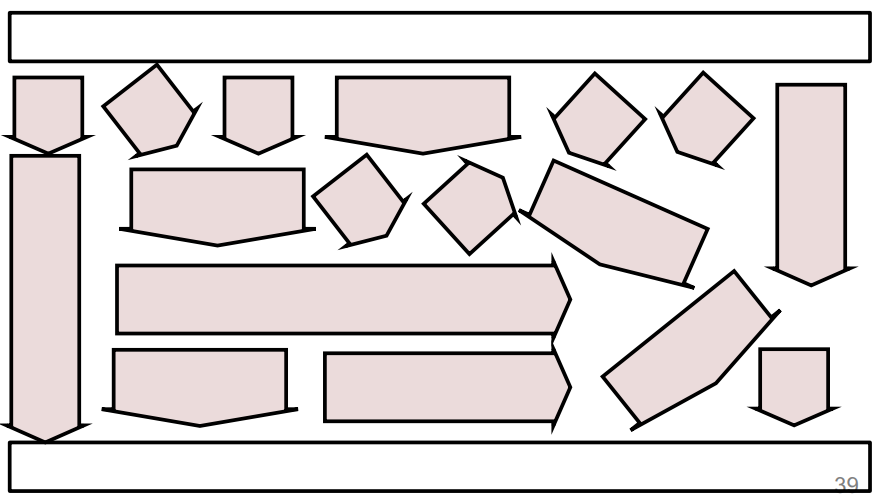
\includegraphics[width=0.9\linewidth]{figures/mr_typical}
		\caption{Typical case}
		\label{fig:mrtypical}
	\end{subfigure}
	\caption{Data processing cases}
\end{figure}

\begin{figure}[hb!]
	\centering
	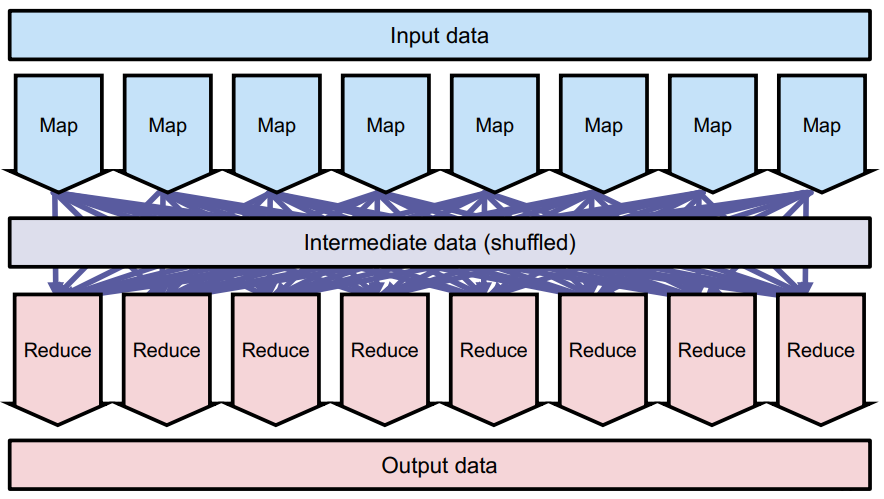
\includegraphics[width=0.5\linewidth]{figures/mr_datamodel}
	\caption{Data Processing: Data Model}
	\label{fig:mrdatamodel}
\end{figure}


The idea of MapReduce is to do the ideal and worst case (mapping and shuffling) in an ordered way.\\

\subsubsection{Logical walkthrough}

\begin{compactenum}
	\item \textbf{Splitting:} The key-value input (converted from some data input) is split into logical chunks.
	\item \textbf{Mapping:} Associate one key-value to one or more key-values through some mapping function. Every key is mapped in parallel. We have splits $\rightarrow$ within each split, I call mapping on each key-value in the split and this is done in parallel for all splits.
	\item \textbf{Put it together:} Put all intermediate key-values together and sort them by key. Then repartition the keys \textit{but} make sure that all key-values with the same key are in the same partition! We can have several key-values in one partition but not one key-value in several partitions.
	\item \textbf{Reduce:} Take intermediate partitions and produce the output by applying the reduce function to the IR key-values in parallel. The output of one key-value set can be one or more key-values (typically just one).
\end{compactenum}

\begin{figure}[t!]
	\centering
	\begin{subfigure}[t]{.3\textwidth}
		\centering
		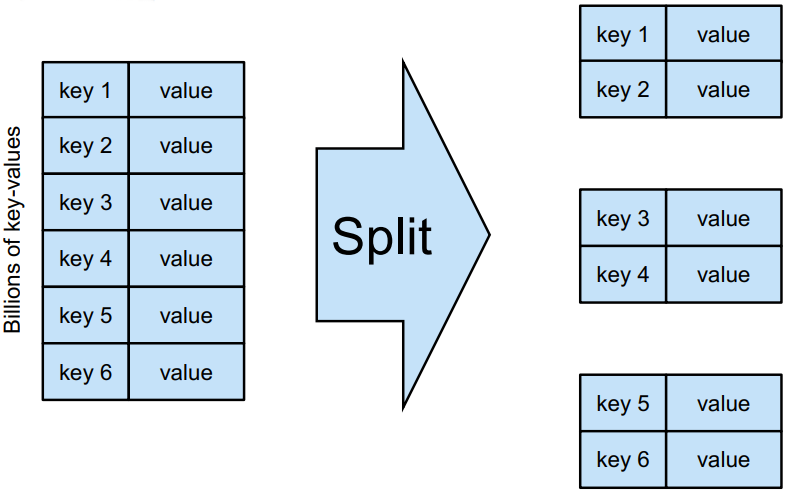
\includegraphics[width=0.9\linewidth]{figures/mr_splitting}
		\caption{Splitting}
		\label{fig:mrsplitting}
	\end{subfigure}%
	\begin{subfigure}[t]{.3\textwidth}
		\centering
		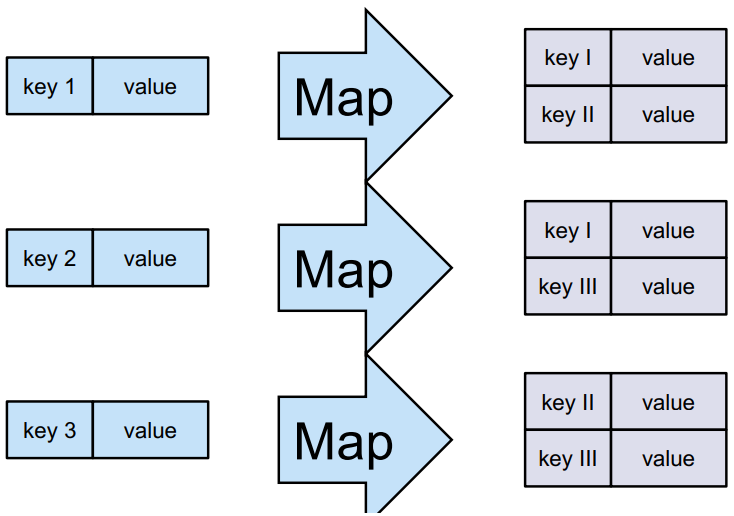
\includegraphics[width=0.9\linewidth]{figures/mr_mapping}
		\caption{Mapping}
		\label{fig:mrmapping}
	\end{subfigure}
	\begin{subfigure}[t]{.3\textwidth}
		\centering
		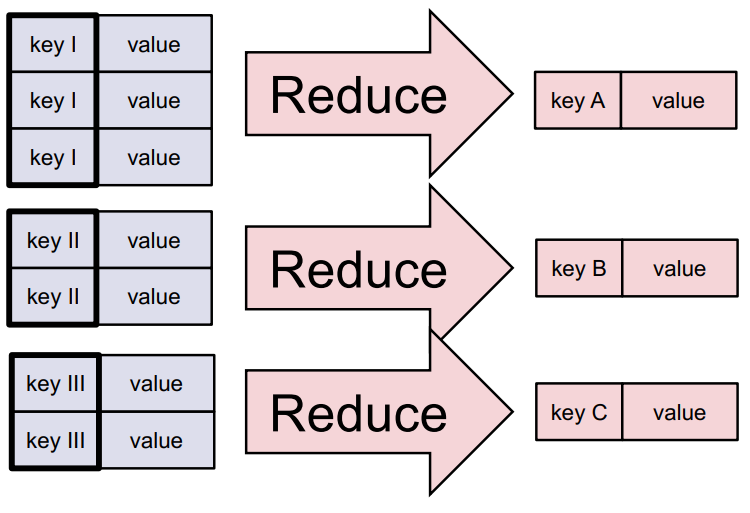
\includegraphics[width=0.9\linewidth]{figures/mr_reduce}
		\caption{Reduce}
		\label{fig:mrreduce}
	\end{subfigure}
	\caption{MapReduce stages}
\end{figure}

\begin{figure}[t!]
	\centering
	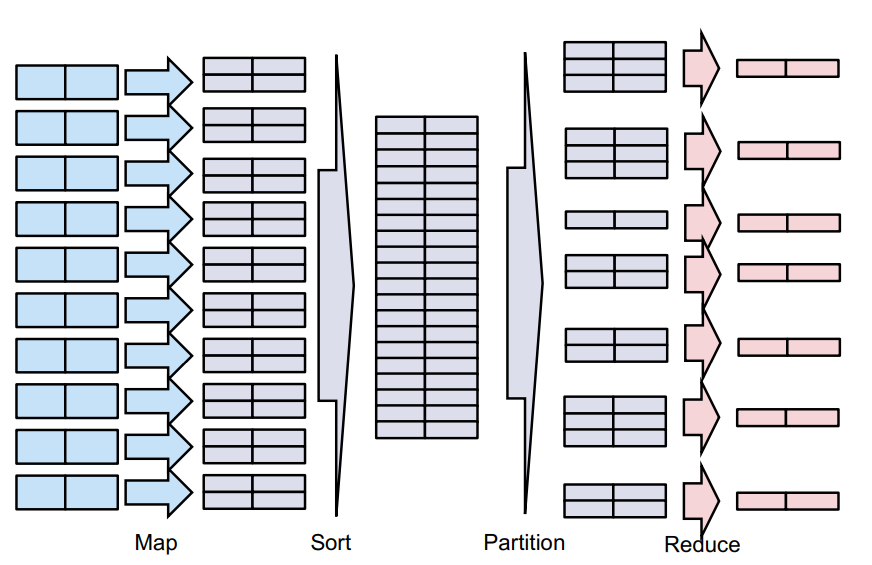
\includegraphics[width=0.4\linewidth]{figures/mr_overall}
	\caption{MapReduce overall}
	\label{fig:mroverall}
\end{figure}

\subsection{Architecture}

MapReduce can run on different storage layers: Local file system, HDFS (most common), S3, Azure Blob storage,... Numbers: we have several TBs of data and 1000s of nodes. What kind of architecture do we have?\\

\textbf{Mater-slave architecture} (again): Just like in HDFS and HBase, we also have a Master-slave architecture for MapReduce. If we use HDFS, HDFS runs on the same machines as MapReduce!
\begin{compactitem}
\item JobTracker (Master): The JobTracker assigns map and reduce tasks, tells respective keys to reducers, etc. The JobTracker typically runs on the same machine as the NameNode in HDFS.

\item TaskTracker (Slave): A TaskTracker runs on each one of the nodes that run DataNodes, and spawns 0,1, or more mappers as well as 0,1, or more reducers according to pre-allocated map and reduce slots. Mappers mostly read their input locally. When all mappers have completed their tasks, the reducers start requesting the intermediate output relevant to them (shuffle). When the reducers have completed, they mostly write their output locally. The TaskTracker typically runs on the same machine as a DataNode.
\end{compactitem}

Running the TaskTracker on the same machine as the DataNode allows the TaskTracker to work with \textit{local data} $\rightarrow$ \textbf{short-circuiting, bring the query to the data}. We don't need to bring the blocks anywhere, bring the query to the data and execute on the machine where the blocks are.\\

\textbf{Mapping phase:} In MapReduce, the input data is \textit{split} (= shard/chunk of the input data). Generally, we have one split per block (128MB) and we only look at one replica per block. The number of mappers is equal to the number of splits. The JobTracker's task is to tell the machines which mappings to do where $\rightarrow$ split the input (HDFS file), arrange s.t. split $\sim$ HDFS block and every mapper is working locally on a block. Occasionally it can happen that a mapper will have to fetch a block remotely over the network. Typically, you may have more mapping tasks than mapping slots (slot = just some reserved resource) $\rightarrow$ do it sequentially parallel (e.g. 100 tasks, 10 slots $\rightarrow$ each slot 10 task sequence). During the mapping phase, reducer slots are idle; they need to wait for the mapping to finish. The mapping phase outputs key-value pairs to memory (intermediate representation) $\rightarrow$ may overfill the memory. Key-value pairs are thus spilled to disk if necessary (local disk not HDFS), spilling is done with sorted KV-pairs. Why spill to local disk? Map output is intermediate output: it’s processed by reduce tasks to produce the final output, and once the job is complete, the map output can be thrown away. So, storing it in HDFS with replication would be overkill. If the node running the map task fails before the map output has been consumed by the reduce task, then Hadoop will automatically rerun the map task on another node to re-create the map output.\\

\textbf{Shuffling Phase:} After the mapping is done, we have all the intermediate key-value pairs, on the same machines as the mappers that produced them. The reducers have to wait until \textit{all} mappers have finished (very strict 2-phase algorithm). Once all mappers have finished, the reducers connect to every TaskTracker and ask for their respective keys. Each TaskTracker runs an HTTP server. The reducers can thus just connect to each TaskTracker HTTP server and request the key they are responsible for (assigned by JobTracker). The reducers then receive all IR key-value pairs for the keys they requested. When there are multiple reducers, the map tasks partition their output, each creating one partition for each reduce task. There can be many keys (and their associated values) in each partition, but the records for any given key are all in a single partition.

\textbf{Reduce phase:} Reduce tasks don’t have the advantage of data locality; the input to a single reduce task is normally the output from all mappers. Reduce is not reading locally but from network (shuffling) since intermediate key-values were produce all over the network $\rightarrow$ received over the network. Once the reducer has all key-value pairs from the TaskTrackers (shuffling), they apply the reduce function and output the final key-values to disk - an HDFS file is created for \textit{every} reducer task. The output of the reduce is normally stored in HDFS for reliability. Possible bottleneck: if one key has lots of values, the responsible reducer will have lots of keys while another has only a few. Note: it’s possible to have zero reduce tasks. This can be appropriate when you don’t need the shuffle because the processing can be carried out entirely in parallel.

\begin{figure}[t!]
	\centering
	\begin{subfigure}[t]{.3\textwidth}
		\centering
		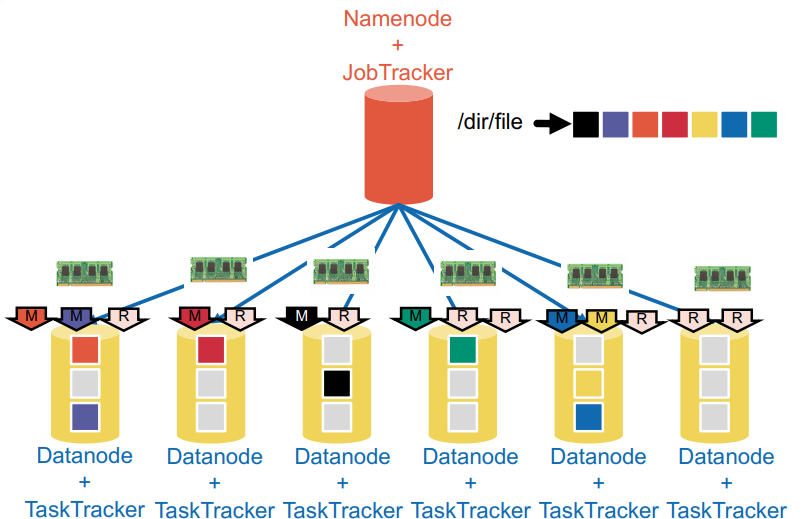
\includegraphics[width=1\linewidth]{figures/mr_mapping_phase}
		\caption{Mapping Phase}
		\label{fig:mrmappingphase}
	\end{subfigure}%
	\begin{subfigure}[t]{.3\textwidth}
		\centering
		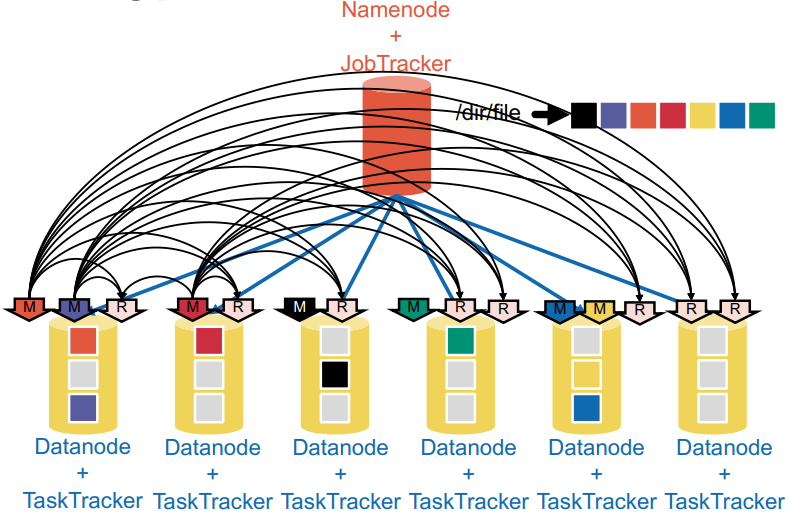
\includegraphics[width=1\linewidth]{figures/mr_shuffling_phase}
		\caption{Shuffling Phase}
		\label{fig:mrshufflingphase}
	\end{subfigure}
	\begin{subfigure}[t]{.3\textwidth}
		\centering
		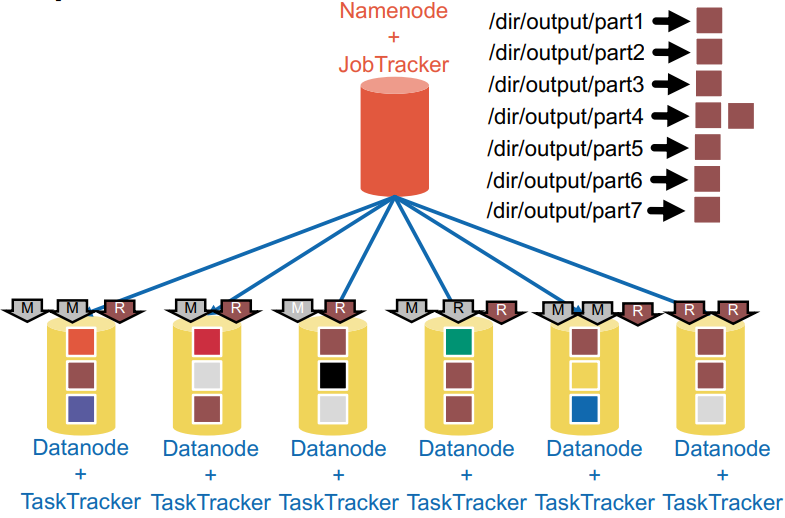
\includegraphics[width=1\linewidth]{figures/mr_reduce_phase}
		\caption{Reduce Phase}
		\label{fig:mrreducephase}
	\end{subfigure}
	\caption{MapReduce phases}
\end{figure}

\subsection{Input/output format}

How do we create key-value pairs? We can have different inputs: tables (HBase, RDBMS, ...), files (JSON, XML, ...), etc. There is an intrinsic way to convert each data shape into key-value format.

\begin{compactitem}
\item Tabular: Use primary key (RDBMS), row ID (HBase) as key and the rest of the row (all attribute values) as value $\rightarrow$ key-value pair.
\item Text: different possibilities, e.g. use line number as key and text line as value.
\item Key-value: already key-value.
\item SequenceFile: binary version of a key-value file, stores generic key-values in Hadoop binary format. This is easy since it's already a key-value file, just encoded in binary.
\end{compactitem}

Example: count words in text. Map every line number to text. Even easier: map each single word in text (key) to count 1 (value). Mappers will collect all keys (words) in their splits and sum up the 1-counts. Reducers will then collect all IR counts and sum them up.

Example: filter lines with less than 2 words out. Input: line number as key, line as value. Mapping function: filter all lines with less than 2 words out. Reduce function: identity function.


\subsection{Optimization}

We can optimize the shuffling phase by "pre-reducing" (=combine) the intermediate key-values values from the input mapping. This reduces the amount of data that needs to be shuffled around, which makes MapReduce more efficient. For example, in the word count use case, we could already count words that appear multiple times in one line and create one KV with the count. This combining can be done when spilling intermediate KVs to disk.

Often (90\%) the combine function and the reduce function are equivalent. We thus need two assumptions to hold:

\begin{compactitem}
\item Key/Value types must be identical for reduce input and output.
\item Reduce function must be commutative (a+b=b+a) and associative (a+(b+c)=(a+b)+c).
\end{compactitem}

\newpage

\subsection{MapReduce: the APIs}

Hadoop MapReduce supports a native Java API and a streaming API that allows you to write your map and reduce functions in languages other than Java. Hadoop Streaming uses Unix standard streams as the interface between Hadoop and your program, so you can use any language that can read standard input and write to standard output to write your MapReduce program.


\subsection{Tricky point: blocks and splits}

Split vs map tasks: a split is essentially an HDFS block. But in HDFS, a block is just 128MB long and then cut $\rightarrow$ you may separate a value into two blocks. HDFS only sees binary data and does not differentiate key/value borders.

MapReduce solves this by doing the splits on a more logical level, i.e. a split always includes the whole last key-value. The problem now is that the last key-value of one split could be in two different blocks. This is generally not an issue (just read the other block) except when the other block that contains the rest of the last key-value pair is remote (on another machine). This then requires a remote read, which leads to a slight decrease in performance, but MapReduce will take care of this.

\subsection{Reading Assignment}

\subsubsection{Hadoop: The definitive guide}

\textbf{Example}: find the maximum global temperature record for each year from weather data. This can be done using MapReduce. The input mapping is just a (line-offset, weather measurement) key-value pair. The mapping function extracts a (year, temperature) key-value pair for each weather record. The reduce function finally returns the maximum temperature in a key-value pair (year, [temperatures]), where [temperature] is an array temperatures for all measurements of that year.

\begin{figure}[hb!]
	\centering
	\includegraphics[width=0.7\linewidth]{figures/mr_reading_weather_example}
	\caption{MapReduce example: finding the hottest temperature for each year}
	\label{fig:mrreadingweatherexample}
\end{figure}

\textbf{Data Flow:} A MapReduce job is a unit of work that the client wants to be performed: it consists of the input data, the MapReduce program, and configuration information. Hadoop runs the job by dividing it into tasks, of which there are two types: map tasks and reduce tasks. The tasks are scheduled using YARN and run on nodes in the cluster. If a task fails, it will be automatically rescheduled to run on a different node. Hadoop divides the input to a MapReduce job into fixed-size pieces called input splits, or just splits. Hadoop creates one map task for each split, which runs the user-defined map function for each record in the split. Smaller splits are preferred since they allow for better load balancing and thus more efficient use of resources. On the other hand, if splits are too small, the overhead of managing the splits and map task creation begins to dominate the total job execution time. For most jobs, a good split size tends to be the size of an HDFS block, which is 128 MB by default, although this can be changed for the cluster (for all newly created files) or specified when each file is created.

\subsubsection{MapReduce: Simplified Data Processing on Large Clusters}

\textbf{Fault tolerance:}

\begin{compactitem}
\item Worker failure: The master (JobTracker) pings workers (TaskTracker) periodically. If no response is received from a worker in some amount of time, the worker is marked failed and the map task is reset back to idle.
\item Master failure: It is easy to make the master write periodic checkpoints of the master data structures described above. If the master task dies, a new copy can be started from the last checkpointed state.
\end{compactitem}

\newpage

\section{Resource Management}

There are some issues with MapReduce 1 that YARN addresses:

\begin{compactitem}
\item Scalability: MapReduce 1 only works with $<$4000 nodes and $<$ 40'000 tasks.
\item Bottleneck on the JobTracker: the JobTracker has too many responsibilities. The JobTracker needs to do resource management, scheduling, monitoring, job life-cycle, fault tolerance - a lot of things and there is only one JobTracker.
\item Jack of all trades, master of none: JobTracker is not specialized and thus not efficient since it needs to do so many different things.
\item Static allocation, fixed size: Map \& Reduce slots are assigned statically at configuration time (i.e. before the job starts), which leads to them often being idle, which does not fully use cluster resources.
\item Not fungible: Reduce slots are idle during map phase and map slots are idle during reduce phase.
\item Need for non-MapReduce workloads. Ability to share cluster with MPI, graph processing, and any user code.
\item Agility. Ability to maintain MapReduce frameworks of different versions.\\
\end{compactitem}

\subsection{YARN (Yet Another Resource Negotiator)}

YARN is a resource management tool that separates the JobTrackers responsibilities. The responsibilities are split into:

\begin{compactitem}
\item Resource Manager: Scheduling, Application management
\item Application masters (many): Monitoring
\end{compactitem}

YARN can be used for many applications: MapReduce, DAG distributed processing, message passing interface, graph processing. Further, YARN scales better (10'000 nodes, 100'000 tasks).


\subsubsection{YARN architecture}

Again, we use a master-slave architecture. We have the ResourceManager (RM) as master and NodeManagers (NM) as slaves. The ResourceManager acts as the central authority arbitrating resources among
various competing applications in the cluster (decides who gets which container). The NodeManager is the “worker” daemon in YARN. It authenticates container leases, manages containers’ dependencies, monitors their execution, and provides a set of services to containers. The NM will also kill containers as directed by the RM or the AM. We further have the notion of slots again, here called \textit{containers}. Containers do the virtualization of resources, mapping and reducing will be done in containers. This allows for more fine grained resource requests (memory and CPU only for now). Communications between RM and NMs are heartbeatbased for scalability. Application Masters (AM) are the "head" of a job, managing all lifecycle aspects including dynamically increasing and decreasing resources consumption, managing the flow of execution (e.g., running reducers against the output of maps), handling faults and computation skew, and performing other local optimizations. The AM is the process that coordinates the application’s execution in the cluster, but it itself is run in the cluster just like any other container. \\

\begin{figure}[hb!]
	\centering
	\begin{subfigure}[t]{.5\textwidth}
		\centering
		\includegraphics[width=0.8\linewidth]{figures/yarn_1}
		\label{fig:yarn1}
	\end{subfigure}%
	\begin{subfigure}[t]{.5\textwidth}
		\centering
		\includegraphics[width=0.8\linewidth]{figures/yarn_2}
		\label{fig:yarn2}
	\end{subfigure}
	\caption{YARN}
\end{figure}

\textbf{YARN process:} When a client submits a job, it is first sent to the RM. The RM then distributes the containers. The RM then allocates an AM (can be different for every machine) - the Application Master takes care of monitoring. The AM requests resources (containers) from the RM. Typically, an AM will need to harness the resources (CPUs, RAM, disks etc.) available on multiple nodes to complete a job. To obtain resources (containers), AM issues resource requests to the RM.  The NM only assigns containers locally, the Application Master needs the authorization from the Resource Manager. When a resource is allocated on behalf of an AM, the RM generates a lease for the resource, which is pulled by a subsequent AM
heartbeat.  At the beginning, the AM only requests mapping resources. Once mapping is done, only then does it request reducing resources.

The resulting process is then essentially MapReduce with YARN around it.

The ResourceManager is a pure scheduler, it does not monitor tasks and it does not restart upon failure. Different scheduling strategies exist:

\begin{compactitem}
\item FIFO scheduler: First applications has priority. Problem: long running applications can block small ones.
\item Capacity scheduler: Have several queues, every queue gets separate part of the cluster.
\item Hierarchical queues (Steady Fair Share)
\item Fair scheduler: idle clusters are temporarily reassigned while idle. Preempted when original job needs resources. 
\end{compactitem}

Note: people say MapReduce and Spark are slow. But: these technologies are not built to minimize latency but to maximize cluster optimization.

\subsection{Reading assignment: Apache Hadoop YARN: Yet Another Resource Negotiator}

\begin{compactitem}
\item The ResourceManager exposes two public interfaces towards: 1) clients submitting applications, and 2) ApplicationMaster(s) dynamically negotiating access to resources, and one internal interface towards NodeManagers for cluster monitoring and resource access management.
\item The AM periodically heartbeats to the RM to affirm its liveness and to update the record of its demand. After building a model of its requirements, the AM encodes its preferences and constraints in a heartbeat message to the RM.
\end{compactitem}



\newpage

\section{Distributed Computations II: Spark}

\subsection{Introduction to Spark}

Both MapReduce 1 and MapReduce 2 (YARN) use a rather restricted data flow model: data is first mapped to an intermediate representation and then reduced to an output. This is a very specific topology (\textit{not} DAG-based). Spark is capable of much more because it supports any DAG data flow. Let's build something much more general.

\begin{figure}[hb!]
	\centering
	\begin{subfigure}[t]{.5\textwidth}
		\centering
		\includegraphics[width=0.1\linewidth]{figures/spark_mr_intuition}
		\label{fig:sparkmrintuition}
	\end{subfigure}%
	\begin{subfigure}[t]{.5\textwidth}
		\centering
		\includegraphics[width=0.4\linewidth]{figures/spark_dag_dataflow}
		\label{fig:sparkdag}
	\end{subfigure}
	\caption{MapReduce dataflow vs. DAG dataflow}
\end{figure}

Spark uses \textbf{RDDs (Resilient Distributed Dataset)} as data format. An RDD is a big collection of values (not limited to key-values!) that can be recomputed and is spread over machines. RDDs are partitioned (like MapReduce uses splits).

\textbf{RDD lifecycle:} RDDs can be created on the fly from data in HDFS - RDD is just the data read from HDFS and partitioned along HDFS blocks. RDDs can be transformed into other RDDs (many-to-many transform) (like mapping/reducing in MapReduce). An RDD is only returned (output) once an action is taken on the RDD. RDDs and their transforms can be represented by a directed acyclic graph (DAG) where nodes are RDDs and egdes are transformations. This lineage graph uses lazy evaluations - nothing happens (no transformations are executed) until an action is requested at some RDD. Only then will the data flow through the graph and be transformed and output. Spark can be executed in application or shell.

\begin{figure}[hb!]
	\centering
	\includegraphics[width=0.25\linewidth]{figures/spark_hello_world}
	\caption{Example program in Spark}
	\label{fig:sparkhelloworld}
\end{figure}


\subsection{Spark: overview of transformations}

As we've seen, RDDs can be transformed. Many different ($\sim$100) transformations exist.

\textbf{Transformation on one RDDs:}
\begin{compactitem}
\item filter: eliminate values that don't fulfill some test (= SELECTION in rel. algebra). Narrow dependency.
\item map: map each value in input to some value in output (\#input values = \#output values). Narrow dependency.
\item flatMap: Map to multiple outputs, but outputs are flattened. Narrow dependency.
\item distinct: eliminate duplicates/ Wide dependency.
\item sample: pick inputs randomly.
\end{compactitem}

\begin{figure}[t!]
	\centering
	\begin{subfigure}[t]{.3\textwidth}
		\centering
		\includegraphics[width=0.7\linewidth]{figures/spark_filter}
		\caption{filter}
	\end{subfigure}%
	\begin{subfigure}[t]{.3\textwidth}
		\centering
		\includegraphics[width=0.7\linewidth]{figures/spark_map}\
		\caption{map}
	\end{subfigure}
	\begin{subfigure}[t]{.3\textwidth}
		\centering
		\includegraphics[width=0.7\linewidth]{figures/spark_flatmap}
		\caption{flatmap}
	\end{subfigure}
\end{figure}

\begin{figure}[t!]
	\centering
	\begin{subfigure}[t]{.3\textwidth}
		\centering
		\includegraphics[width=0.7\linewidth]{figures/spark_distinct}
		\caption{filter}
	\end{subfigure}%
	\begin{subfigure}[t]{.3\textwidth}
		\centering
		\includegraphics[width=0.7\linewidth]{figures/spark_sample}\
		\caption{map}
	\end{subfigure}
\end{figure}

\textbf{Transformation on two RDDs:}
\begin{compactitem}
\item union
\item intersection
\item substract
\item cartesian product
\end{compactitem}

\begin{figure}[hb!]
	\centering
	\begin{subfigure}[t]{.21\textwidth}
		\centering
		\includegraphics[width=0.7\linewidth]{figures/spark_union}
		\caption{union}
	\end{subfigure}%
	\begin{subfigure}[t]{.21\textwidth}
		\centering
		\includegraphics[width=0.7\linewidth]{figures/spark_intersection}\
		\caption{intersection}
	\end{subfigure}
	\begin{subfigure}[t]{.21\textwidth}
		\centering
		\includegraphics[width=0.7\linewidth]{figures/spark_substract}
		\caption{substract}
	\end{subfigure}
	\begin{subfigure}[t]{.21\textwidth}
	\centering
	\includegraphics[width=0.7\linewidth]{figures/spark_cart_product}
	\caption{cartesian product}
	\end{subfigure}
\end{figure}

\newpage

\subsection{Spark: overview of actions}

\begin{compactitem}
\item collect: put RDDs into local memory/ disk. This only works when RDDs are small enough to even fit in memory/ disk (risky).
\item count
\item count by value
\item take: collect a specified number of values
\item top: return top values
\item takeSample: random values taken
\item reduce
\end{compactitem}

\subsection{Spark: pair RDDs}

We can have RDDs of values that are pairs (like MapReduce with key-values). Spark provides special operations on RDDs containing key/value pairs. These RDDs are called pair RDDs. Pair RDDs are a useful building block in many programs, as they expose operations that allow you to act on each key in parallel or regroup data across the network. 

\textbf{Transformation:}

\begin{compactitem}
\item keys: get all keys. Narrow dependency.
\item values: get all values. Narrow dependency.
\item reduce by key: group by key and output some aggregate value per key. Like reduce in MR. Wide dependency.
\item group by key: keep all values per key and group them together. Wide dependency.
\item sort by key (like GROUP BY). Wide dependency.
\item map values: map each value to another value. Narrow dependency.
\item join: combine values with same keys from two RDDs.
\item substract by key
\item count by key
\item lookup
\end{compactitem}

\newpage

\subsection{Physical layer}

We again want parallel execution. The input data is split (mostly according to HDFS blocks, short circuiting) and we have one task per block. Executors will then execute the tasks. We don't want to assign one single tasks per executor: some tasks may take longer, so that most executors will be idle waiting for the last one(s) to complete. We thus want smaller tasks that can be spread over executors such that each executor has multiple small tasks. If one executor finishes, it can just continue with the next task. Tasks are thus spread over executors and spread over CPUs within an executor. 

\begin{figure}[t!]
	\centering
	\begin{subfigure}[t]{.5\textwidth}
		\centering
		\includegraphics[width=0.7\linewidth]{figures/spark_parallelize_not_ideal}
		\caption{Suboptimal parallel execution }
	\end{subfigure}%
	\begin{subfigure}[t]{.5\textwidth}
		\centering
		\includegraphics[width=0.7\linewidth]{figures/spark_parallelize_ideal}\
		\caption{Improved parallel execution}
	\end{subfigure}
\end{figure}

\textbf{Sequence of (parallelizable) transformations:} We can further improve parallelization by grouping together series of transformations on the same level (not ancestor/child of each other) with narrow dependencies. We can group these transformations together as if they were a single transformation. This can reduce the amount of data that needs to be shuffled around. We should try to execute transformations that have dependencies on a machine on that machine, as long as the transformations allow this - compute locally as much as possible.

\begin{figure}[hb!]
	\centering
	\begin{subfigure}[t]{.3\textwidth}
		\centering
		\includegraphics[width=0.5\linewidth]{figures/spark_transformation_sequence}
		\caption{Sequence of transformations}
	\end{subfigure}%
	\begin{subfigure}[t]{.3\textwidth}
		\centering
		\includegraphics[width=0.8\linewidth]{figures/spark_transformation_sequence_ineff}\
		\caption{Inefficient allocation to executors}
	\end{subfigure}
	\begin{subfigure}[t]{.3\textwidth}
		\centering
		\includegraphics[width=0.8\linewidth]{figures/spark_transformation_sequence_eff}
		\caption{Efficient allocation to executors}
	\end{subfigure}
\end{figure}

\textbf{Stage:} We call a set of transformations that all have narrow dependencies (i.e. the transformations are parallelizable, don't require shuffling) and that can all be executed on the same executor a stage. Stages can be spread over executors/ cores.

Once we encounter a \textit{wide dependency}, the stage is finished, we need to shuffle around. A wide dependency requires all input values, which requires shuffling (send over the network). A new stage needs to be set up.\\

\textbf{Idea of Spark:} do as many narrow dependency transformations in one stage as possible, then wait until all tasks in a stage have finished and then shuffle once the stage is done. A spark job as a whole is a \textit{sequence/DAG of stages}.

\begin{figure}[hb!]
	\centering
	\includegraphics[width=0.3\linewidth]{figures/spark_job}
	\caption{Spark job}
	\label{fig:sparkjob}
\end{figure}

\textbf{Terminology}

\begin{compactitem}
\item Vertical grouping: group transformations into stage
\item Horizontal splitting: split stage into tasks
\item Sequence: arrange stages into Spark job.\\
\end{compactitem}


\subsection{Performance tuning}

Consider any DAG with multiple output RDDs. Remember that evaluation is lazy - transformation are only executed once an action is applied on an RDD. If we apply an actions to multiple RDDs that all have common ancestor RDDs, the ancestor RDDs are calculated multiple times equivalently. This is very inefficient since we keep recomputing the same RDDs over and over.\\

\textbf{Persisting RDDs:} We can instruct Spark to persist some RDDs (cache them). Considering Figure \ref{fig:sparkpersrdds}, an action on output RDDs then only requires one single transformation. After computing it the first time, Spark will store the RDD contents in memory (partitioned across the machines in your cluster), and reuse them in future actions. Persisting RDDs on disk instead of memory is also possible. If you attempt to cache too much data to fit in memory, Spark will automatically evict old partitions using a Least Recently Used (LRU) cache policy. 

\begin{figure}[t!]
	\centering
	\begin{subfigure}[t]{.5\textwidth}
		\centering
		\includegraphics[width=0.25\linewidth]{figures/spark_dag_ineff}
		\caption{Inefficient recomputation of RDDs}
	\end{subfigure}%
	\begin{subfigure}[t]{.5\textwidth}
		\centering
		\includegraphics[width=0.25\linewidth]{figures/spark_persisting_rdds}
		\caption{Spark persisiting RDDs}
		\label{fig:sparkpersrdds}
	\end{subfigure}
	\caption{}
\end{figure}

\textbf{Avoiding wide dependencies:} As we've seen, wide dependencies require shuffling, which takes time. Spark splits RDDs into partitions. What if we pre-partition the input s.t. shuffling is no longer necessary. We can tell Spark to proactively partition the data. The amount of work is the same, we just partition differently and as a result have less shuffling. Spark partitions key-values s.t. all KV pairs with the same key are already on the same machine and no shuffling is necessary.

\subsection{Data Frames}

RDDs are a low-level concept, it's just a collection of values. Doing processing on RDDs using Spark and Python is not simple. That's why we introduce DataFrames - we basically already know what they are: tables. Most important concept: data independence. Since with DataFrames we now have tables, we don't have to use transformations and actions. We can use SQL like queries which can be translated by Spark to transformations and actions. You can still use transformations on DataFrames, but SQL is generally easier to use.

If each value in an RDD is a dataset row and all values have the same set of attributes (columns), we can just interpret the RDD as a table, i.e. a DataFrame.\\

\textbf{Columnar storage:} Spark can store columns together. In a column, all values typically have the same datatype. This allows for much more efficient storing in memory. For example, a int32 column can be stored as just a multiple of 32bits $\rightarrow$ highly structured and efficient. DataFrames thus have a much lower memory footprint.

\textbf{Schema inference:} Spark automatically infers types (works for csv, json, ...).\\

It is possible to convert back and forth between DataFrames and RDDs, however in practice it is best to just stick with one and don't mix.

\textbf{Limits of DataFrames: Heterogeneity}\\
In practice, we don't have uniform data, e.g. column \textit{foo} might be int somewhere but an array somewhere else. Then forcing the values into a column will produce all strings (e.g. "1" and "[1,2]").

\subsubsection{Dealing with nestedness}

As we've seen, JSON and XML don't always fit into tables since they allow nested data. Thus, transformations are still useful since if our data is not in tables, we can't use SQL. Then we need transformations.

Spark also offers additional optimizations to deal with nested data:

\begin{compactitem}
\item Arrays: Spark offers an \textit{explode()} function that automatically expands an array into normal form. We essentially get one single row for each value in the array.
\item Objects: Spark allows accessing fields of objects using SQL, using a '.' notation (like class attribute). This allows us to explore tables with objects in them. 
\end{compactitem}

\begin{figure}[t!]
	\centering
	\begin{subfigure}[t]{.5\textwidth}
		\centering
		\includegraphics[width=0.9\linewidth]{figures/spark_nestedness_arrays}
	\end{subfigure}%
	\begin{subfigure}[t]{.5\textwidth}
		\centering
		\includegraphics[width=0.9\linewidth]{figures/spark_nestedness_objects}
	\end{subfigure}
\end{figure}

\newpage

\subsection{Apache Spark Architecture (Exercise)}

Spark is a cluster computing platform designed to be fast and general purpose. Spark extends the MapReduce model to efficiently cover a wide range of workloads that previously required separate distributed systems, including interactive queries and stream processing. Spark offers the ability to run computations in memory.
At a high level, every Spark application consists of a driver program that launches various parallel operations on a cluster. The driver program contains your application's main function and defines distributed datasets on the cluster, then applies operations to them.

Driver programs access Spark through a SparkContext object, which represents a connection to a computing cluster. There is no need to create a SparkContext; it is created for you automatically when you run the first code cell in the Jupyter. The driver communicates with a potentially large number of distributed workers called executors. The driver runs in its own process and each executor is a separate process. A driver and its executors are together termed a Spark application.


\subsection{PySpark API}

Commonly used transformations:

\begin{compactitem}
\item \texttt{filter()} returns a new RDD containing only the elements that satisfy a predicate.
\item \texttt{map()} returns a new RDD by applying a function to each element of this RDD.
\item \texttt{distinct()} returns a new RDD containing the distinct elements in this RDD.
\item \texttt{sortBy()} sorts the RDD by the given keyfunc.
\item \texttt{groupByKey()} groups the values for each key in the RDD into a single sequence.
\item \texttt{groupBy()} returns an RDD of grouped items.
\item \texttt{reduceByKey()} merges the values for each key using an associative and commutative reduce function.
\item \texttt{mapValues()} passes each value in the key-value pair RDD through a map function without changing the keys; this also retains the original RDD’s partitioning.
\end{compactitem}

Commonly used actions:

\begin{compactitem}
\item \texttt{count()} returns the number of elements in the RDD.
\item \texttt{collect()} returns a list that contains all of the elements in this RDD.
\item \texttt{countByKey()} counts the number of elements for each key, and return the result to the master as a dictionary.
\item \texttt{countByValue()} returns the count of each unique value in this RDD as a dictionary of (value, count) pairs.
\end{compactitem}



In the following, we show a set of example queries using pyspark on \textit{The Great Language Game} dataset. An entry has the following structure:

\begin{lstlisting}[basicstyle=\small,columns=flexible]
[
 {
  "guess": "German",
  "target": "German",
  "country": "AU",
  "choices": ["German", "Serbian", "Swedish", "Vietnamese"],
  "sample": "e77d97b712adffc39e531e20237a5589",
  "date": "2013-08-19"
 }
]
\end{lstlisting}

Find all games such that the guessed language is correct (=target), and such that this language is Russian. How long is the resulting sequence?

\begin{lstlisting}[language=Python,basicstyle=\small,columns=flexible]
match = entries.filter(lambda e: e['guess'] == e['target'] and e['target'] == 'Russian').count()
\end{lstlisting}



For those cases where the guess matched the target, list what the guessed language was.  How many times was Hindi correctly guessed?

\begin{lstlisting}[language=Python,basicstyle=\small,columns=flexible]
matching = entries.filter(lambda e: e['guess'] == e['target'] == 'Hindi').count()
\end{lstlisting}

Find all distinct values of the target languages (i.e. the target field). How many distinct languages are there?

\begin{lstlisting}[language=Python,basicstyle=\small,columns=flexible]
matching = entries.map(lambda e: (e['target'])).distinct().count()
\end{lstlisting}

Return the top three games where the guessed language is correct (=target) ordered by language (ascending), then country (ascending), then date (ascending).

\begin{lstlisting}[language=Python,basicstyle=\small,columns=flexible]
matching = entries.filter(lambda e: e['guess'] == e['target'])
matching = matching.sortBy(lambda e: (e['target'], e['country'], e['date'])).take(3)
\end{lstlisting}

Aggregate all games by country and target language, counting the number of guessing games that were done for each pair (country, target).

\begin{lstlisting}[language=Python,basicstyle=\small,columns=flexible]
matching = entries.map(lambda e: (e['country']+e['target'])).countByValue()
\end{lstlisting}

Among all the games where the guess was correct (=target), what is the percentage of cases where the first choice (among the array of possible answers) was the target?

\begin{lstlisting}[language=Python,basicstyle=\small,columns=flexible]
correct = entries.filter(lambda e: e['guess'] == e['target'])
perc = correct.filter(lambda e: e['choices'][0] == e['target']).count() / correct.count()
\end{lstlisting}

For each target language, compute the percentage of successful guess games (i.e. guess == target) relative to all games for that target language, and display the pairs (target\_language, percentage) in ascending order of the percentage.

\begin{lstlisting}[language=Python,basicstyle=\small,columns=flexible]
outcomes = entries.map(lambda e: (e['target'], e['target'] == e['guess'])).groupByKey()
matching = outcomes.mapValues(lambda e: float(list(e).count(True)/len(e)))
matching = matching.sortBy(lambda e: e[1], ascending=False).take(3)
\end{lstlisting}

Group the games by the index of the correct answer in the choices array and output all counts.

\begin{lstlisting}[language=Python,basicstyle=\small,columns=flexible]
matching = entries.map(lambda e: e['choices'].index(e['target'])).countByValue()
\end{lstlisting}

For the cases where the guess matched the target and target = 'French', report what is the count of each possible number of choices (e.g. if you have 2 games where there are 3 possible choices, then you should report something like (3, 2) for this number of choices). 

\begin{lstlisting}[language=Python,basicstyle=\small,columns=flexible]
matching = entries.filter(lambda e: e['guess'] == e['target'] == 'French')
matching = matching.map(lambda e: len(e['choices'])).countByValue()
\end{lstlisting}

What is the language of the sample that has the highest successful guess rate?

\begin{lstlisting}[language=Python,basicstyle=\small,columns=flexible]
def perc(l):
    tot = len(l)
    corr = list(l).count(True)
    return corr/tot
matching = entries.map(lambda e: (e['sample']+e['target'], e['guess'] == e['target'])).groupByKey()
matching = matching.mapValues(perc).sortBy(lambda e: e[1], ascending=False).take(3)
\end{lstlisting}

Return all games played on the latest day.

\begin{lstlisting}[language=Python,basicstyle=\small,columns=flexible]
matching = entries.map(lambda e: (e['date'], 1)).reduceByKey(lambda x,y: x+y)
matching = matching.sortBy(lambda e: e[0], ascending=False).take(3)
\end{lstlisting}

\subsection{Dataframes and SparkSQL}

Spark Dataframes allow the user to perform simple and efficient operations on data, as long as the data is structured and has a schema. Dataframes are similar to relational tables in relational databases: conceptually a dataframe is a specialization of a Spark RDD with schema information attached. 

\newpage

\section{Document stores}

Documents are just trees. Document stores are often referred to as NoSQL (= not only SQL).\\

\textbf{Remember: relational model}\\
Typical relational stack: bits $\rightarrow$ text $\rightarrow$ well-formed CSV $\rightarrow$ relational schema $\rightarrow$ queryable tables.

Relational tables fulfill relational integrity (all rows have the same columns), atomic integrity (no nested tables), domain integrity (strict type per column). Relational algebra provides a way to query data with SQL being an easy query language.

Remember: We want to rebuild that stack for clusters. Up until now, we have rebuilt the stack for tables on clusters. Now: we want to do the same for the tree data model.

\begin{figure}[hb!]
	\centering
	\begin{subfigure}[t]{.3\textwidth}
		\centering
		\includegraphics[width=0.6\linewidth]{figures/docstores_structured_stack}
		\caption{The structured stack}
	\end{subfigure}%
	\begin{subfigure}[t]{.3\textwidth}
		\centering
		\includegraphics[width=0.6\linewidth]{figures/docstores_semistructured_stack}
		\caption{The semi-structured stack}
	\end{subfigure}
	\begin{subfigure}[t]{.3\textwidth}
		\centering
		\includegraphics[width=0.6\linewidth]{figures/docstores_mongodb_stack}
		\caption{The MongoDB stack}
	\end{subfigure}
\end{figure}

\subsection{Making trees fit into tables}

Why not reuse things? We could try to fit trees into tables.

For flat trees, this is definitely possible (e.g. a tree with just leafs is just a row). We can natively fit several flat trees as several rows into a table, for both JSON and XML. However, all flat trees need the same fields (columns) and the same data type for each field. How do we ensure this domain integrity? We can use schemas! We can validate JSON or XML by using schemas and thus make sure that the trees are flat trees with all the same fields and domain integrity.\\

We thus can fit trees into tables, but we need to assume a lot: relational integrity (all same fields), atomic integrity (flat trees), maybe domain integrity (all same type in one column). For trees, this is generally not the case.

In general, we have \textbf{nestedness} and \textbf{heterogeneity}. Could we solve this...?

Nested arrays: there are ways to fix it, use multiple tables, explode row.

Heterogeneity: put NULL in missing fields.

However, this is not a good solution. \textbf{Impedance mismatch:} data to store does not have the same shape as the storage. This is why we have document stores.

\subsection{Document stores (MongoDB)}

\textbf{Characteristics:}

\begin{compactitem}
\item Document stores don't scale as well as MapReduce, Spark, HDFS, etc. MongoDB works on a few machines (not 1000s). 
\item A document store is a collection of trees (large number of small trees). You can have bigger documents (e.g. picture, MB size), but not documents in the GB or TB region.
\item Document stores store millions or billions of such small documents. AND: the documents don't need to look alike (but often they do).
\item Tree vs. flat: document stores natively support nestedness where as rel. DBs are flat.
\item Homogeneous vs. Heterogeneous: document stores natively support heterogeneity (every column/field can look different) where as rel. DBs are homogeneous (everything needs to be equivalent).
\item Document stores support SQL principles such as Projection, Selection, Aggregation. BUT: joins are not ideal, very expensive (you can still implement your own join). This is not really an issue though because the data is denormalized $\rightarrow$ we already "precomputed" the joins by nesting the data.
\item NoSQL: validation \textit{after} the data was populated $\rightarrow$ validation on read (compared to RDBMS where schema needs to specified first $\rightarrow$ schema on write).
\end{compactitem}

\textit{Many} document stores implementations exist (MongoDB, CouchDB, elasticsearch, etc.) We focus on MongoDB. MongoDB uses JSON (document stores using XML exist as well). But MongoDB supports more types than JSON (dates, binary, etc.). MongoDB stores JSON documents as binary, which is more efficient: BSON (binary JSON). MongoDB thus does not have text, it stores directly into BSON. 

\subsection{Querying a document store}

Ideally, we'd want to query document stores with a language like SQL. On a lower level, we need a CRUD (create, read, update, delete) based access to the document store. SQL (query language) can then build on top of this and provide easy querying for users.\\

\begin{table}[hb!]
\centering
\begin{tabular}{|p{20mm}|p{75mm}|p{75mm}|}
	\hline 
	Desc & Low level query & SQL equivalent\\ 
	\hline 
	Read & db.scientists.find(\{"Theory": "Relativity"\}) & SELECT * FROM scientists
	WHERE Theory = "Relativity" \\ 
	\hline 
	Read: projection & db.scientists.find(\{ "Theory": "Relativity"\},
	\{ "Name" : 1, "Last": 1 \}
	) & SELECT Name, Last
	FROM scientists
	WHERE Theory = "Relativity" \\ 
	\hline 
	Read: AND & db.scientists.find(\{"Theory": "Relativity", "Last": "Einstein"\}, \{ "Name" : 1, "Last": 1 \}) & SELECT Name, Last
	FROM scientists
	WHERE Theory = "Relativity"
	AND Last = "Einstein" \\ 
	\hline 
	Read: OR & db.scientists.find(
	\{\$or : [\{ "Last" : "Newton" \},	\{"Last": "Einstein" \}]\}) & SELECT *
	FROM scientists
	WHERE Last = "Newton"
	OR Last = "Einstein" \\ 
	\hline 
	Read: Comparison & db.scientists.find(\{"Publications": \{\$gte: 100\}\}) & SELECT *
	FROM scientists
	WHERE Publications $>$= 100 \\ 
	\hline 
\end{tabular}
\end{table}


These low level queries further support heterogeneity, i.e. they still work if we have missing fields or different types. Further, these queries support nestedness, which SQL does not.

\begin{table}[hb!]
\centering
\begin{tabular}{|p{40mm}|p{135mm}|}
	\hline 
	\textbf{Desc} & \textbf{Low level query} \\ 
	\hline 
	Read: nestedness (objects) & db.scientists.find(\{"Name.First": "Albert"\}) \\ 
	\hline 
	Read: nestedness (arrays) & db.scientists.find(\{"Theories": "Special relativity"\}) \\ 
	\hline 
	Read: other operators & db.scientists.find(\{"University": \{\$in: ["ETH Zurich", "EPFL"]\}\}) \\ 
	\hline 
	Count & db.scientists.find(\{"University": \{\$in: ["ETH Zurich", "EPFL"]\}\}).count() \\ 
	\hline 
	Sort (-1: descending) & db.scientists.find(\{"University": \{\$in: ["ETH Zurich", "EPFL"]\}\}).sort(\{"Founded": -1\}) \\ 
	\hline 
	Limit and offset & db.scientists.find(\{"University": \{\$in: ["ETH Zurich", "EPFL"]\}\}).sort(\{"Founded": -1\}).skip(30).limit(10) \\ 
	\hline 
	Duplicates & db.scientists.distinct("name") \\ 
	\hline 
	Access array element & db.scientists.find(\{"Theories.0": "Special relativity"\}) \\
	\hline
\end{tabular} 
\end{table}

Possible confusion: \texttt{db.scientists.find(\{"Name.First": "Albert"\})} finds all documents where the "First" field of the "Name" object is "Albert". \texttt{db.scientists.find(\{"Name": \{"First": "Albert"\}\})} however searches for the \textit{exact} object "Name" of form \texttt{\{"First": "Albert"\}}.

Note on \textit{Read: nestedness (arrays)}: If we have an array, just searching for \texttt{\{"Theories": "Special relativity"\}} works, this will check if "Special relativity" is in the array "Theories".

Many other operators exist: \$nin, \$eq, \$ne, \$gt, \$lt, \$lte,...

There also exist aggregation and pipelines (like in Spark). But there is an easier way to do this (see section 13).

\begin{figure}[b!]
	\centering
	\includegraphics[width=0.4\linewidth]{figures/docstores_aggregation_pipeline}
	\caption{Aggregation and pipelines}
	\label{fig:docstoresaggregationpipeline}
\end{figure}

\textbf{Data defintion:} Observe that we can find existing docs and update them. This is not possible in Spark and HDFS.

\begin{table}
\centering
\begin{tabular}{|c|c|}
	\hline 
	\textbf{Desc} & \textbf{Low level query} \\ 
	\hline 
	Insert & db.scientists.insertOne(\{"Name": "Einstein", "Theory": "Relativity"\}) \\ 
	\hline 
	Update & db.scientists.updateMany(\{"Name": "Einstein"\},
	{ \$set: {"Century": "20"}}) \\ 
	\hline 
	Remove & db.scientists.deleteMany(\{"century": "15"\}) \\ 
	\hline 
\end{tabular} 
\end{table}


Document stores are document write atomic (like HBase: row atomic). Two users can't write to the same document simultaneously.

\subsection{Architecture}

Principles of big data:  Shard the data, Replicate the data,  Buy lots of cheap hardware. MongoDB does this as well. However, typically we don't have lots of shards and only few machines.

\begin{figure}[hb!]
	\centering
	\begin{subfigure}[t]{.5\textwidth}
		\centering
		\includegraphics[width=0.6\linewidth]{figures/docstores_clustering}
		\caption{Clustering model}
	\end{subfigure}%
	\begin{subfigure}[t]{.5\textwidth}
		\centering
		\includegraphics[width=0.8\linewidth]{figures/docstores_clustering_phys}
		\caption{Clustering on the physical level}
	\end{subfigure}
\end{figure}

We, again, have a master-slave architecture. One master replica and several slave replicas. An important feature of document stores is the ability to modify data (not possible in Spark, MapReduce, ...). When writing, the write goes to the master, which will execute it and forward the write to all slave replicas. The slaves send ACKs. However, in order to speed writing up, the master only waits for a subset of slaves to send their ACK (the number of ACKs to wait for can be specified in MongoDB).

\subsection{Indices}

Imagine a collection of billions of objects and we start a query. Query can be of two different types:

\begin{compactitem}
\item Point query (= highly-filtering queries): returns only very few objects from the collection.
\item Not highly-filtering queries: returns lots of objects from the collection.
\item Range queries: return objects that fit into some range.
\end{compactitem}

Indices are mainly interesting for point and range queries since returning many objects is slow anyways. Thanks to indices, point queries can run in milliseconds. On Spark, which does not have indices, this would take a while (seconds to minutes).\\ 

\textbf{Indices - the principle:} Indices are like an index in a book. They directly point to an entry (object) and thus make lookups faster. Two kinds of indices exist in MongoDB: hash indices and B+ trees.


\subsubsection{Hash indices}

Hash indices are the fastest and can be created on some field by \texttt{db.scientists.createIndex(\{"Century": "hash"\})}. The procedure works as follows: the value of the specified field is hashed for every object. In a hash table, we then map the hashed value to an array of records that point to all objects that have the specified field equal to the value of that hash table entry. This allows to quickly find all objects that have a specified value in the field (e.g. all objects with "Century" 19 $\rightarrow$ lookup h(19)).

\begin{figure}[b!]
	\centering
	\includegraphics[width=0.45\linewidth]{figures/docstores_hash_indices}
	\caption{Hash indices (the fastest)}
	\label{fig:docstoreshashindices}
\end{figure}

\textbf{Limitations of hash indices:}

\begin{compactitem}
\item No support for range queries
\item Hash function not perfect in real life
\item Space requirements for collision avoidance
\end{compactitem}


\subsubsection{B+ trees indices}

B+ trees are another way to index and they solve some issues of hash indices, but they are slower. Consider the B+ tree example in Figure \ref{fig:docstoresbplusex} where we group words together such that we have single disk read $\rightarrow$ less latency. B+ trees have several keys per node. These values define intervals (e.g. 2 keys: 3 intervals = 3 children, 4 keys: 5 intervals = 5 children). For each interval, there is a child. In B+ trees, all leaves have the same depth and all non-leaf nodes have between d+1 and 2d+1 children (the root can have less).

\begin{figure}[hb!]
	\centering
	\includegraphics[width=0.5\linewidth]{figures/docstores_bplus_ex}
	\caption{B+ tree example}
	\label{fig:docstoresbplusex}
\end{figure}

\textbf{Procedure:} We keep inserting into an empty tree. First, all values just go in the root. Once we have more than 4 values, we split the root and create two leafs and the last value before splitting is added as new key. This is done recursively - every time a leaf has too many values, it is split. If the parent has not yet too many keys, a new key is added to the parent and the leaf is split into two. If the parent already has full keys, the parent is split and a new root is added (see slides for example construction).

B+ trees can then be used to build an index, where the values for a field are entered in the tree and each value point to a set of objects. When executing a query, we just have to walk the tree. Further, B+ trees naturally encode intervals, which speeds up range queries.\\\\


MongoDB has a special field \texttt{\_id}, which always exists for any object. MongoDB always builds an index on this field, which allows for very fast lookups on the \_id field. We thus have two types of indices in MongoDB:

\begin{compactitem}
\item Primary: \_id
\item Secondary: other fields. MongoDB will only build an index for other fields if instructed to do so.
\end{compactitem}

Querying without an index requires scanning through the entire collection in memory, which is very slow. With an index, we can directly \textit{prefilter} the collection without even looking at the collection. Building the index takes a while in the beginning, however once it is done, queries are very fast.\\

\subsection{Examples}

\textbf{Index (hash):} db.scientists.createIndex(\{"Name.Last": "hash"\})\\
\textbf{Query:} db.scientists.find(\{"Name.Last": "Einstein"\}) - very fast.\\

\textbf{Index (hash):} db.scientists.createIndex(\{"Profession": "hash"\})\\
\textbf{Query:} db.scientists.find(\{"Profession": "Physicist", "Theories": "Relativity"\}) - very fast, collection can be prefiltered on "Profession" (using indices) and then postfiltered in memory on "Theories".\\

\textbf{Index (compound (only B+-tree!)):} db.scientists.createIndex(\{"Birth": 1, "Death" : 1\})\\
\textbf{Query:} db.scientists.find(\{"Birth": 1887, "Death": 1946\}) - very fast.\\

\textbf{Index (compound (only B+-tree!)):} db.scientists.createIndex(\{"Birth": 1, "Death" : -1\})\\
\textbf{Query:} db.scientists.find(\{"Birth": 1887\}) - faster as well, even though it only looks at "Birth" not "Death".\\

\newpage

\textbf{Index (compound (only B+-tree!)):} db.scientists.createIndex(\{"Birth": 1, "Death" : -1\})\\
\textbf{Query:} db.scientists.find(\{"Birth": \{"\$gte" : 1980\}\}) - very fast.\\

\textbf{Index (compound (only B+-tree!)):} db.scientists.createIndex(\{"Birth": 1, "Death" : -1\})\\
\textbf{Query:} db.scientists.find({"Death" : 1887) - \textit{not fast} because the index first sorts on "Birth", then on "Death". The query only checks the second field.\\

\subsection{MongoDB: commonly used operators and commands}

\textbf{Operators:}

\begin{compactitem}
\item \texttt{\$elemMatch}: matches documents that contain an array field with at least one element that matches all the specified query criteria.
\item \texttt{\$all}: selects the documents where the value of a field is an array that contains all the specified elements.
\end{compactitem}

\subsection{Exercise}

What are advantages of document stores over relational databases?  Flexibility. Not every record needs to store the same properties. New properties can be added on the fly (Flexible schema).

Can the data in document stores be normalized? Yes. References can be used for data normalization.

How does denormalization affect performance? All data for an object is stored in a single record. In general, it provides better performance for read operations (since expensive joins can be omitted), as well as the ability to request and retrieve related data in a single database operation. In addition, embedded
data models make it possible to update related data in a single atomic write operation.

\newpage

\section{Querying trees}

In document stores, we have large collections of small trees and we can query with nested and heterogeneous data. We now want a querying layer above the data store (document store) in the stack.\\

\textbf{Data independence:} We want a logical data model with a query language independent of the physical implementation. The physical layer can be changed while the logical layer stays. For example, Spark SQL allows to query Spark using an SQL-like language, while on the physical level, Spark translates the SQL queries to transformations and actions. Due to data independence, this translation needs to be done only once, not everytime by the user.\\

However, we've seen that nested and heterogeneous data is still a problem for SQL. Using DataFrames, Spark SQL provides possible ways to deal with nestedness (explode arrays) or heterogeneity (convert everything to string) but the approach is suboptimal. We want a language that is similar to SQL but handles nestedness and heterogeneity natively $\rightarrow$ \textbf{JSONiq} (others exist).\\

Declarative language: declare \textit{what} you want (e.g. I want a cake) - vs. imperative language: declare how you want it (e.g. put sugar, flour, etc. in and bake for 30min).

Functional language: everything transforms (functions) several instances into an instance.

Set-based languages: always returns collections (e.g. rows).\\

\textbf{Language ecosystem:}

\begin{table}[hb!]
\begin{tabular}{|c|c|c|}
	\hline 
	& \textbf{XML} & \textbf{JSON} \\ 
	\hline 
	Navigation & XPath & JSONPath,
	JSONSelect \\ 
	\hline 
	Transform & XSLT & JSONT \\ 
	\hline 
	Query & XQuery 1.0/3.0 & XQuery 3.1,
	JSON Query,
	JSONiq \\ 
	\hline 
	Update,	Scripting & XQuery Update Facility \& Scripting & JSONiq \\ 
	\hline 
\end{tabular} 
\end{table}

And more recently, we have languages that query collections of trees: UnQL, N1QL, GraphQL, SQL++, ArangoDB Query Language (AQL), MRQL, Asterix Query Language (AQL).


\subsection{JSONiq Data Model (JDM)}

JSONiq is a functional language that always operates on sequences of items ($\circ$, $\circ$, $\circ$, $\circ$, $\circ$, $\circ$, $\circ$, $\circ$, $\circ$).

\textbf{Sequence of items:}

\begin{compactitem}
\item Heterogeneous: each item can be different (deviation from SQL!)
\item Denormalized: some items in the sequence may be another tree.
\item Sequence of one item = item itself: ($\circ$) = $\circ$ (different from e.g. Python where 1 $\neq$ [1])
\item Sequences are flat: (($\circ$, $\circ$), $\circ$) = ($\circ$, $\circ$, $\circ$). You can only concatenate sequences, not nest them. Nesting is only possible with items.
\end{compactitem}

\textbf{Items:}

\begin{compactitem}
\item Atomic (int, bool, date, ...)
\item Object (mapping)
\item Array (ordered list)
\item Function (encodes a function)
\end{compactitem}

\newpage

\subsection{JSON Navigation (JSONiq, Rumble)}

\begin{table}[hb!]
\begin{tabular}{|p{100mm}|p{80mm}|}
	\hline 
	\textbf{Query} & \textbf{Description} \\ 
	\hline 
	json-doc("myfile.json") & Open a JSON doc and returns an object (i.e. an item), which is a sequence of one item. \\ 
	\hline 
	json-doc("myfile.json").countries & Navigate the object using ".", returns array = item = seq. of items \\ 
	\hline 
	json-doc("myfile.json").countries[] & Unbox an array with []. Returns a sequence of all array items. \\ 
	\hline 
	json-doc("myfile.json").countries[].name & Returns sequence of country name strings \\ 
	\hline 
	json-doc("myfile.json").countries[].code & Returns sequence of country code strings \\ 
	\hline 
	json-doc("myfile.json").countries[][\$\$.code = "CH"] & \$\$: special variable for filtering. \$\$.code: look at code field for every object and compare it (= SELECTION) \\ 
	\hline 
	json-doc("myfile.json").countries[][\$\$.code = "CH"].name & Selection and Projection \\ 
	\hline 
	\end{tabular}
	\caption{JSONiq navigation}
\end{table}

\subsection{Construction}

\begin{compactitem}
\item Strings: "foo", escaping: "This is a line\textbackslash n and this is a new line" (like in JSON).
\item Numbers: integer: 42, decimal: 3.1415926, double: -6.022E23. (float exists as well).
\item Booleans: true, false
\item other numbers (cast type): long("1234567890123"), int("12345678"), short("32000"), byte("200"), nonNegativeInteger("42")
\item Dates and times: date("2013-05-01Z"), dateTime("2013-06-21T05:00:00"), time("05:00:00-08:00"), dateTimeStamp("2013-06-21T05:00:00Z"), gYear("2019"), gMonth("--11Z"), gYearMonth("2019-11"), gMonthDay("--11-26+02:00"), gDay("---26")
\item Durations: dayTimeDuration("PT1D2H"), yearMonthDuration("P1Y2M"), duration("P1Y3MT3D")
\item Binaries: hexBinary("0CD7"), base64Binary("RGFzc2Vs")\\
\end{compactitem}

\textbf{Construction:}
\begin{compactitem}
\item JSON (objects and arrays): \texttt{[\{"foo": "bar"\}, \{"bar": [1, 2, true, null]\}]}. You can just copy any well-formed JSON to JSONiq for construction.
\item Sequences with a comma: \texttt{[2, 3], true, "foo", \{"f": 1 \}}
\item Sequences with a range: \texttt{1 to 100}
\end{compactitem}

\subsection{JSONiq: Basic Operations}

\textbf{Arithmetics:} All operators have the form of \textit{seq. of items $\circ$ seq. of items}: 1 + 1, 42 - 1, 6 * 7, 42.3 div 7.2 (division), 42 idiv 9 (integer division), 42 mod 9 (modulo). Type conversion is automatically taken care of. Don't use /. \% for div and mod!

\textbf{Empty sequence:} () + 1 = ()

\textbf{Types:} "foo" + 2 ERROR

\textbf{Cardinality:} (3,4) + 2 ERROR

\textbf{Strings:}
\begin{compactitem}
\item concatenation: "foo" $||$ "bar", concat("foo", "bar"), string-join(("foo", "bar", "foobar"), "-")
\item sub-string: substr("foobar", 4, 3)
\item length: string-length("foobar")
\end{compactitem}

If you want to e.g. concat "foo" and 2, you need to first cast 2 to string. JSONiq has a full string library.

\textbf{Value Comparison}
\begin{compactitem}
\item equality: 1 eq 2 (=false)
\item inequality: "foo" ne "bar" (=true)
\item greater than: 234 gt 123 (=true), 234 ge 123 (=true)
\item less than: 42.3 lt 7.2 (=false), 42.3 le 7.2 (=false)
\item empty sequence: () le 2 = ()
\item types: "foo" le 2: ERROR
\end{compactitem}

\textbf{General Comparison}
\begin{compactitem}
\item Existential quantification (tells if at least one item in the sequence is equal to the righthand item): (1,2,3,4,5) = 1 (=true) ((1,2,3,4,5) eq 1 would throw an error)
\item General comparison: (1, 2, 3, 4, 5) $<$ (2, 3, 4, 5, 6) (=true, at least one item in the left sequence is smaller than at least one item in the right sequence: 1$<$3), (1, 2, 3, 4, 5) $>$= (6, 7, 8, 9, 10) (=false, no item in the left sequence is greater or equal at least one item in the right sequence), (1, 2, 3, 4, 5) $>$= ("foo", 7, 8, 9, 10) (ERROR)
\end{compactitem}

This structure is driven by practical use cases, which allows us to quickly check if a large collection contains a match.

\textbf{Logics}
\begin{compactitem}
\item conjunction: 1+1 eq 2 and 2+2 eq 4 (true and true)
\item disjunction: 1+1 eq 2 or 2+2 eq 4 (true or true)
\item not: not(100 mod 5 eq 0) (not true)
\item Effective boolean value of non-booleans:
\begin{compactitem}
	\item true: "foo", 42, (\{"foo": "bar"\}, 1)
	\item false: "", 0, ()\\
\end{compactitem}
\end{compactitem}

\subsection{Composability}

\textbf{Rule of thumb:} Any Expression can be the operand of any other expression.

\begin{compactitem}
\item (1 + ((\{"b":[\{"a": \textbf{2+2}\}]\}).b[].a)) to 50
\item (1 + ((\{"b":[\{"a": 4\}]\})\textbf{.b[]}.a)) to 50 (access field b and get value (unboxed array))
\item (1 + ([\{"a": 4\}][].a)) to 50
\end{compactitem}


\textbf{Presedence:} Use parentheses to override or when in doubt!

\begin{figure}[hb!]
	\centering
	\includegraphics[width=0.4\linewidth]{figures/querytrees_precedence}
	\caption{Precedence}
	\label{fig:querytreesprecedence}
\end{figure}

JSON construction using functions:

\texttt{\{"attr": string-length("foobar"), "values": [for \$i in 1 to 10 return long(\$i)]\}} becomes \texttt{\{"attr": 6, "values": [ 1, 2, 3, 4, 5, 6, 7, 8, 9, 10]\}}.


\subsection{Data Flow (XQuery, JSONiq)}

\textbf{Conditional Expressions:}
\begin{lstlisting}
if(count(doc("file.xml")//country) gt 1000)
then "Large file!"
else "Small file."
\end{lstlisting}

\textbf{Switch expressions:}

\begin{lstlisting}
switch($country.code)
case "CH" return ("gsw", "de", "fr", "it", "rm")
case "F" return "fr"
case "D" return "de"
case "I" return "it"
default return "en"
\end{lstlisting}

\textbf{Try Catch Expressions:}

\begin{lstlisting}
try {
	integer($country.code)
} catch * {
	"A country code is not an integer!"
}
\end{lstlisting}


\subsection{FLWOR Expressions}

\textbf{Let clauses:} bind seq. of items to variable. This is not an assignment! After the return, \$x no longer exists.

\begin{lstlisting}
let $x := 2
return $x * $x
\end{lstlisting}

\textbf{For clauses:} \$x is first bound to 1, then to 2, then to 4, ... The return is a sequence of objects. 

\begin{lstlisting}
for $x in (1, 2, 4)
return {"number": $x,"square": $x * $x}
\end{lstlisting}

\textbf{Where clauses:} The where clause is applied to each item in the for clause 

\begin{lstlisting}
for $x in 1 to 10
where $x - 2 gt 5
return $x * $x
\end{lstlisting}

\textbf{Order by clauses:} Each object is bound to \$x and then sorted by some field (default: ascending)

\begin{lstlisting}
for $x in json-file("countries.json")
order by $x.population
return $x.name
\end{lstlisting}

\textbf{Group by clauses:} Group countries by continent. Note: you don't have to aggregate if you group! In SQL, we have to.

\begin{lstlisting}
{"continents" : [
  for $x in json-file("countries.json")
  group by $continent := $x.continent
  return {
    "code": $continent, "countries": [for $country in $x return $country.name]
  }]
}
\end{lstlisting}

\subsubsection{Tuple stream semantics}

JSONiq was developed by people that developed SQL $\rightarrow$ JSONiq is more precise and solves imperfections of SQL.

\textbf{Tuple stream semantics:} Each item in a for loop is bound to the variable, which gives us a set of tuples. We essentially have a binding of \$x to all items over which \$x iterates. Expressions such as \textit{where} or \textit{return} can thus be evaluated against the set of tuples.

\begin{figure}[hb!]
	\centering
	\begin{subfigure}[t]{.5\textwidth}
		\centering
		\includegraphics[width=0.5\linewidth]{figures/queryingtrees_tuples_11}
	\end{subfigure}%
	\begin{subfigure}[t]{.5\textwidth}
		\centering
		\includegraphics[width=0.6\linewidth]{figures/queryingtrees_tuples_12}
	\end{subfigure}
	\caption{Each item is bound to \$x, i.e. we have tuples (x,1), (x,2), ... The where clause is then evaluated against each tuple and returns tuples that fulfill the expression. The return then evaluates against these tuples.}
\end{figure}

\begin{figure}[hb!]
	\centering
	\begin{subfigure}[t]{.5\textwidth}
		\centering
		\includegraphics[width=0.7\linewidth]{figures/queryingtrees_tuples_21}
	\end{subfigure}%
	\begin{subfigure}[t]{.5\textwidth}
		\centering
		\includegraphics[width=0.4\linewidth]{figures/queryingtrees_tuples_22}
	\end{subfigure}
	\caption{For each tuple (x,1), (x,2), ..., we get a new tuple for y. \textbf{Observe:} the data may be heterogeneous, but the bindings are always homogeneous!}
\end{figure}

\begin{figure}[t!]
	\centering
	\begin{subfigure}[t]{.3\textwidth}
		\centering
		\includegraphics[width=1\linewidth]{figures/queryingtrees_tuples_31}
	\end{subfigure}%
	\begin{subfigure}[t]{.3\textwidth}
		\centering
		\includegraphics[width=0.6\linewidth]{figures/queryingtrees_tuples_32}
	\end{subfigure}
	\begin{subfigure}[t]{.3\textwidth}
		\centering
		\includegraphics[width=0.9\linewidth]{figures/queryingtrees_tuples_33}
	\end{subfigure}
	\caption{After the group by, we have x tuples with sequence of all items with the same mod result.}
\end{figure}

\newpage

\subsection{Types}

Simple types: by name e.g. integer

Complex types: by kind e.g. object\\

\textbf{Cardinality:}
\begin{compactitem}
\item integer: exactly one
\item boolean? at most one
\item array+: at least one
\item object*: any\\
\end{compactitem}

\textbf{Type usage:} 

You can (but don't have to) specify a type for a variable. For example:

\begin{minipage}{.45\textwidth}
\begin{lstlisting}
let $x as integer := 2
return $x + $x
\end{lstlisting}
\end{minipage}\hfill
\begin{minipage}{.45\textwidth}
\begin{lstlisting}
let $x as object := { "foo" : 1, "bar" : 2 }
return $x.foo + $x.bar
\end{lstlisting}
\end{minipage}

You can check if a type is matched in a return (throws an error if type is not matched). For example:
\begin{lstlisting}
for $x as array in ([1], [2])
return $x + $x treat as integer
\end{lstlisting}

You can change the type of a return:

\begin{minipage}{.45\textwidth}
\begin{lstlisting}
for $x as array in ([1], [2])
return $x + $x cast as double
\end{lstlisting}
\end{minipage}\hfill
\begin{minipage}{.45\textwidth}
\begin{lstlisting}
for $x as array in ([1], [2])
return double($x + $x)
\end{lstlisting}
\end{minipage}


You can check if an item is of instance or can be casted to an instance:
\begin{lstlisting}
(3.14,"foo") instance of integer*		3.14 castable as double
\end{lstlisting}

You can define functions and specify the types of function arguments (not necessary though, the default type is item*)
\begin{lstlisting}[basicstyle=\small]
declare function is-big-data($threshold as integer, $objects as object*) as boolean {
  count($objects) gt $threshold
};
is-big-data(1000, collection("countries"))
\end{lstlisting}

\subsection{Architecture of a query processing engine}

A query needs to be compiled (=text of code needs to be translated into an AST (abstract syntax tree)). Steps of compiling a JSONiq query:

\begin{compactenum}
\item Parsing: Parse the text query and translated it into an AST (abstract syntax tree).
\item Translating: visit the AST and turn it into an expression tree.
\item Optimization: optimize the expression tree.
\item Code Generation: Turn the expression tree into a runtime iterator tree (actual execution). Iterator: we have a language on sequences, we thus always iterate on sequences.
\item Execution: Core tuntime of engine
\end{compactenum}

\begin{figure}[t!]
	\centering
	\begin{subfigure}[t]{.3\textwidth}
		\centering
		\includegraphics[width=1\linewidth]{figures/querytrees_processing_1}
	\end{subfigure}%
	\begin{subfigure}[t]{.3\textwidth}
		\centering
		\includegraphics[width=0.8\linewidth]{figures/querytrees_processing_2}
	\end{subfigure}
	\begin{subfigure}[t]{.3\textwidth}
		\centering
		\includegraphics[width=0.8\linewidth]{figures/querytrees_processing_3}
	\end{subfigure}
	\begin{subfigure}[t]{.3\textwidth}
		\centering
		\includegraphics[width=0.9\linewidth]{figures/querytrees_processing_4}
	\end{subfigure}
	\begin{subfigure}[t]{.3\textwidth}
		\centering
		\includegraphics[width=0.4\linewidth]{figures/querytrees_processing_5}
	\end{subfigure}
	\caption{Architecture of a query processing engine.}
	\vspace*{-6mm}
\end{figure}

\newpage

The actual execution can be of two types:

\begin{compactitem}
\item Materialized execution: The entire sequence is computed synchronously before returning. For example, in a for loop, every single loop is executed and each tuple is produced. Only once all tuples are produced is the return applied. Imagine a for loop over $10^9$ objects.. This takes lots of memory and is very inefficient. Streaming is more efficient.
\item Streamed execution: Directly return after materializing one single object and then forget it. For example, in a for loop produce one tuple and directly return. In order to make this sequential process even faster, one can use parallelization. We can split the data into shards and do the execution in parallel. This parallel execution strategy is orthogonal to the runtime iterator tree (is just a query plan). Rumble is constantly switching between local and parallelized. \textbf{Note:} this is not always possible! Selection, projection is ok, but group by, order by is not possible with streaming. In some cases, we have no choice but to use materialized execution.\\
\end{compactitem}

\subsection{JSONiq language}

In the following section, we describe some important queries, function, etc. of the JSONiq language.\\

\textbf{Sequences:}

JSONiq supports sequences of values. You can build a sequence using commas: \texttt{ (1, 2, 3, 4, 5, 6, 7, 8, 9, 10)}, \texttt{(1 to 100)}. Unlike arrays, sequences are flat. The sequence (3) is identical to the integer 3, and (1, (2, 3)) is identical to (1, 2, 3).

\textbf{Variables:}

You can bind a sequence of values to a (dollar-prefixed) variable, like so: \texttt{let \$x := ("Kirk", "Picard", "Sisko") return string-join(\$x, " and ")} returns "Kirk and Picard and Sisko".

\textbf{Iteration:}

In a way very similar to let, you can iterate over a sequence of values with the "for" keyword. Instead of binding the entire sequence of the variable, it will bind each value of the sequence in turn to this variable.

\texttt{for \$i in 1 to 10 return \$i * 2}

\textbf{Arrays:}

The [[]] operator retrieves the entry at the given position: \texttt{let \$friends := [ "Jim", "Mary", "Jennifer"] return \$friends[[1+1]]} returns "Mary".

The [] operator returns all elements in an array, as a sequence.

\textbf{Access external data:}

Rumble reads input through json-file(), parquet-file(), json-doc(), text-file(), csv-file() as well as structured-json-file().

\textbf{Sequence functions:}

\begin{compactitem}
\item Distinct values: \texttt{distinct-values((1, 1, 4, 3, 1, 1, "foo", 4, "foo", true, 3, 1, true, 5, 3, 1, 1))}. returns (1, 4, 3, "foo", true, 5). This is pushed down to Spark and works on big sequences.
\item Empty: \texttt{empty(1 to 10)} returns a boolean indicating whether the input sequence is empty or not.
\end{compactitem}

\newpage

\textbf{Aggregation functions:}

\begin{compactitem}
\item Sum: \texttt{let \$x := (1, 2, 3, 4) return sum(\$x)} returns 10.
\item Count: \texttt{let \$x := (1, 2, 3, 4) return count(\$x)} returns 4. Count calls are pushed down to Spark, so this works on billions of items as well.
\item Min, max, avg: \texttt{min(), max(), avg()}
\end{compactitem}

\textbf{String functions:}

\begin{compactitem}
\item Concatenation: \texttt{concat("Hello ", "Captain ", "Kirk")}
\item Substring: \text{substring("Mister Spock", 8, 5)} gives "Spock"
\item Contains: \texttt{contains("foobar", "ob")}
\item RegEx matching: \texttt{matches("foobar", "\string^fo+.*")}. Uses regex semantics of Java's Pattern class.
\item Starts with: \texttt{starts-with("foobar", "foo")} returns true.
\item String length: \texttt{string-length("foo")} returns 3.
\end{compactitem}


\textbf{Object functions:}

\begin{compactitem}
\item Keys: \texttt{keys({"foo" : "bar", "bar" : "foobar"})} returns ("foo", "bar"). Also works on an input sequence, eliminating duplicates.
\item Values: \texttt{values({"foo" : "bar", "bar" : "foobar"})} returns ("bar", "foobar"). Also works on an input sequence, in a distributive way.
\end{compactitem}

\textbf{Array functions:}

\begin{compactitem}
\item Size: \texttt{size([1 to 100])} returns 100. Also works if the empty sequence is supplied, in which case it returns the empty sequence.
\item Members: \texttt{members([1 to 100])} returns the members as an array, but not recursively, i.e., nested arrays are not unboxed.
\item Flatten: \texttt{flatten(([1, 2], [[3, 4], [5, 6]], [7, [8, 9]]))} unboxes arrays recursively, stopping the recursion when any other item is reached (object or atomic).
\end{compactitem}\

\textbf{Group clauses:}

Grouping is also supported, like in SQL. For each incoming tuple, the expression in the group clause is evaluated to an atomic (a grouping key). The incoming tuples are then grouped according to the key they are associated with. For each group, a tuple is output, with a binding from the grouping variable to the key of the group.

\begin{lstlisting}[basicstyle=\small]
for $x in collection("captains")
group by $century := $x.century
return { "century" : $century, "count" : count($x) }
\end{lstlisting}

has result \texttt{\{"century":21,"count":1\}, \{"century":22,"count":1\}, \{"century":23,"count":1\}, \{"century":24,"count":4\}}.\\

As for the other (non-grouping) variables, their values within one group are all concatenated, keeping the same name. Aggregations can thus be done on these variables. I.e. in the above example, the iteration variable \$x refers to the grouped set of variables, thus any aggregation such as counting can be done directly on \$x.

Other example: Sort the languages by increasing overall percentage of correct guesses.

\begin{lstlisting}[basicstyle=\small]
for $i in json-file("/confusion.json", 10)
  group by $target := $i.target
  let $correct :=
  for $j in $i
    where $j.target eq $j.guess
    return $j
  let $percentage := count($correct) div count($i)
  order by $percentage ascending
  return $target
\end{lstlisting}

\newpage

\section{Performance at large scales}

\subsection{Speed up}

How can we make jobs faster? We need to identify \textbf{bottlenecks}! Find the overloaded part in the execution (bottleneck) and improve that part.

Many different sources for bottlenecks exist: memory (full memory, paging), CPU (100\% CPU load), disk I/O (slow read/write), network I/O (slow transmission). Typically, you can look into a cluster and identify the overloaded components. There is no point in improving a component that is not overloaded when another component is. E.g. no point in adding more memory when the CPU is the bottleneck.\\

MapReduce and Spark solve the (disk) I/O-bound bottleneck. If other bottlenecks are present, we might not need MapReduce or Spark.


\subsection{Measurements}

Latency = "When do I start receiving data?"

Throughput = "How fast can we transmit data?"

Total response time = Latency + Transfer time

\begin{figure}[hb!]
	\centering
	\begin{subfigure}[t]{.5\textwidth}
		\centering
		\includegraphics[width=1\linewidth]{figures/performance_latencies}
		\caption{Typical latencies}
	\end{subfigure}%
	\begin{subfigure}[t]{.5\textwidth}
		\centering
		\includegraphics[width=1\linewidth]{figures/performance_throughput}
		\caption{Typical transfer rates}
	\end{subfigure}
\end{figure}

$Speedup = \frac{Latency_{old}}{Latency_{new}}$\\

\textbf{Amdahl's law:} When you fix a bottleneck, you only fix one part of the system. The rest of the system that doesn't depend on this will not improve. $Speedup = \frac{1}{1-p+p/s}$\\

\textbf{Gustafson's law:} Gustofson assumes that once we have a speedup, people will just come with more data (more realistic). What stays constant is the computing power. $Speedup = 1-p+ps$\\

with $p$ how much of the execution is parallelizable and $s$ the speedup on the parallelizable part.\\

Example ($p=0.3, s=2$): Amdahl: $Speedup = \frac{1}{1-0.3+\frac{0.3}{2}} = 1.18$, Gustafson: $Speedup = 1-0.3+2*0.3 = 1.3$


\subsection{Tuning}

What can we act on?

\begin{compactitem}
\item Number of machines (scale out): easy way out but expensive
\item Machine features (CPU, Memory, ...) (scale up): expensive
\item Code: most important and efficient tuning
\item Size of chunks
\item Storage format
\item Network usage
\item Architecture
\end{compactitem}

How to avoid unnecessary tuning?

\begin{compactitem}
\item Avoid memory scale-up: Search for classes that are instantiated billions of times and make code more efficient. Are there unused fields? Can I find more memory-efficient data structures (TreeMap, HashMap, ArrayList, LinkedList)? Do I have redundancy? Do I really need inheritance and RTTI (mechanisms in OO languages at runtime)? 
\item Avoid CPU scale-up: Search for gigantic loops (e.g., functions passed to transformations). Am I (over)using method calls? (spaghetti bolognese of one-line functions?). Am I calling overriden methods? (switch is faster!). Am I using class hierarchies? (interfaces are faster). Am I using using instanceof tests and casting all over the place? Am I using exceptions in normal setups?
\item Avoid Disk I/O scale-up: Use efficient formats (e.g. BSON)! (except if one-off query). Use compression (It's read out of the box). In the storage format =, only the actual number of bits matter... compromise efficiency over reusability.
\item Avoid network I/O scale-up: batch process, pre-filter, pre-project, pre-aggregate. Avoid/minimize shuffling and minimize the amount of data shuffled around by preparing it.
\end{compactitem}


\textbf{Network usage:}

Example with Spark: 8 nodes, each with 16 cores and 128GB of memory. How many resources per container?

\begin{compactenum}
\item 1 container per machine (keep 1 core for application master)
\item 1 container per core (16 containers per machine)
\item Middle ground: 3 containers per machine (5 cores, 30GB memory). This is usually a sweet spot.
\end{compactenum}

\textbf{Code:} Improve code

\textbf{Size of chunks:} if we have large chunks, in real life there will always be some executor that takes much longer than the others. If we have large chunks, we can't split them up and all executors have to wait for the last one to finish. Solution: smaller chunks (tasks). Then, fast executors can execute more tasks. \textit{BUT:} don't push it too far. If the chunks are too small, the latency will dominate and make things inefficient again.


\textbf{Network usage:} Network bandwidth is limited. Too much transmitted data leads to a bottleneck. Thus, keep shuffling to a minimum.\\

\subsection{Tail latencies}

\begin{figure}[hb!]
	\centering
	\begin{subfigure}[t]{.5\textwidth}
		\centering
		\includegraphics[width=0.4\linewidth]{figures/performance_time_ideal}
		\caption{Ideal execution times}
	\end{subfigure}%
	\begin{subfigure}[t]{.5\textwidth}
		\centering
		\includegraphics[width=0.4\linewidth]{figures/performance_time_real}
		\caption{Execution times in reality}
	\end{subfigure}
\end{figure}

In reality, not all executors finish at the same time, there is always going to be one that takes a lot longer (when working with large scales). Why?

\begin{compactitem}
\item Resources are shared on a machine (lots of daemons run on one machine).
\item Resources are shared globally.
\item Background daemon creates hiccups.
\item Queues
\item Power limits
\item Garbage collection
\item Energy management 
\end{compactitem}

All this can happen and we cannot control it.\\

\textbf{Example:} SLA, 10ms typical latency, $<$1s in 99\% of the cases.

\begin{compactitem}
\item 1 node: very high probability that it's fast (0.99), and we can just retry if it's not.
\item 10 nodes: it's bad if at least \textit{one} of the 10 nodes fails. Probabilities sum up: $10*0.01 = 0.1$, thus one node fails with probability 10\% already.
\item 100 nodes: fails with 63\% probability
\item 1000 nodes: fails with 99.9999\% probability
\end{compactitem} 

A better SLA will not help, the phenomena will just reappear with a large amount of nodes. The tail latency phenomena is a physical issue and will thus always appear.\\

\textbf{Hedge requests:} just execute every task twice at the same time and pick the faster one. For the tasks that are too slow, just launch a new task.


\section{Wrap up}

\subsection{10 Design Principles of	Big Data}

\begin{compactenum}
\item Learn from the past: Tables won't disappear, data shapes matter
\item Keep the design simple: Simplicity allows to scale up and design large systems. Best example: key-value model.
\item Modularize the architecture: Build components on top of each other. Build a stack layer by layer. Every data shape follows the same principles (paradigm, data model, syntax, query language, etc.)
\item Homogeneity in the large: We mostly look at very large collections of small objects. This makes it easy to shard.
\item Heterogeneity in the small
\item Separate metadata from data
\item Abstract logical model from its physical implementation. Allows to reuse things, e.g. store a shape on top of a different shape (cube on top of tables).
\item Shard the data
\item Replicate the data
\item Buy lots of cheap hardware
\end{compactenum}

\subsection{Design choices}

You may have to:

\begin{compactitem}
\item Learn an existing product
\item Choose which product to use
\item Design a whole new technology or product
\end{compactitem}

It's very fundamental to be aware of your data: data shape, how much data, what do I want to do with my data.

Do I \textit{really, really} need to reinvent the wheel...? Learn from the past.\\

\subsection{Data in 2030?}

\begin{compactitem}
\item MapReduce and Spark (or the like) will be invisible. Only engineers will directly use it. The rest of people will use a higher level query language.
\item Data shapes will be central (and new shapes will be discovered?)
\item Querying all data shapes will be standardized (and maybe even unified?)
\item UIs will be the norm for end users (maybe even superseded by ML and AI)
\item We will literally talk to our databases (Siri, Alexa, etc.)
\item Data will be fully fungible (Web of Data 2.0)
\item Data and money will have converged
\item People will control and manage their own data like their own property (already happening)
\item Machine Learning will leverage cutting edge database technologies (already happening)
\item Databases will leverage cutting edge ML technologies (already happening)
\item Quantum computing will become ordinary
\item Mankind will turn the entire universe into a big database (after all, it's already a computer)
\end{compactitem}


\titlespacing{\subsection}{0pt}{2ex}{2ex}

\label{lastpage} % this must stay here
\clearpage
\addcontentsline{toc}{section}{References}
\bibliographystyle{acm}
\bibliography{refs}

\clearpage
\appendix
\pagenumbering{Roman}

\end{document}
